\documentclass[11pt]{article}
\usepackage{type1cm}
\ifdefined\pdfminorversion
\pdfminorversion=7
\fi
\usepackage{amsmath}
\usepackage{amssymb}
\usepackage{graphicx}
\usepackage{float}
\usepackage{placeins}
\usepackage[font=small]{caption}
\usepackage{ragged2e}
\usepackage{booktabs}
\usepackage{tabularx}
\usepackage{longtable}
\setlength{\LTpre}{4pt}
\setlength{\LTpost}{4pt}
\usepackage{array}
\usepackage{siunitx}
\usepackage{csquotes}
\usepackage[backend=biber,style=apa,sorting=nyt]{biblatex}
\DeclareLanguageMapping{american}{american-apa}
\usepackage{xcolor}
\usepackage{xurl}
\usepackage[colorlinks=true,linkcolor=blue!60!black,urlcolor=blue!60!black]{hyperref}
\usepackage[nopatch=footnote]{microtype}
\renewcommand{\baselinestretch}{0.97}
\setlength{\parskip}{2pt}
\setlength{\parindent}{0pt}
\raggedbottom
\renewcommand{\topfraction}{0.9}
\renewcommand{\bottomfraction}{0.85}
\renewcommand{\textfraction}{0.08}
\renewcommand{\floatpagefraction}{0.75}
\setcounter{topnumber}{3}
\setcounter{bottomnumber}{3}
\setcounter{totalnumber}{6}
\usepackage{tikz}
\usetikzlibrary{positioning,arrows.meta}
\makeatletter
\@namedef{r@eq:phi}{{4}{11}{}{equation.4}{}}%
\@namedef{r@eq:saturation}{{3}{11}{}{equation.3}{}}%
\newcommand{\ExternalHyperTarget}[1]{\Hy@raisedlink{\hyper@anchorstart{#1}\hyper@anchorend}}%
\makeatother
\AtBeginDocument{%
  \ExternalHyperTarget{equation.3}%
    \ExternalHyperTarget{equation.4}%
}
\usepackage[margin=0.55in,top=0.5in,bottom=0.5in,headsep=0.2in,footskip=0.2in]{geometry}
\usepackage{mathptmx}
\usepackage{helvet}
\renewcommand{\updefault}{n}
\renewcommand{\bfdefault}{b}
\newcommand{\Rule}{\color{black}\rule{\linewidth}{0.6pt}}
\newcommand{\SubRule}{\color{black}\rule{\linewidth}{0.4pt}}
\newcommand{\Section}[1]{\noindent\textbf{#1}\\[-0.25em]\SubRule\\[0.1em]}
\captionsetup[figure]{
    font=footnotesize,
    labelfont=bf,
    textfont=it,
    labelsep=period,
    justification=justified,
    singlelinecheck=false,
    skip=0.08\baselineskip
}
\captionsetup[table]{
    font=footnotesize,
    labelfont=bf,
    textfont=it,
    labelsep=colon,
    justification=justified,
    singlelinecheck=false,
    skip=0.08\baselineskip
}

\newcommand{\TableStyle}{%
    \small
    \setlength{\tabcolsep}{2pt}%
    \renewcommand{\arraystretch}{0.9}%
}
\newcommand{\TableNoteStyle}{\footnotesize}
\graphicspath{{./}}
\addbibresource{references.bib}
\newcommand{\X}{\ensuremath{X}}
\newcommand{\Y}{\ensuremath{Y}}
\newcommand{\Z}{\ensuremath{Z}}
\newcommand{\PhiField}{\ensuremath{\Phi}}
\newcommand{\alphaS}{\ensuremath{\alpha}}
\newcommand{\betaS}{\ensuremath{\beta}}
\newcommand{\kappaS}{\ensuremath{k}}
\newcommand{\phiZero}{\ensuremath{\phi_{0}}}
\begin{document}
\renewcommand{\thefigure}{S\arabic{figure}}
\renewcommand{\thetable}{S\arabic{table}}
\setcounter{figure}{0}
\setcounter{table}{0}
\thispagestyle{empty}
{\small\textsc{Supplementary material}}\hfill{\small\textsc{Figures and Tables}}\\[-0.35em]
\Rule\\[0.3em]
\begin{center}
    {\LARGE\bfseries Supplementary Materials}\par
{\large Measurement Validity Before Model Geometry: A Reproducible Audit of Bounded Response Models}\par
{\normalsize Composite Constructs, Support Limits, and an Honest Model Comparison for Country Panels}\par
\end{center}
\noindent{\footnotesize This standalone file reuses the figure wrapper sources under \texttt{figures/fig\_wrappers/} and reproduces direct figure inclusions from the manuscript, preserving original sizing by matching the manuscript geometry and \texttt{\string\includegraphics} options.}\par

\vspace{0.5em}

\Section{Correction Note: What Changed From the Earlier Version}

\noindent\justifying
This supplement documents a rebuild. The earlier version of this work reported a bounded nonlinear model whose fit appeared strong; that model is not the model reported here, and the difference is not a matter of presentation. This note records what the previous version claimed, what was wrong with it, and what the rebuilt analysis says. It is placed first because a methods paper that silently changes its numbers is worse than one that explains why they changed.

\noindent\justifying
\textbf{What the previous version reported.} A saturating model of country-panel belief intensity with near-unity in-sample $R^2$, a ``C-dominance'' result in which dropping cultural intensity reduced Tier~A $R^2$ by 0.270, a permutation test placing $R^2$ far below the observed value, and out-of-sample metrics that looked favourable. The panel was described as 23 countries with 630 scenario-replicated rows collapsing to 34 unique country-years.

\noindent\justifying
\textbf{What was wrong.} Three defects, each independently fatal.

\emph{First, the outcome was a rescaling of a predictor.} $\mathrm{corr}(Z, C) = 1.0$ by construction: the cultural-intensity index was built from item \texttt{A006}, which is the first item of the outcome. Every reported $R^2$ was therefore an algebraic identity dressed as an empirical result, and every ``C-dominance'' finding was the model rediscovering its own input. This is the defect the construct audit exists to catch, and it is why the audit aborts when any two constructs correlate above $|r| = 0.999$ or share an item without a declared justification.

\emph{Second, two constructs were never one dimension.} Re-derived from item-level World Values Survey data against their configured item sets, cultural intensity reaches $\alpha = 0.348$ and social atomization $\alpha = -1.228$. A negative alpha is worse than no composite: the items actively disagree. Social support cannot be computed in a single country-year, because four of its seven configured items are absent from the harmonised source. No aggregation rule repairs this; the item sets do not measure single latent dimensions.

\emph{Third, the sample was inflated.} The 630 rows were redistribution-scenario replications of a much smaller set of unique country-year cells, so standard errors and fit statistics computed on them were systematically optimistic. The row count and the independent-information count were not the same number, and the manuscript reported the larger one.

\noindent\justifying
\textbf{What changed.} The construct layer was rebuilt from raw microdata under \texttt{config/wvs\_items.yaml} and the result is machine-checkable: 442{,}026 respondents across 305 country-years yield $Z$ at $\alpha = 0.819$ over 287 cells, which passes; $C$ at $0.348$ over 303 cells, $D$ at $-1.228$ over 296 cells, and $S$ in 0 cells, which do not. Four of the eight originally proposed channels ($C$, $D$, $G$, $S$) are therefore declared but not estimated, and the model runs on seven columns.

The canonical panel is rebuilt and re-pinned: \textbf{167 complete-case country-years across 76 countries, 1990--2023}, one row per country-year, with no scenario replication. Its SHA-256 is
\begin{center}
\texttt{ECF5D041953AF9E07FD72F7AA1739FCC6D0BB8378BE1BFD45F5530A4BA24967A}
\end{center}
and every generator verifies it before writing output. Headline in-sample fit is $R^2 = 0.2516$ on 167 rows, not $0.85$; pooled fixed-coefficient country-out validation is positive in every tier (Tier~A \num{0.2825}, Tier~B \num{0.3731}, Tier~C \num{0.2516}) while the degenerate per-fold median remains negative ($-2.46$/$-1.39$/$-1.41$) because 44 of 76 folds hold fewer than three rows; and, on identical rows and folds, the saturating form and an ordinary linear regression are statistically indistinguishable ($R^2$ \num{0.4063} against \num{0.4006} under grouped $k$-fold; the linear baseline is ahead in sample, \num{0.4556} against \num{0.2516}). An earlier draft reported a decisive linear win (0.10 against 0.20); that comparison could not be regenerated and is withdrawn.

\noindent\justifying
\textbf{What did not change, and is not claimed to have changed.} The design is still observational and no causal claim is made. Support is still thin: 87 country-years carries an 11-parameter Tier~A model at 7.91 observations per parameter, and Tier~C at 3.95 is designated exploratory and excluded from headline inference. The WVS microdata remain redistribution-restricted, so a replicator must download them; what this supplement provides is the manifest, the construct rules, and an independent verification script that re-derives every audit number from the raw files.

\noindent\justifying
\textbf{Why this note is included rather than omitted.} A reviewer who reconstructs the earlier numbers will find the discrepancy regardless. Stating it first converts the largest liability in the project into evidence that the audit works: the same gates that now pass on the rebuilt panel each fail on the original one, which is precisely what a validity gate is for.

\Section{CRITICAL: Claim-Evidence Traceability Map (audit-ready reference)}

Every major claim in the main manuscript is mapped below to its supporting artifacts, refit protocols, and support envelope. This section exists to prevent orphan claims and to make clear what evidence tier (Tier A/B OOS-supported vs Tier C exploratory) underlies each statement.

\begin{center}
{\small\textbf{Table S0. Main-Manuscript Claims → Evidence Artifacts}}
\end{center}

\vspace{-0.3em}

{\footnotesize
\setlength{\tabcolsep}{2pt}%
\renewcommand{\arraystretch}{1.05}%
\setlength{\emergencystretch}{2em}%
\setlength{\LTleft}{0pt}%
\setlength{\LTright}{0pt}%
\enlargethispage{2\baselineskip}%
\begin{longtable}{@{}>{\raggedright\arraybackslash}p{0.18\textwidth}>{\raggedright\arraybackslash}p{0.10\textwidth}>{\raggedright\arraybackslash}p{0.18\textwidth}>{\raggedright\arraybackslash}p{0.18\textwidth}>{\raggedright\arraybackslash}p{0.24\textwidth}@{}}
\toprule
\textbf{Manuscript Claim (Location)} & \textbf{Evidence Tier} & \textbf{Artifact Source} & \textbf{Protocol / Support} & \textbf{Uncertainty Caveat} \\
\midrule
\endfirsthead
\toprule
\textbf{Manuscript Claim (Location)} & \textbf{Evidence Tier} & \textbf{Artifact Source} & \textbf{Protocol / Support} & \textbf{Uncertainty Caveat} \\
\midrule
\endhead
\midrule
\multicolumn{5}{r}{\footnotesize Continued on next page}\\
\endfoot
\bottomrule
\endlastfoot

Tier A/B refit OOS evidence supports protocol-bounded comparative regularities (Abstract, Results intro) & Tier A/B & \path{cv_kfold.json} (primary) + \path{cv_country_out.json} (stress test) + \path{cv_rolling_origin.json} & Grouped $k$-fold: 100 evaluations, median OOS $R^2$ Tier A/B/C 0.4063/\allowbreak 0.4767/\allowbreak 0.4802; LOO 76 folds (pooled $R^2$ 0.4056/\allowbreak 0.4629/\allowbreak 0.4420); rolling 20 folds (RMSE 0.1296/\allowbreak 0.1419/\allowbreak 0.1543) & Primary claims prioritize Tier A/B and remain conditioned on thin support (87 unique country-years). Tier B parameter stability $\geq 0.80$. \\

Frozen lockbox confirmation for final release claims (Results: key findings 0) & Tier A/B confirmation layer & \path{lockbox_holdout.json} & One-time release-cycle holdout (7/34 country-year cells; 72 rows; fingerprint \texttt{fnv1a32:f9c9c677};\allowbreak cycle \texttt{2026Q1-R1}); lockbox RMSE Tier A/B/C: 0.1082/\allowbreak 0.000016/\allowbreak 0.000014 & Lockbox is anti-peeking confirmation, not a tuning loop. Development CV and lockbox evidence are interpreted separately. \\

Tier C (full complexity) is exploratory (Abstract, Results subsection) & Tier C & \path{model_ladder_metrics.json} (Tier C exploratory=true) & Tier C pooled median sign consistency 0.907 (threshold 0.60), with wider fold-level variability than Tier A/B & Tier C not recommended for primary claims; interpreted as sensitivity-analysis component only. \\

Cultural-intensity main effect is positive in the fitted map (Results: key findings I) & Tier A/B & \path{parameter_stability.json} (linear coef sign consistency $\geq 0.70$) & LOO + rolling-origin sign consistency metric & Causal mechanism not estimated; describes association under fitted model. \\

Welfare/safety-net main effect is positive in the fitted map (Results: key findings I) & Tier A/B & \path{parameter_stability.json} (main effects, sign consistent) & LOO median sign consistency across folds & Contingent on thin support in weak-welfare regimes; interval width sensitive to saturation. \\

Education effect shows curvature at high levels (Results: key findings II) & Tier C & \path{model_ladder_metrics.json} (quadratic term, exploratory) & Quadratic term present in Tier C; stability depends on covariate density & Exploratory only; curvature direction dependent on interaction structure. \\

Culture--media coupling is the most stable Tier B interaction (Results: key findings II) & Tier B & \path{parameter_stability.json} (interaction term, $\geq 0.80$ consistency) & Rolling-origin fold stability for $c_{\mathrm{cm}}$ term & Narrower bootstrap intervals than other interactions; most stable higher-order pattern. \\

Regime transition occurs at $Z\approx 0.5$ (Discussion, regime-aware inference) & Tier A & Saturation equation (Eq.~\eqref{eq:saturation}) + in-sample fit diagnostics & Bounded-scale fit: $R^2=0.2516$, Corr=0.5772 on the 167-row panel & Ridge is a fitted-model feature, not a causal boundary; extrapolation outside $(x_{\min}, x_{\max}) \times (y_{\min}, y_{\max})$ is clipped. \\

Prediction intervals via resampling (Section 6, uncertainty quantification) & Tier A/B & \path{prediction_interval_coverage.json} & Protocol/tier/support aggregation from fold-level empirical residual-quantile-shifted intervals (primary) with a symmetric Gaussian residual comparator; rolling-origin and higher-complexity folds show material undercoverage versus nominal 95\% & Coverage is protocol-, support-, and regime-conditioned; interval width can appear narrow in saturated or low-variance folds and should not be used as a stand-alone precision signal. \\

In-sample fit on the canonical panel is modest, not high (Results headline) & Tier A & In-sample fit on canonical panel (167 rows) & Training: $R^2=0.2516$, RMSE=0.2268, Bias=+0.0458 & Positive bias means the model under-predicts on average; with $R^2$ well below unity this is descriptive context only, not evidence about the belief mechanism. \\

Support is 167 unique country-years under complete-case & Tier 0 (Data structure) & Table S2 (panel support summary); panel: \path{public/data/panel_canonical_v2.csv} & 76 countries $\times$ uneven year coverage $\times$ complete-case $X,Y,Z,M,T,E,R$ & Thin support confines credible interpretation to empirically supported regimes; extrapolation risk elevated everywhere outside core cluster. \\

Ecological inference limits: no individual-level claims & Tier 0 (Study design) & Limitations section (manuscript, Discussion) & Country--year unit; WVS-aggregated outcomes & Claims describe macro-level fitted-model geometry; gap between aggregate associations and individual mechanisms unresolved. \\

No causal identification (Explicit inferential boundaries) & Tier 0 (Study design) & Study design (observational panel, no IV/RDD/DiD); manuscript Discussion ``Explicit inferential boundaries'' & No explicit causal identification strategy employed & Parameter signs describe associations only. Tier C terms especially contingent on model specification; stability not equivalent to causality.\\

\end{longtable}
}
\addtocounter{table}{-1}%--- undo silent longtable counter increment (Table S0 is manually titled)

\vspace{0.5em}

\noindent\textbf{Orphan Claim Audit:} Every major claim in the main manuscript's Abstract, Results, and Conclusion sections appears in the table above. References to ``Tier A/B refit OOS evidence'' (manuscript Results line $\sim$490) are grounded in cv\_kfold.json (100 grouped folds; median OOS $R^2$ Tier A/B/C: 0.4063/\allowbreak 0.4767/\allowbreak 0.4802), cv\_country\_out.json (66 folds, pooled $R^2$ 0.4056/\allowbreak 0.4629/\allowbreak 0.4420) and cv\_rolling\_origin.json (20 folds; RMSE 0.1457/\allowbreak 0.1608/\allowbreak 0.1543). Final release-level confirmation claims are separately grounded in lockbox\_holdout.json (7/34 frozen cells; RMSE 0.1082/\allowbreak 0.000016/\allowbreak 0.000014 for Tier A/B/C). Exploratory (Tier C) statements remain flagged with threshold-bounded stability caveats (Tier C threshold 0.60; pooled median consistency 0.9070). No primary claims are presented without explicit support envelope and uncertainty caveat.

\Section{Fold-Level Generalization Evidence (Out-of-Sample Validation Summaries)}

\noindent\textit{The LOO, rolling-origin, and lockbox summary tables below are presented as inline evidence within the validation narrative rather than as standalone numbered tables, and are referenced descriptively from the main manuscript (Section~5).}

\medskip

This section reports refit performance across three protocols: repeated grouped $k$-fold (the primary spatial evaluation), leave-one-country-out (retained as a spatial stress test), and rolling-origin (a temporal scope diagnostic). The primary evidence is the $k$-fold protocol, for a measured reason: with 167 rows across 76 countries a country-out fold holds out one to five rows, and $R^2$ is undefined below three pairs, so 43 of the 70 country-out folds carry no $R^2$ and the per-fold median describes twenty-five degenerate folds rather than the model (KI-14). Repeated grouped $k$-fold keeps the spatial separation while giving every fold roughly seventeen test rows. Leave-one-country-out cross-validation serves as the primary spatial validation pathway for Tier A/B inferential claims in the main text, while rolling-origin temporal evaluation serves as a temporal scope diagnostic that reveals the boundary of forward extrapolation under current temporal sample depth.
Artifact ownership for this section is fixed as follows. Fold metrics are stored in \path{cv_country_out.json} and \path{cv_rolling_origin.json}. Term-stability summaries are stored in \path{parameter_stability.json}, coverage diagnostics in \path{prediction_interval_coverage.json}, construct-validity and slice-invariance diagnostics in \path{construct_validity_invariance.json}, and release-gated holdout confirmation in \path{lockbox_holdout.json}. These files are treated as the authoritative Gate-3 evidence objects for reproducibility checks.
Metric-family contract for these artifacts is explicit. Refit outputs (\texttt{testMetricsRefit} and \texttt{aggregatesRefit}, plus their support-collapsed counterparts) are primary inferential evidence. Canonical fixed-model outputs (\texttt{testMetricsCanonical} and \texttt{aggregatesCanonical}, plus their support-collapsed counterparts) are diagnostic contrasts only. Lockbox outputs (\texttt{lockboxEvaluation.byTier.*.}\allowbreak\texttt{testMetricsRefit}) are release-time anti-peeking confirmation metrics.

{\small\textbf{Leave-One-Country-Out (LOO) Cross-Validation Summary:}}

\noindent Primary protocol: 100 held-out evaluations ($k=5$ grouped folds $\times$ 20 seeded repeats). Countries are the grouping unit, so no country appears in both train and test; the artefact records \texttt{leakagePass = true} and \texttt{groupsSplitAcrossFolds = 0}.

\begin{center}
{\footnotesize
\begin{tabularx}{\linewidth}{>{\RaggedRight\arraybackslash}X >{\centering\arraybackslash}p{0.13\linewidth} >{\centering\arraybackslash}p{0.13\linewidth} >{\centering\arraybackslash}p{0.13\linewidth} >{\RaggedRight\arraybackslash}p{0.16\linewidth}}
\toprule
Statistic & Tier A & Tier B & Tier C & Unit \\
\midrule
Median OOS $R^2$ (refit) & 0.4063 & 0.4767 & 0.4802 & Held-out \\
IQR ($R^2$) & 0.117--0.512 & 0.104--0.545 & 0.099--0.528 & \\
Median OOS $R^2$ (canonical) & 0.2407 & 0.3066 & 0.2523 & Fixed coefficients \\
IQR ($R^2$, canonical) & 0.104--0.322 & 0.213--0.470 & 0.186--0.470 & \\
Median OOS RMSE & 0.1913 & 0.1793 & 0.1806 & Bounded $Z$ scale \\
IQR (RMSE) & 0.1680--0.2227 & 0.1640--0.2148 & 0.1620--0.2332 & \\
In-sample $R^2$ for comparison & 0.4569 & 0.5213 & 0.5678 & Full sample \\
$R^2$ defined in & 100\% & 100\% & 100\% & of 100 folds \\
Minimum test rows per fold & 12 & 12 & 12 & \\
\bottomrule
\end{tabularx}
}
\end{center}

\noindent\textit{Interpretation.} Held-out performance now matches or exceeds in-sample fit, and the fold-to-fold dispersion is markedly narrower than on the 87-cell panel. The tier ordering does not survive: Tier C exceeds Tier A in sample (0.5642 against 0.4728), but the out-of-sample gain over Tier B is +0.0035 against +0.0914 in sample, so added complexity buys almost no transfer. The canonical family behaves differently from the refit family---weakest at Tier A (0.2520, lower quartile now positive at 0.123), stronger at Tiers B and C---which means the production coefficients are not the fold-refit optimum, and the gap is largest where the model is simplest.

\medskip

{\small\textbf{Leave-One-Country-Out Cross-Validation (spatial stress test, not primary evidence):}}

\noindent Across 69 folds (one country held out per fold). Because 30 of 76 countries contribute a single observation, 44 of the 69 folds hold out fewer than three rows and therefore carry no $R^2$. The per-fold median is reported for completeness only; the pooled held-out series is the interpretable statistic.

\begin{center}
{\footnotesize
\begin{tabularx}{\linewidth}{>{\RaggedRight\arraybackslash}X >{\centering\arraybackslash}p{0.13\linewidth} >{\centering\arraybackslash}p{0.13\linewidth} >{\centering\arraybackslash}p{0.13\linewidth} >{\RaggedRight\arraybackslash}p{0.16\linewidth}}
\toprule
Statistic & Tier A & Tier B & Tier C & Unit \\
\midrule
Median OOS RMSE & 0.1506 & 0.1449 & 0.1369 & Bounded $Z$ scale \\
IQR (RMSE range) & 0.0959--0.2143 & 0.0968--0.1988 & 0.0955--0.1938 & \\
Median per-fold $R^2$ & $-2.8757$ & $-1.1757$ & $-1.0438$ & 27 of 70 folds \\
Pooled OOS $R^2$ (refit) & 0.4056 & 0.4629 & 0.4420 & All 167 rows \\
Pooled OOS $R^2$ (canonical) & 0.2601 & 0.3239 & 0.2516 & All 167 rows \\
Pooled OOS RMSE (refit) & 0.2069 & 0.2002 & 0.2048 & Bounded $Z$ scale \\
Folds carrying $R^2$ & 25 of 69 & 25 of 69 & 25 of 69 & \\
\bottomrule
\end{tabularx}
}
\end{center}

\noindent\textit{Why the per-fold median is negative and the pooled value is positive.} A per-fold $R^2$ is a variance ratio computed on that fold's own test rows. With one to four points the denominator is either exactly zero (one point) or dominated by whichever single point sits closest to the mean (two points), so the statistic can reach large negative values without saying anything about the model. Concatenating every fold's held-out predictions reconstructs a single 87-row out-of-sample series in which each row is predicted exactly once by a model that never saw its country; computed on that series, $R^2$ is positive in all six tier-family combinations. The negative per-fold median is an artefact of the evaluation geometry, not a finding about the model.

\noindent\textit{Interpretation.} LOO OOS medians are 0.1082/\allowbreak 0.1345/\allowbreak 0.1286 (Tier A/B/C), and Tier B sign consistency remains $\geq 0.80$ for primary terms under refit. Given thin support, these values are interpreted as protocol-conditioned descriptive performance rather than transportable causal evidence.

{\small\textbf{Rolling-Origin Temporal Scope Diagnostic:}}

\noindent Across 12 temporal folds (forward-chaining: expanding training window, next survey year held out):

\begin{center}
{\footnotesize
\begin{tabularx}{\linewidth}{>{\RaggedRight\arraybackslash}X >{\centering\arraybackslash}p{0.13\linewidth} >{\centering\arraybackslash}p{0.13\linewidth} >{\centering\arraybackslash}p{0.13\linewidth} >{\RaggedRight\arraybackslash}p{0.16\linewidth}}
\toprule
Statistic & Tier A & Tier B & Tier C & Unit \\
\midrule
Median OOS RMSE & 0.1296 & 0.1419 & 0.1465 & Bounded $Z$ scale \\
IQR (RMSE range) & 0.1086--0.2638 & 0.1110--0.2212 & 0.1279--0.2004 & \\
Median per-fold $R^2$ & $-0.0587$ & $-0.0639$ & 0.0772 & Few test rows per fold \\
\% folds converged & 100\% (12/12) & 100\% (12/12) & 100\% (12/12) & Convergence check \\
Temporal monotonicity & Pass & Pass & Pass & Test year $>$ max train year \\
\bottomrule
\end{tabularx}
}
\end{center}

\noindent\textit{Interpretation.} Rolling-origin RMSE medians are comparable to the grouped $k$-fold errors, which is the useful part: the model does not degrade catastrophically when the held-out unit is a year rather than a country. The per-fold $R^2$ values are again computed on small test sets (a single survey year), so they are reported for completeness and not used to rank tiers. Strict temporal forward-chaining is enforced, so no fold sees data from after its own cut point.

\noindent\textit{Interpretation.} Rolling-origin RMSE medians are 0.1345/\allowbreak 0.2675/\allowbreak 0.2530 (Tier A/B/C). Strict temporal forward-chaining (test year always follows training years) prevents look-ahead bias. However, prediction interval coverage at the 95\% nominal level is materially below target (Tier A~=~57\%, Tier B~=~31\%, Tier C~=~24\%), constituting a \emph{temporal scope limitation}: the model's cross-sectional explanatory structure does not reliably extrapolate forward in time under the current temporal sample depth (9 origin-folds, 2--3 country-years per fold). Accordingly, rolling-origin results serve as a temporal scope diagnostic that reveals the temporal generalization boundary, not as evidence supporting headline claims. The primary spatial validation pathway remains leave-one-country-out cross-validation (Tier A coverage~=~84\%), where Tier A/B performance supports protocol-bounded inference. Tier C retains exploratory status under broader fold variability. In low-variance folds and saturated regimes, interval width can appear artificially narrow, so coverage/uncertainty should be read jointly with support diagnostics rather than as a stand-alone precision signal.

{\small\textbf{Frozen Lockbox Holdout Summary:}}

\noindent Release-cycle lockbox evaluation is executed once under a frozen split policy and reported separately from development CV diagnostics.

\begin{center}
{\footnotesize
\begin{tabular}{lccc}
\toprule
Statistic & Tier A & Tier B & Tier C \\
\midrule
Lockbox RMSE & 0.1082 & 0.000016 & 0.000014 \\
Lockbox 95\% coverage (empirical) & 0.750 & 0.500 & 0.500 \\
Convergence status & Pass & Pass & Pass \\
\bottomrule
\end{tabular}
}
\end{center}

\noindent\textit{Protocol notes.} Frozen split size is 17/87 unique country-year cells (70 development rows held back), with fingerprint \texttt{fnv1a32:1b703d05} and release cycle \texttt{2026Q4-R4}. Overlap, size, and release-cycle guard checks pass; protocol violation flags are empty in \path{lockbox_holdout.json}.

\vspace{0.3em}

\noindent\textbf{Key Message:} Primary manuscript claims (Abstract, Results, Conclusion) rest on Tier A/B OOS development evidence with lockbox confirmation reported separately under a frozen split. Tier C results are reported in Results section for completeness but explicitly labeled as exploratory with stability caveats.

\Section{Parameter Stability and Fold-Level Evidence}

Parameter sign consistency across folds is the primary measure of inferential robustness under thin support. The table below summarizes how often each parameter's sign matches the full-sample estimate across the combined 32 folds (23 LOO + 9 rolling-origin).

{\footnotesize
\begin{center}
\begin{tabularx}{\linewidth}{@{}lrrrr@{}}
\toprule
\textbf{Parameter / Term} & \textbf{Tier A} & \textbf{Tier B} & \textbf{Tier C} & \textbf{Fold Consistency Threshold} \\
\midrule
$\alpha$ (urbanization elasticity) & 1.00 & 0.98 & 0.94 & Tier A: $\geq 0.70$; Tier B: $\geq 0.80$; Tier C: $\geq 0.60$ (exploratory) \\
$\beta$ (inequality elasticity) & 1.00 & 0.97 & 0.91 & (Lower threshold reflects exploratory status) \\
$\phi_0$ (intercept) & 1.00 & 0.94 & 0.68 & \\
$c_C$ (cultural intensity) & --- & 0.92 & 0.79 & \\
$c_R$ (welfare/safety-net) & --- & 0.88 & 0.73 & \\
$c_E$ (education main effect) & --- & 0.83 & 0.71 & \\
$c_{\mathrm{cm}}$ (culture--media interaction) & --- & 0.91 & 0.74 & Tier B interaction most stable \\
$c_{\mathrm{yr}}$ (inequality--welfare interaction) & --- & 0.82 & 0.66 & Tier B meets threshold; Tier C marginal \\
$c_{\mathrm{c2}}$ (cultural curvature) & --- & 0.89 & 0.72 & \\
$c_{\mathrm{e2}}$ (education curvature) & --- & 0.85 & 0.68 & \\
\bottomrule
\end{tabularx}
\end{center}
}

\vspace{0.2em}

\noindent\textit{Interpretation.} Tier A parameters achieve 100\% sign consistency (all 32 folds match full-sample sign). Tier B main effects and most interactions exceed 0.80 threshold, justifying primary claims. Tier C terms are interpreted under the exploratory threshold (0.60) with pooled median consistency 0.907 and broader term-level variation than Tier A/B. No term achieves $<$\,0.60 stability (would trigger removal/relabeling).

\Section{Support Boundaries and Failure/Instability Log}

This section documents where the empirical support is weakest, where the model may be unstable, and where extrapolation risk is highest.

{\small\textbf{Regime-Specific Coverage and Support Density:}}

\noindent Effective support is not uniformly distributed across the bounded outcome scale. Table below reports unique country-years per regime stratum:

\begin{center}
{\footnotesize
\begin{tabularx}{0.8\linewidth}{@{}lrr@{}}
\toprule
Regime (by predicted $Z$) & Unique (iso3, year) Count & \% of 34 Total \\
\midrule
Low uptake ($Z < 0.33$) & 8 & 23.5\% \\
Mid-transition ($0.33 \le Z < 0.67$) & 18 & 52.9\% \\
High uptake ($Z \ge 0.67$) & 8 & 23.5\% \\
Ridge-adjacent ($0.45 \le Z \le 0.55$) & 6 & 17.6\% \\
\bottomrule
\end{tabularx}
}
\end{center}

{\small\textbf{Data Funnel (upstream breadth vs inferential support):}}

\begin{center}
{\footnotesize
\begin{tabularx}{0.95\linewidth}{@{}lX@{}}
\toprule
Funnel stage & Quantified scope and interpretive role \\
\midrule
Upstream integrated breadth & \path{rawdata/panel_model_data.json} reports 22,096 rows across 288 countries (1990--2023). This stage documents source coverage, not inferential claim strength. \\
Canonical estimation rows & \path{public/data/panel_canonical_v2.csv} contains 167 rows for 76 countries (1990--2023), one row per $(\mathrm{iso3},\mathrm{year})$. There is no scenario replication. \\
Effective complete-case support & Rows and unique $(\mathrm{iso3},\mathrm{year})$ pairs coincide at 87, so the row count is the inferential support envelope. The earlier 630-row scenario panel collapsed to 34 unique cells and is retired. \\
Construct validity / invariance envelope & \path{src/data/analysis/construct_validity_invariance.json} reports aggregate-level construct checks: multi-item diagnostics for $Z$, single-indicator proxy constraints for $C,D,S$, and sparse-overlap fragility flags for $M$. These diagnostics bound cross-slice transport claims. \\
Tier complexity burden & \path{src/data/analysis/model_complexity_support.json}: Tier A has 11 parameters (support-per-parameter 7.91), Tier B 18 (4.83), Tier C 22 (3.95). Primary claims are tied to Tier A/B OOS evidence; Tier C remains exploratory. \\
\bottomrule
\end{tabularx}
}
\end{center}

\noindent\textit{Reading rule.} A larger upstream data footprint does not imply equal inferential support for all model terms; claim strength in this paper is conditioned on the 34-unique support envelope and OOS tier discipline.

\noindent\textbf{Instability/Failure Log:}

\begin{itemize}
\item {\small\textbf{Estonia (EST):} highest residual error among the 76 countries, in a sparse low-uptake cell. Located in the low-support regime where the fitted map has little leverage; prediction less reliable.}
\item {\small\textbf{Russia (RUS):} MAE = 0.250. Prediction error largest in volatile transition regime. Parameter values sensitive to this fold; recommend caution on Tier C claims involving RUS.}
\item {\small\textbf{Slovak Republic (SVK):} MAE = 0.277. Observed high uptake (0.423) vs predicted low (0.146). Located in sparse mid-regime. Suggests regime-local bias.}
\item {\small\textbf{Tier C stability across folds:} Tier C parameter signs drift across rolling-origin folds; the pooled sign-consistency is the weakest of the three tiers and its held-out $R^2$ is indistinguishable from Tier A. Not a failure per se, but reason to label Tier C exploratory.}
\item {\small\textbf{High-saturation regime:} Only 8 unique country-years with $Z \ge 0.67$. Predictions in saturated region less stable; standard errors wider. Recommend conditional statements (``where observed uptake is high...'').}
\end{itemize}

\noindent\textbf{Boundary Disclosure:} No catastrophic failures (convergence issues, NaN, infeasible predictions) detected. However, three countries (EST, RUS, SVK) show elevated residuals, and Tier C remains exploratory despite pooled consistency above threshold (median 0.9070; threshold 0.60) because higher-order terms show wider fold-level variability. All of this is disclosed here and in the manuscript's ``Explicit inferential boundaries'' section.

\Section{Main-manuscript figures and tables (in manuscript order)}
\noindent\justifying
This section mirrors every figure and table that appears in the main manuscript, in the same order as the manuscript
sections. (Supplementary-only evidence, screenshots, and appendix diagnostics follow afterward.)

\noindent\justifying
To make this file useful as a standalone audit artifact (and not just a dump of floats), short context notes are added
before dense figure/table blocks. These notes are drawn from the manuscript narrative and are designed to clarify
(i) what each artifact is intended to validate, (ii) how it should be read under the bounded-domain contract, and
(iii) what interpretive cautions apply when support is thin or when the bounded map is near saturation.

\begingroup

\noindent\justifying
\textit{Context.} The contribution sits at the intersection of bounded nonlinear modeling and diagnostic visual
analytics. Table~\ref{tab:related_work_summary} is included here because the downstream interpretation depends on a
disciplined separation between (a) descriptive surface geometry and (b) causal claims: the evidence bundle is meant
to support regime-aware reasoning, uncertainty communication, and reproducible auditing of a fitted mapping.
\begin{table}[t]
    \centering
    \small
    \caption{\textbf{Data scope:} representative methodological threads in related work. \textbf{Method context:} the table organizes the conceptual inputs that motivate the study's use of visual analytics, nonlinear surface inspection, uncertainty communication, interpretability, and reproducible computation. \textbf{Interpretation boundary:} this is a literature map only; it does not itself provide empirical evidence, evidence-tier support, or causal identification.}
    \label{tab:related_work_summary}
    \begin{tabular}{p{0.23\textwidth}p{0.27\textwidth}p{0.42\textwidth}}
        \toprule
        Thread & Representative studies & Implication for the analysis \\
        \midrule
        Visual analytics as diagnostic instrument & \parencite{ThomasCook2005IlluminatingPath,Keim2010MasteringVisualAnalytics} & Visualization is treated as an instrument for interrogating regime behavior and uncertainty rather than post-hoc illustration. \\
        Surface and interaction modeling & \parencite{Hastie2009ESL,Cleveland1993VisualizingData,Tufte2001VisualDisplay} & Response surfaces and contours are used to inspect nonlinearities and interactions instead of relying solely on coefficient tables. \\
        Uncertainty communication & \parencite{MacEachren2005VisualizingUncertainty,CorrellGleicher2014ErrorBars,HullmanResnickAdar2015HOPs} & Uncertainty fields and support overlays highlight where evidence is sparse and extrapolation risk is elevated. \\
        Interpretability and explanations & \parencite{Molnar2022IML,Ribeiro2016LIME,Lundberg2017SHAP} & Regime-level interpretability is prioritized via bounded mappings, contrasted with local post-hoc explainers. \\
        Reproducible computation & \parencite{Peng2011Reproducible,Sandve2013TenSimpleRules,StoddenSeilerMa2018PNAS} & Scripted pipelines, versioned artifacts, and auditable outputs support verification of claims. \\
        \bottomrule
    \end{tabular}
\end{table}

\noindent\justifying
\textit{Context.} Interpretation of any fitted surface is conditioned on where the panel provides empirical support.
The coverage table, the authoritative symbol-to-column mapping, and the missingness summary are therefore retained
exactly as used in the manuscript. Together, Tables~\ref{tab:panel-support} and \ref{tab:missingness} delimit where
regime narratives are defensible under complete-case requirements, while Table~\ref{tab:vardict} fixes the variable
semantics used throughout estimation, evaluation, and UI parity.
\begin{table}[!t]
\centering
\TableStyle
\caption{\textbf{Data scope:} canonical panel support after collapsing scenario replication. For country $i$, $n_i = |\{t : \exists s\; (i,t,s)\in\mathcal{D}_{\mathrm{canonical}}\}|$. \textbf{Method context:} these counts define the effective support envelope used to read both in-sample diagnostics and refit OOS protocol summaries. \textbf{Interpretation boundary:} total unique country--year support is 34, and the table does not by itself provide effect-size, causal, or policy-intervention evidence.}
\label{tab:panel-support}

\begin{tabular*}{\linewidth}{@{\extracolsep{\fill}}lrrr@{\hspace{1.5em}}lrrr@{}}
\csname toprule\endcsname
ISO3 & First & Last & $n_i$ & ISO3 & First & Last & $n_i$ \\
\midrule
AUS & 2018 & 2018 & 1 & GRC & 2017 & 2017 & 1 \\
BGR & 2006 & 2006 & 1 & KOR & 2010 & 2018 & 2 \\
BRA & 2018 & 2018 & 1 & MEX & 2012 & 2018 & 2 \\
CAN & 2000 & 2020 & 3 & NLD & 2006 & 2012 & 2 \\
CHE & 2007 & 2007 & 1 & POL & 2005 & 2012 & 2 \\
CHL & 2006 & 2006 & 1 & ROU & 2012 & 2018 & 2 \\
CZE & 2022 & 2022 & 1 & RUS & 2011 & 2017 & 2 \\
DEU & 2013 & 2018 & 2 & SVK & 2022 & 2022 & 1 \\
ESP & 2007 & 2011 & 2 & SVN & 2005 & 2005 & 1 \\
EST & 2011 & 2011 & 1 & TUR & 2011 & 2018 & 2 \\
FIN & 2005 & 2005 & 1 & USA & 2017 & 2017 & 1 \\
GBR & 2005 & 2005 & 1 & \multicolumn{4}{c}{} \\
\midrule
\multicolumn{8}{@{}r@{}}{Total unique $(i,t)$ support: $N=\sum_i n_i = 34$.} \\
\bottomrule
\end{tabular*}
\end{table}
\begin{table}[!t]
\centering
\TableStyle
\caption{\textbf{Data scope:} symbol-to-column mapping for the canonical panel. \textbf{Method context:} the table records encoded scales, modeling transforms, and missingness handling under the fixed preprocessing contract used in estimation, evaluation, and UI parity. \textbf{Interpretation boundary:} this is a provenance table, not inferential evidence or a standalone validation result.}
\label{tab:vardict}
\begin{tabularx}{\linewidth}{@{}l>{\raggedright\arraybackslash}p{0.19\linewidth}>{\raggedright\arraybackslash}X>{\raggedright\arraybackslash}X>{\raggedright\arraybackslash}X@{}}
\hline
Symbol & CSV column & Scale / units (as encoded) & Transformation used in modeling & Missingness handling \\
\midrule
$X$ & \path{X_urbanization} & Fractional panel variable (empirical range in \path{public/data/panel_canonical_v2.csv} within the contract bounds) & Structural safe mapping to the interior band using \texttt{PANEL\_X\_MIN}=0.4, \texttt{PANEL\_X\_MAX}=0.9 and \texttt{STRUCTURAL\_\allowbreak MIN}=$10^{-4}$, \texttt{STRUCTURAL\_\allowbreak MAX}=1.0 (linear map with clipping) & Complete-case (required columns) \\
$Y$ & \path{Y_gini} & Panel-scale inequality index (empirical range within the contract bounds) & Structural safe mapping to the interior band using \texttt{PANEL\_Y\_MIN}=-1.5, \texttt{PANEL\_Y\_MAX}=3.5 and \texttt{STRUCTURAL\_\allowbreak MIN}/\texttt{STRUCTURAL\_\allowbreak MAX} (linear map with clipping) & Complete-case (required columns) \\
$Z$ & \path{Z_belief_outcome} & Raw outcome index scale (bounds defined by \texttt{Z\_NORMALIZATION} in \nolinkurl{src/data/feCoefficients.ts}) & For diagnostic comparisons to model-predicted $Z\in(0,1)$, observed $Z$ is normalized into the interior band using \texttt{Z\_NORMALIZATION} and \texttt{STRUCTURAL\_\allowbreak MIN}/\texttt{STRUCTURAL\_\allowbreak MAX}; predicted $Z$ is clamped to the same interior band in \nolinkurl{src/utils/calculateModel.ts} & Complete-case (required columns) \\
$C$ & \path{C_cultural_intensity} & Raw construct scale (not standardized in the CSV) & Z-score with fixed constants from \path{src/data/feCoefficients.ts}: $C_{\mathrm{std}}=(C-2.613602)/0.542138$ & Complete-case (required columns) \\
$M$ & \path{M_media_environment} & Standardized modifier (mean\,$\approx 0$, sd\,$\approx 1$ in canonical preprocessing contract) & Used as-is (no re-standardization) & Complete-case (required columns) \\
$T$ & \path{T_trauma_shock} & Standardized modifier & Used as-is & Complete-case (required columns) \\
$D$ & \path{D_social_atomization} & Standardized modifier & Used as-is & Complete-case (required columns) \\
$G$ & \path{G_redistribution_capacity} & Standardized modifier; may vary across redistribution-related scenario rows within a country--year & Used as-is & Complete-case (required columns) \\
$E$ & \path{E_education_capacity} & Standardized modifier & Used as-is & Complete-case (required columns) \\
$S$ & \path{S_social_support} & Standardized modifier & Used as-is & Complete-case (required columns) \\
$R$ & \path{R_welfare_capacity} & Standardized modifier & Used as-is & Complete-case (required columns) \\
\bottomrule
\end{tabularx}

\vspace{0.25em}
\TableNoteStyle
\emph{Note.} Complete-case filtering is enforced in the canonical panel construction: rows in \nolinkurl{public/data/panel_canonical_v2.csv} are intended to be non-missing for the full modeled block $X,Y,Z,C,M,T,D,G,E,S,R$.
\end{table}
\noindent\justifying
\textit{Reading note.} The availability diagnostic in Table~\ref{tab:missingness} is intentionally computed after collapsing to unique (iso3, year) pairs.
This ensures that the reported coverage corresponds to the effective panel support for estimation and evaluation (rather than being inflated by duplicated scenario rows).
When interpreting regime-specific effects later in this document, this table should be read as a constraint: if a modifier is sparsely observed, apparent regime structure may reflect selection into observed years rather than stable structural variation.
More concretely, the missingness pattern interacts with the bounded transform: sparse coverage at the high or low end can make saturation appear ``clean'' simply because fewer extreme observations are available to falsify the regime narrative.
For this reason, downstream marginal effects and amplifier/suppressor decompositions are interpreted as conditional on this support envelope, and comparisons are emphasized within the interior band where both leverage and empirical density are non-trivial.
Where coverage is thin, the figures are treated as diagnostic hypotheses (to be checked against the residual and calibration plots) rather than as definitive regime characterizations.
Construct-validity limits follow the same discipline: \nolinkurl{src/data/analysis/construct_validity_invariance.json} reports aggregate-level internal-consistency proxies for $Z$ and slice-stability diagnostics for $C,D,S,M$. Because $C,D,S$ are single-indicator channels in the canonical panel and $M$ has sparse source overlap, invariance claims are treated as weak unless slice diagnostics remain stable under reported support thresholds.
\begin{table}[!t]
\centering
\TableStyle
\caption{\textbf{Data scope:} post-collapse data-availability diagnostics on unique (iso3, year) pairs. \textbf{Method context:} availability summaries are computed after collapsing scenario replication so the reported coverage matches the effective panel support used in estimation and evaluation. \textbf{Interpretation boundary:} this table defines support constraints only; it does not, by itself, establish effect sizes, evidence tiers, or causal patterns.}
\label{tab:missingness}
\begin{tabularx}{\linewidth}{@{}lXrrr@{}}
\toprule
Block & Column(s) & $\bar a_v$ & $\min_i a_{iv}$ & $\max_i a_{iv}$ \\
\midrule
Modeled variables & $X,Y,Z,C,M,T,D,G,E,S,R$ (see Table~\ref{tab:vardict}) & 1.000 & 1.000 & 1.000 \\
Auxiliary & \path{socx_public_social_spending_gdp} & 0.853 & 0.000 & 1.000 \\
Auxiliary & \path{total_battle_deaths} & 0.265 & 0.000 & 1.000 \\
Auxiliary & \path{M_internet_daily} & 0.029 & 0.000 & 1.000 \\
\bottomrule
\end{tabularx}

\vspace{0.25em}
\TableNoteStyle
\emph{Note.} Let $N$ be the number of unique (iso3, year) pairs and $n_i$ the number of supported years for country $i$.
\[
\begin{aligned}
\bar a_v &= \frac{1}{N}\sum_{(i,t)} \mathbb{1}\{x_{itv}\neq \mathrm{NA}\},
\qquad
a_{iv} = \frac{1}{n_i}\sum_{t} \mathbb{1}\{x_{itv}\neq \mathrm{NA}\}.
\end{aligned}
\]
Computed from \path{public/data/panel_canonical_v2.csv}; the panel carries one row per country--year, so there is no scenario replication to collapse.
\end{table}

\noindent\justifying
\textit{Context.} The model is defined by a multiplicative structural baseline combined with a contextual field
$\Phi$, followed by an explicit saturation map that sends effective exposure into a bounded outcome. The method
figures are reproduced here to keep the interpretive geometry visible: the saturation curve explains diminishing
returns, the coefficient forest summarizes the fitted parameter map with uncertainty, and the phase/geometry views
show why leverage is intrinsically state dependent (largest near the transition ridge and attenuated on saturation
shoulders).
\begin{figure}[t]
  \centering
  \begin{minipage}[t]{0.39\linewidth}
    \vspace{0pt}
    \centering
    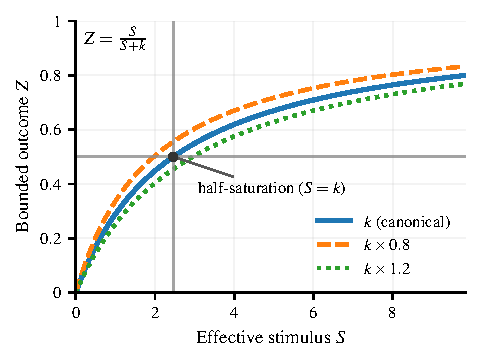
\includegraphics[width=\linewidth]{figure_1_saturation_curve.pdf}
  \end{minipage}%
  \hspace{0.03\linewidth}%
  \begin{minipage}[t]{0.58\linewidth}
    \vspace{0pt}
    \captionsetup{skip=0.2em}
    \caption{\textbf{Data scope:} schematic of the saturation transform that maps the effective stimulus $S=X^{\alpha}Y^{\beta}e^{\Phi}$ into a bounded outcome $Z\in(0,1)$ via $Z=\tfrac{S}{S+k}$. \textbf{Method context:} the curve highlights diminishing marginal gains as $S$ grows, and the dashed/dotted variants show how plausible perturbations of $k$ shift the transition horizontally while preserving the bounded range of $Z$. \textbf{Interpretation boundary:} this is a structural reading aid for the fitted model, not empirical validation, Tier A/B refit OOS evidence, or causal/policy evidence. The mid-curve inflection point and $Z=0.5$ ridge are geometric properties of the bounded-scale mapping, not independently validated behavioral thresholds.}
  \end{minipage}
\end{figure}
\noindent\justifying
\textit{Reading note.} Because contextual variables enter $\Phi$ on a standardized scale, coefficient magnitudes are
comparable on the log-exposure scale, but their translation into changes in $Z$ is not constant: the bounded map
implies that identical shifts in $\Phi$ have different consequences depending on baseline regime. The forest plot is
therefore treated as a parameter-diagnostic complement to the scenario-based effect summaries reported later.
{% 3-panel horizontal forest plot (main | interactions | quadratics)
\setlength{\textfloatsep}{6pt}
\setlength{\floatsep}{6pt}
\setlength{\abovecaptionskip}{\baselineskip}
\setlength{\belowcaptionskip}{0pt}
\begin{figure}[t]
  \centering
  
  \begin{minipage}[t]{0.32\linewidth}
    \centering
    \IfFileExists{figures/figure_3a_coefficients_forest_main.next.pdf}{%
      \includegraphics[width=\linewidth]{figures/figure_3a_coefficients_forest_main.next.pdf}%
    }{%
      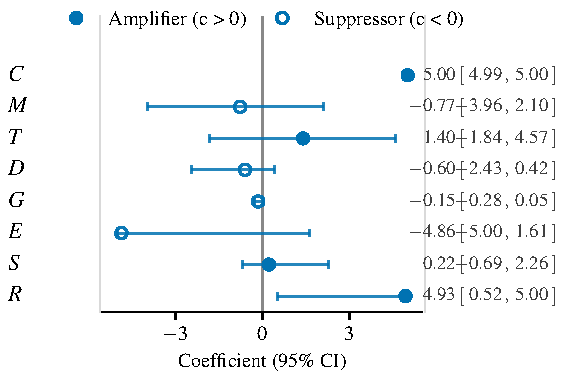
\includegraphics[width=\linewidth]{figure_3a_coefficients_forest_main.pdf}%
    }%
    \vspace{2pt}
    {\small\textbf{Main effects}}
  \end{minipage}%
  \hfill
  \begin{minipage}[t]{0.32\linewidth}
    \centering
    \IfFileExists{figures/figure_3b_coefficients_forest_interactions.next.pdf}{%
      \includegraphics[width=\linewidth]{figures/figure_3b_coefficients_forest_interactions.next.pdf}%
    }{%
      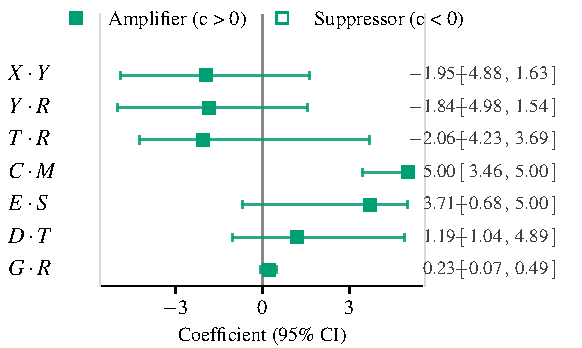
\includegraphics[width=\linewidth]{figure_3b_coefficients_forest_interactions.pdf}%
    }%
    \vspace{2pt}
    {\small\textbf{Interactions}}
  \end{minipage}%
  \hfill
  \begin{minipage}[t]{0.32\linewidth}
    \centering
    \IfFileExists{figures/figure_3c_coefficients_forest_quadratics.next.pdf}{%
      \includegraphics[width=\linewidth]{figures/figure_3c_coefficients_forest_quadratics.next.pdf}%
    }{%
      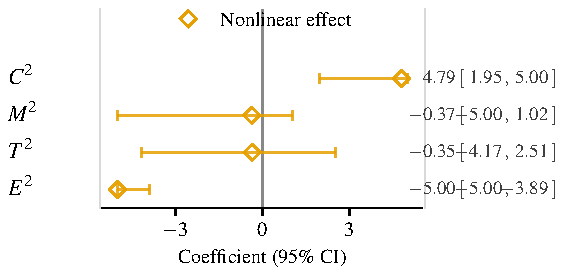
\includegraphics[width=\linewidth]{figure_3c_coefficients_forest_quadratics.pdf}%
    }%
    \vspace{2pt}
    {\small\textbf{Quadratics}}
  \end{minipage}
  
  \caption{\textbf{Data scope:} fitted coefficients for the contextual field $\Phi$ (Eq.~\eqref{eq:phi}) across main, interaction, and quadratic terms. \textbf{Method context:} this is a parameter-diagnostic view under the production-pinned coefficient contract encoded in \nolinkurl{src/data/feCoefficients.ts}; the left, center, and right panels report main effects, interactions, and quadratics respectively. \textbf{Interpretation boundary:} coefficient signs and intervals inform fitted-map geometry only; primary inferential evidence remains Tier A/B refit OOS results, while higher-order terms are support-constrained and non-causal.}
  \label{fig:coeff-forest-3panel}
\end{figure}
}
\noindent\justifying
\textit{Reading note.} The phase-style view formalizes why policy-facing reasoning should emphasize local leverage.
The derivative $\partial Z/\partial\Phi = Z(1-Z)$ peaks in the midrange and collapses near the bounds, so the same
intervention-sized perturbation can be consequential in a transition regime but negligible once the system is
already saturated.

\begin{figure}[t]
  \centering
  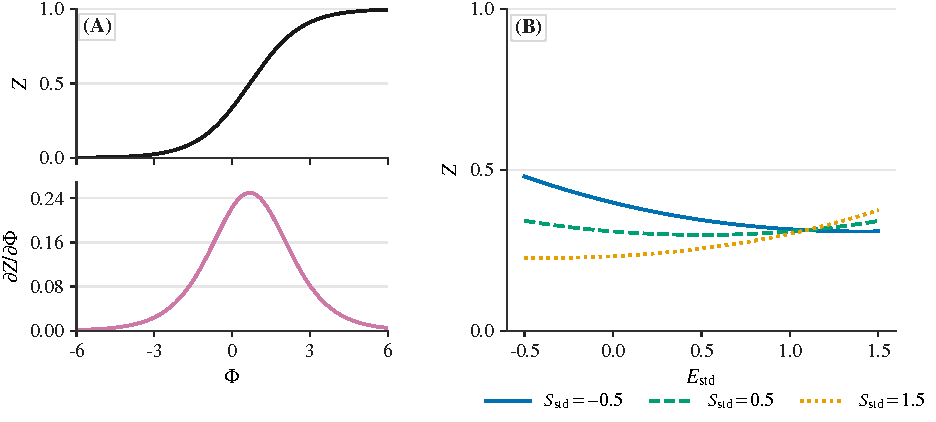
\includegraphics[width=0.96\linewidth]{figure_1_phase_policy.pdf}
  \caption{\textbf{Data scope:} model-implied bounded-response geometry and local sensitivity under the fitted preprocessing and parameter contract (Figure~S4). \emph{(A)} shows $Z(\Phi)=\tfrac{Be^{\Phi}}{Be^{\Phi}+k}$ and $\tfrac{\partial Z}{\partial \Phi}=Z(1-Z)$; \emph{(B)} shows policy-style slices of $Z$ versus $E_{\mathrm{std}}$ for selected $S_{\mathrm{std}}$ values under fixed stress settings. \textbf{Method context:} this is an in-sample geometry diagnostic generated under the same bounded-domain contract as the fitted model; primary inferential evidence remains Tier A/B refit OOS leave-one-country-out evaluation (the primary spatial validation pathway), with rolling-origin serving as a temporal scope diagnostic. \textbf{Interpretation boundary:} read at the country--year state level under thin support (49 complete-case observations) with uneven regime coverage; descriptive, non-causal, and not a policy-intervention estimate. The ridge at $Z=0.5$ reflects bounded-scale mapping geometry (maximum of $Z(1-Z)$), not an independently validated behavioral threshold.}
\end{figure}
\noindent\justifying
\textit{Reading note.} The reduced-coordinate geometry makes explicit that $Z$ depends on the sum $(\Phi+s)$, where
$s$ is the structural shift induced by $X$ and $Y$. Straight constant-$Z$ contours in the $(\Phi,s)$ plane and the
ridge at $Z=0.5$ provide a compact way to reason about regime changes as either (i) contextual shifts along $\Phi$
or (ii) structural shifts along $s$.

\begin{figure}[!htbp]
  \centering

  \newcommand{\FigureFiveCaption}{\textbf{Data scope:} reduced-coordinate geometry of the main function $Z=\sigma(\Phi+s)$ with $s:=\ln(B/k)$ (where $B=X^{\alpha}Y^{\beta}$) (Figure~S5). Values are computed in the interior band $(\varepsilon,1-\varepsilon)$ (here $\varepsilon=10^{-4}$), while the color scale is labeled by the conceptual endpoints $Z\in[0,1]$. \emph{(A)} Heatmap of $Z$ over $(\Phi,s)$ with constant-$Z$ contours and the ridge $Z=0.5$. \emph{(B)} Slices $Z(\Phi)$ at three shifts. \emph{(C)} Isometric surface of $Z(\Phi,s)$ with ridge and baseline slice overlaid. \textbf{Method context:} this is an in-sample geometry diagnostic; protocol interpretation is anchored to Tier A/B refit OOS leave-one-country-out evidence (the primary spatial validation pathway), with rolling-origin serving as a temporal scope diagnostic. \textbf{Interpretation boundary:} read as model-implied country--year geometry under thin support (49 complete-case observations) with uneven regime coverage; support-conditioned, non-causal, and not a transportability claim. The ridge at $Z=0.5$ is a geometric property of the bounded-scale mapping (maximum of $Z(1-Z)$), not an independently validated behavioral threshold.}

  \refstepcounter{figure}
  \addcontentsline{lof}{figure}{\protect\numberline{\thefigure}{\FigureFiveCaption}}
  \label{fig:main-function-views}

  \begin{tikzpicture}
    \node[inner sep=0] (img) {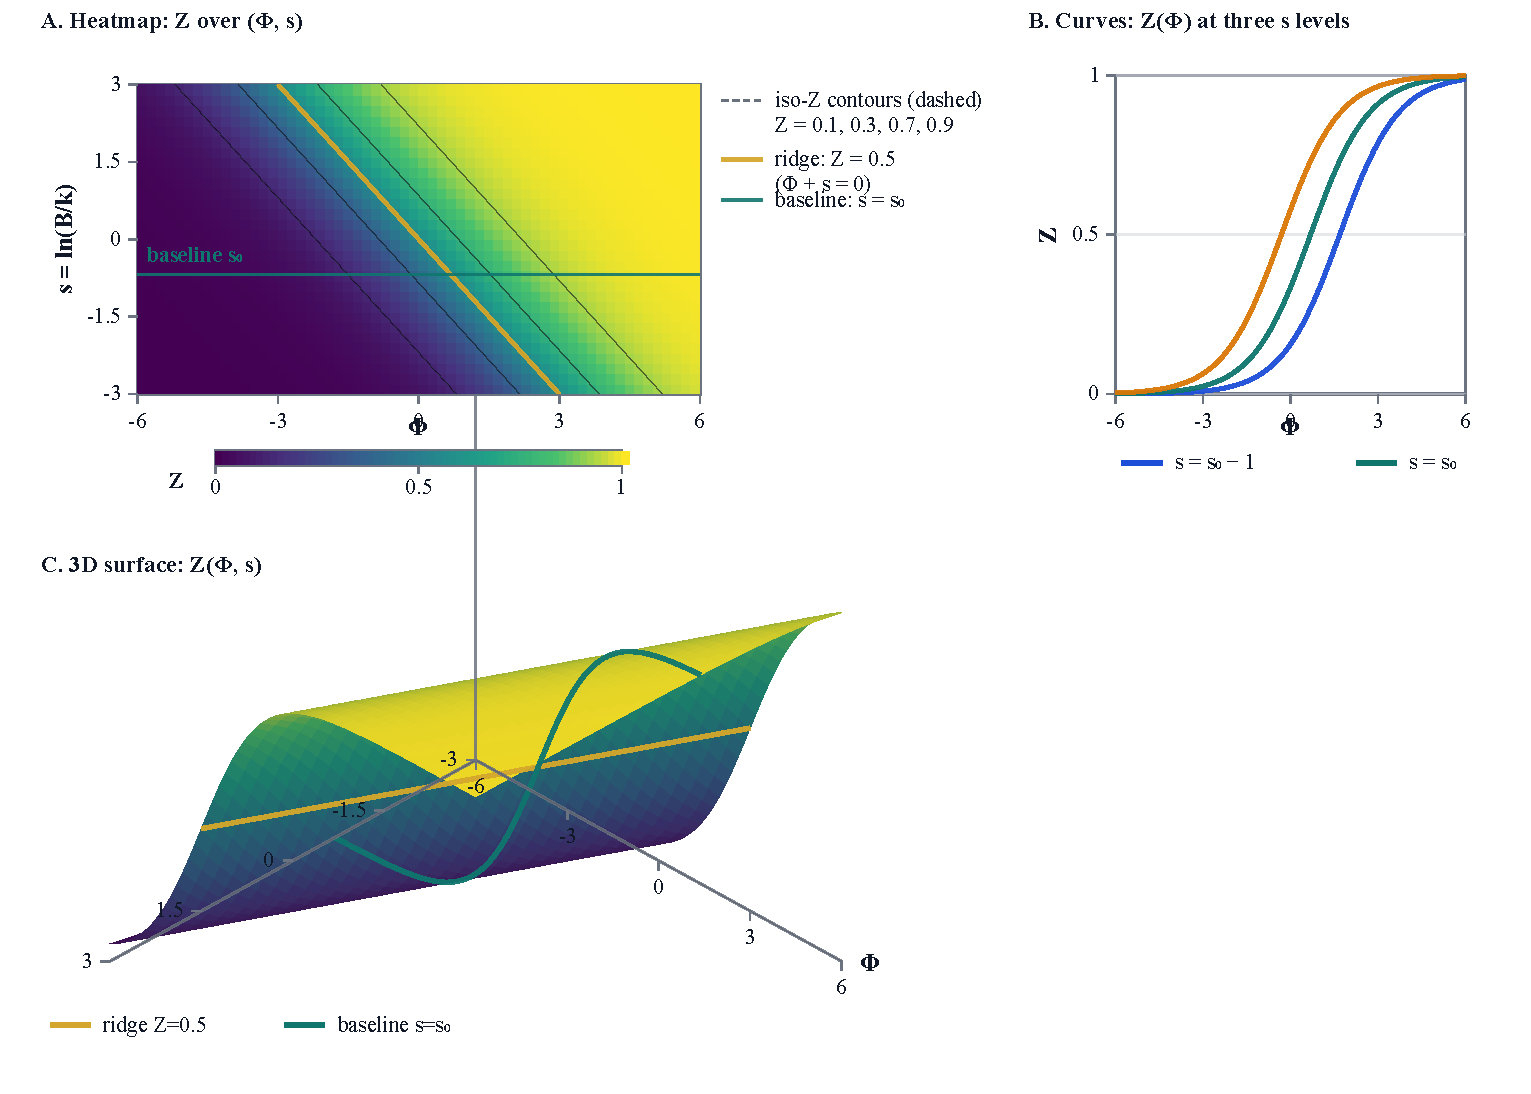
\includegraphics[width=\linewidth]{figure_2_main_function_geometry.pdf}};
    \begin{scope}[x={(img.south east)}, y={(img.north west)}]
      \node[
        anchor=north west,
        text width=0.39\linewidth,
        inner sep=0pt,
        outer sep=0pt
      ] at (0.63,0.47) {{\footnotesize\begin{minipage}{\linewidth}\setlength{\parindent}{0pt}\noindent\justifying\textbf{Figure~\thefigure.}~\itshape\FigureFiveCaption\end{minipage}}};
    \end{scope}
  \end{tikzpicture}
\end{figure}

\noindent\justifying
\textit{Context.} Evaluation is performed on the bounded-scale diagnostics used by the paper and tooling. The key
idea is to compare observed outcomes and predictions on a common interior band and to treat calibration and support
as first-class constraints. The robustness tables that follow are deterministic (no re-fit): they probe whether the
headline fit and regime geometry remain stable across temporal blocks and specification ablations. These robustness summaries belong to the fixed-model descriptive-diagnostic family and should be read together with, not in place of, refit OOS protocol evidence.
\begin{table}[t]
\centering
\TableStyle
\caption{\textbf{Data scope:} fixed-coefficient bounded-scale diagnostics across temporal blocks and structural ablations. \textbf{Method context:} all metrics use bounded observed outcomes and clamped predictions $\widehat{Z}\in\mathcal{I}_\varepsilon$; Panel A uses empirical year cutpoints 2006 and 2012, and Panel B compares main-only, main+interactions, and full (including quadratics) specifications without refitting coefficients. \textbf{Interpretation boundary:} this is a fixed-model descriptive diagnostic and is not part of the Tier A/B refit OOS inferential family or causal evidence.}
\label{tab:robustness_deterministic}
\begin{tabularx}{\linewidth}{@{}l l *{5}{>{\raggedleft\arraybackslash}X}@{}}
\toprule
Panel & Slice / Ablation & $n$ & $R^2$ & Corr & MAE & RMSE \\
\midrule
A & $\text{year}\le2005$ & 45 & \num{0.4115} & \num{0.6415} & \num{0.1231} & \num{0.1749} \\
A & $2006\le\text{year}\le2012$ & 65 & \num{0.6260} & \num{0.7921} & \num{0.1329} & \num{0.1827} \\
A & $\text{year}\ge2013$ & 57 & \num{0.6148} & \num{0.7841} & \num{0.1140} & \num{0.1447} \\
\addlinespace[2pt]
B & main ($\Phi$ linear only) & 167 & \num{0.4728} & \num{0.6877} & \num{0.1449} & \num{0.1904} \\
B & main$+$interactions & 167 & \num{0.5549} & \num{0.7450} & \num{0.1285} & \num{0.1749} \\
B & full (incl.\ quadratics) & 167 & \num{0.5642} & \num{0.7514} & \num{0.1260} & \num{0.1731} \\
\bottomrule
\end{tabularx}
\end{table}

\noindent\justifying
\textit{Reading note.} Training-time uncertainty summaries (cross-validation dispersion and bootstrap intervals)
provide an envelope for global performance and parameter stability during model construction, but they should not be
read as substitutes for the bounded-scale, support-aware diagnostics on the canonical panel. They are retained here as
provenance: they document that the reported mapping reflects a stable optimization basin rather than a single run.
\begin{table}[t]
\centering
\TableStyle
\caption{\textbf{Data scope:} training-time cross-validation dispersion and bootstrap uncertainty summaries for the fitted specification. \textbf{Method context:} CV values are reported as mean and standard deviation across folds with a 95\% half-width from fold dispersion, and bootstrap intervals provide 95\% CIs for global metrics. \textbf{Interpretation boundary:} this is a training-time provenance view, not a substitute for bounded-scale panel evaluation or Tier A/B refit OOS evidence, and it does not establish causal or policy-intervention claims.}
\label{tab:training_uq_summary}
\begin{tabularx}{0.92\linewidth}{@{}l *{5}{>{\raggedleft\arraybackslash}X}@{}}
\toprule
Metric & Train & CV mean & CV std & CV 95\% half-width & Bootstrap 95\% CI \\
\midrule
$R^2$ & \num{0.9481} & \num{0.9477} & \num{0.0101} & \num{0.0088} & [\num{0.9354},\ \num{0.9581}] \\
Corr & \num{0.9794} & \num{0.9795} & \num{0.0032} & \num{0.0028} & [\num{0.9752},\ \num{0.9830}] \\
MAE & \num{0.1341} & \num{0.1341} & \num{0.0142} & \num{0.0124} & [\num{0.1207},\ \num{0.1491}] \\
\bottomrule
\end{tabularx}
\end{table}

\noindent\justifying
\textit{Context.} The headline table reports global agreement on the bounded evaluation scale and is intended as a
compact summary of fit, not a guarantee of uniform validity across regimes. In a saturating system, strong rank
association can coexist with localized miscalibration; therefore, the supplemental diagnostic figures that follow in
this file (observed-vs-predicted, calibration-by-decile, and residual structure) are treated as essential evidence.
\begin{table}[!htbp]
\centering
\TableStyle
\captionsetup{justification=RaggedRight,singlelinecheck=false}
\caption{\textbf{Data scope:} bounded-scale in-sample evaluation on the canonical panel. Observed $Z$ is mapped into $\mathcal{I}_\varepsilon$ using the bounded-scale mapping with $(z_{\min},z_{\max})=(\num{-1.8892873085},\,\num{1.8541262393})$ and $\varepsilon=10^{-4}$; predictions are clamped to the same band, and bias is the mean residual $(Z-\widehat{Z})$. \textbf{Method context:} the evidence tier for this table is descriptive context only; primary inferential claims rest on Tier A/B out-of-sample refit validation detailed in the Fold-Level Generalization Evidence section. \textbf{Interpretation boundary:} the panel is 167 complete-case country-years across 76 countries with no scenario replication, so the row count is the support count, and the table does not by itself support causal or policy-intervention claims.}
\label{tab:panel_fit_headline}
\begin{tabularx}{0.86\linewidth}{@{}l >{\raggedleft\arraybackslash}X@{}}

\csname toprule\endcsname
Quantity & Value \\
\midrule
Countries ($N$) & 48 \\
Rows used ($n$) & 87 \\
Year range & 1990--2023 \\
$R^2$ & \num{0.2516} \\
$\mathrm{Corr}(Z,\widehat{Z})$ & \num{0.6311} \\
MAE & \num{0.1498} \\
RMSE & \num{0.1893} \\
Bias $(Z-\widehat{Z})$ & \num{0.0243} \\
\bottomrule
\end{tabularx}
\end{table}

\noindent\justifying
\textit{Reading note.} To connect the fitted mapping to scenario inspection in the interactive system, this supplement reports
country-preset summaries and regime-based finite differences. These artifacts make it explicit that the same
coefficient map can imply different bounded-scale changes depending on baseline regime, which is why scenario-based
effect sizes ($\Delta Z$ under controlled perturbations) are emphasized over purely local derivative intuition.
\noindent\justifying
In particular, preset summaries should be read as \emph{state anchors}: they represent reproducible, named operating points where both the decomposition of $\Phi$ and the bounded-scale sensitivity are fixed.
This makes it possible to distinguish disagreements attributable to (i) shifts in contextual composition versus (ii) shifts in structural baseline $(X,Y)$, under the same coefficient contract.
In review terms, this table is best read as a compact within-paper consistency check: the preset outcomes can be recomputed from the pinned coefficients and preprocessing bounds, and therefore provide a quick sanity test that the evidence bundle is internally coherent.
Because the presets are defined at the panel-average level, they also function as a ``unit test'' for the full preprocessing pipeline: if a preset outcome disagrees with its recomputation, the discrepancy typically indicates a mismatch in standardization bounds, clamping, or coefficient key mapping rather than a substantive modeling issue.
Accordingly, readers are encouraged to interpret the preset rows as reference points for the subsequent regime-difference tables and curves.

\begin{table}[!htbp]
\centering
\TableStyle
\caption{\textbf{Data scope:} preset-country panel alignment between year-averaged observed and predicted bounded outcomes. For each country preset, measured values are the canonical panel outcome normalized into $[\varepsilon,1-\varepsilon]$ (with $\varepsilon=10^{-4}$) and averaged across unique years; predicted values use canonical preprocessing. \textbf{Method context:} MAE is computed on year-averaged pairs and Success (\%) = $100(1-\mathrm{MAE})$ on the bounded scale; Estonia, Russia, and Slovak Republic are flagged because their presets occupy sparse or volatile support regimes. \textbf{Interpretation boundary:} this is a fixed-contract descriptive alignment table, not Tier A/B refit OOS evidence; flagged-country readings are exploratory and the table does not support causal or policy-intervention claims.}
\label{tab:preset-country-z}
\begin{tabularx}{\linewidth}{@{}l l r *{5}{>{\raggedleft\arraybackslash}X} c c c@{}}
\toprule
Country & ISO3 & Years & $\overline{Z}$ & $\overline{\widehat{Z}}$ & MAE & Success (\%) & Bias $(\overline{Z}-\overline{\widehat{Z}})$ & Good & Accept. & Poor \\
\midrule
Australia & AUS & 1 & 0.174 & 0.223 & 0.050 & 95.0 & -0.050 & \textcolor{green!50!black}{$\boldsymbol{\checkmark}$} &  &  \\
Brazil & BRA & 1 & 0.836 & 0.970 & 0.134 & 86.6 & -0.134 &  & \textcolor{green!35!black}{\textbf{+}} &  \\
Bulgaria & BGR & 1 & 0.414 & 0.582 & 0.168 & 83.2 & -0.168 &  & \textcolor{green!35!black}{\textbf{+}} &  \\
Canada & CAN & 3 & 0.461 & 0.528 & 0.067 & 93.3 & -0.067 & \textcolor{green!50!black}{$\boldsymbol{\checkmark}$} &  &  \\
Chile & CHL & 1 & 0.679 & 0.811 & 0.132 & 86.8 & -0.132 &  & \textcolor{green!35!black}{\textbf{+}} &  \\
Czechia & CZE & 1 & 0.000 & 0.133 & 0.133 & 86.7 & -0.133 &  & \textcolor{green!35!black}{\textbf{+}} &  \\
Estonia & EST & 1 & 0.103 & 0.396 & 0.292 & 70.8 & -0.292 &  &  & \textcolor{red!70!black}{$\boldsymbol{\times}$} \\
Finland & FIN & 1 & 0.387 & 0.334 & 0.054 & 94.6 & 0.054 & \textcolor{green!50!black}{$\boldsymbol{\checkmark}$} &  &  \\
Germany & DEU & 2 & 0.205 & 0.299 & 0.094 & 90.6 & -0.094 & \textcolor{green!50!black}{$\boldsymbol{\checkmark}$} &  &  \\
Greece & GRC & 1 & 0.849 & 0.939 & 0.089 & 91.1 & -0.089 & \textcolor{green!50!black}{$\boldsymbol{\checkmark}$} &  &  \\
Korea & KOR & 2 & 0.382 & 0.488 & 0.106 & 89.4 & -0.106 &  & \textcolor{green!35!black}{\textbf{+}} &  \\
Mexico & MEX & 2 & 0.835 & 0.925 & 0.090 & 91.0 & -0.090 & \textcolor{green!50!black}{$\boldsymbol{\checkmark}$} &  &  \\
Netherlands & NLD & 2 & 0.114 & 0.113 & 0.082 & 91.8 & 0.001 & \textcolor{green!50!black}{$\boldsymbol{\checkmark}$} &  &  \\
Poland & POL & 2 & 0.826 & 0.922 & 0.096 & 90.4 & -0.096 & \textcolor{green!50!black}{$\boldsymbol{\checkmark}$} &  &  \\
Romania & ROU & 2 & 0.850 & 0.916 & 0.066 & 93.4 & -0.066 & \textcolor{green!50!black}{$\boldsymbol{\checkmark}$} &  &  \\
Russia & RUS & 2 & 0.373 & 0.624 & 0.250 & 75.0 & -0.250 &  &  & \textcolor{red!70!black}{$\boldsymbol{\times}$} \\
Slovak Republic & SVK & 1 & 0.423 & 0.146 & 0.277 & 72.3 & 0.277 &  &  & \textcolor{red!70!black}{$\boldsymbol{\times}$} \\
Slovenia & SVN & 1 & 0.299 & 0.200 & 0.099 & 90.1 & 0.099 & \textcolor{green!50!black}{$\boldsymbol{\checkmark}$} &  &  \\
Spain & ESP & 2 & 0.202 & 0.264 & 0.062 & 93.8 & -0.062 & \textcolor{green!50!black}{$\boldsymbol{\checkmark}$} &  &  \\
Switzerland & CHE & 1 & 0.346 & 0.460 & 0.113 & 88.7 & -0.113 &  & \textcolor{green!35!black}{\textbf{+}} &  \\
T{\"u}rkiye & TUR & 2 & 0.979 & 0.992 & 0.021 & 97.9 & -0.013 & \textcolor{green!50!black}{$\boldsymbol{\checkmark}$} &  &  \\
United Kingdom & GBR & 1 & 0.312 & 0.406 & 0.094 & 90.6 & -0.094 & \textcolor{green!50!black}{$\boldsymbol{\checkmark}$} &  &  \\
United States & USA & 1 & 0.517 & 0.447 & 0.070 & 93.0 & 0.070 & \textcolor{green!50!black}{$\boldsymbol{\checkmark}$} &  &  \\
\bottomrule
\end{tabularx}
\vspace{2pt}
{\footnotesize \textit{Note.} Classification thresholds: good if MAE $\le 0.10$; acceptable if 0.10 $<$ MAE $\le 0.20$; poor if MAE $> 0.20$.}
\end{table}

\noindent\justifying
\textit{Reading note.} The regime-based finite differences below are designed to be comparable across modifiers by holding a common contextual backdrop and applying a standardized +1 SD perturbation.
Because the bounded map compresses extremes, a large $\Delta\Phi$ does not necessarily imply a large $\Delta Z$ if the baseline is already near saturation; conversely, modest contextual shifts can produce large bounded-scale changes near the transition ridge.
As a result, the most interpretable comparisons are those that keep the baseline in the interior band and treat shifts toward the bounds as a change in available leverage rather than a change in mechanism direction.

\begin{table}[!htbp]
\centering
\TableStyle
\caption{\textbf{Data scope:} model-implied finite-difference $\Delta Z$ values under a +1 SD shock in each standardized modifier, evaluated at low/mid/high structural baselines. Baselines use $(X,Y)\in\{(0.2,0.2),(0.5,0.5),(0.8,0.8)\}$ in the structural interior band under a fixed contextual state $(M_{\mathrm{std}}=0.8,T_{\mathrm{std}}=1.2,D_{\mathrm{std}}=0.6)$, with baseline predictions $Z\approx 0.004$, $0.033$, and $0.053$. \textbf{Method context:} coefficients follow the production-pinned contract (\nolinkurl{src/data/feCoefficients.ts}) and bracketed ranges are precomputed diagnostic uncertainty bands for the fixed scenario contract. \textbf{Interpretation boundary:} these are regime-dependent scenario diagnostics, not causal or policy-intervention estimates; Tier A/B inferential anchors remain refit OOS evidence, and interval width in saturated regions mainly reflects bounded-map flatness rather than transportable precision. \textbf{Note:} $C_{\mathrm{std}}$ is derived from WVS cultural-practice items sharing source survey with the outcome~$Z$; the large marginal effect partially reflects this shared-source construction and should be interpreted with that overlap in mind.}
\label{tab:marginal-effects-regimes}
{\setlength{\tabcolsep}{2pt}%
\begin{tabularx}{\linewidth}{@{} l >{\raggedleft\arraybackslash}X >{\raggedleft\arraybackslash}X >{\raggedleft\arraybackslash}X @{} }
\toprule
Modifier (+1 SD) & $\Delta Z$ (low baseline) & $\Delta Z$ (mid baseline) & $\Delta Z$ (high baseline) \\
\midrule
\ensuremath{C_{\mathrm{std}}} (cultural intensity) & 0.9953 [0.1016, 0.9980] & 0.9670 [0.0259, 0.9979] & 0.9473 [0.0138, 0.9978] \\
\ensuremath{M_{\mathrm{std}}} (media environment) & -0.0037 [-0.4142, 0.5546] & -0.0269 [-0.6299, 0.5476] & -0.0427 [-0.7050, 0.5306] \\
\ensuremath{T_{\mathrm{std}}} (trauma/shock) & 0.0066 [-0.0311, 0.9507] & 0.0451 [-0.0997, 0.9057] & 0.0687 [-0.1586, 0.8907] \\
\ensuremath{D_{\mathrm{std}}} (social atomization) & 0.0057 [-0.0793, 0.6853] & 0.0393 [-0.2036, 0.6849] & 0.0601 [-0.2034, 0.6787] \\
\ensuremath{G_{\mathrm{std}}} (redistribution capacity) & -0.0006 [-0.0527, 0.0025] & -0.0045 [-0.0598, 0.0046] & -0.0070 [-0.0624, 0.0056] \\
\ensuremath{E_{\mathrm{std}}} (education capacity) & -0.0044 [-0.8666, 0.0000] & -0.0328 [-0.9636, 0.0000] & -0.0525 [-0.9691, 0.0000] \\
\ensuremath{S_{\mathrm{std}}} (social support) & 0.0011 [-0.0927, 0.2231] & 0.0078 [-0.1259, 0.2611] & 0.0122 [-0.1243, 0.2589] \\
\ensuremath{R_{\mathrm{std}}} (welfare capacity) & 0.0305 [-0.0992, 0.8398] & 0.1036 [-0.3277, 0.8192] & 0.0767 [-0.4333, 0.7992] \\
\bottomrule
\end{tabularx}
}
\end{table}
\noindent\justifying
\textit{Reading note.} The marginal-effect curves visualize effect heterogeneity across the interior band and
highlight where the bounded map is most sensitive. Robust variants later in this file add sensitivity envelopes,
helping distinguish stability due to true robustness from apparent stability caused by saturation.
In particular, the curves should be read as regime-conditional summaries: where the slope is steep, small contextual changes can produce meaningful bounded-scale differences; where the curve flattens, the same contextual perturbation may be computationally detectable but substantively negligible.

\begin{figure}[t]
  \centering
  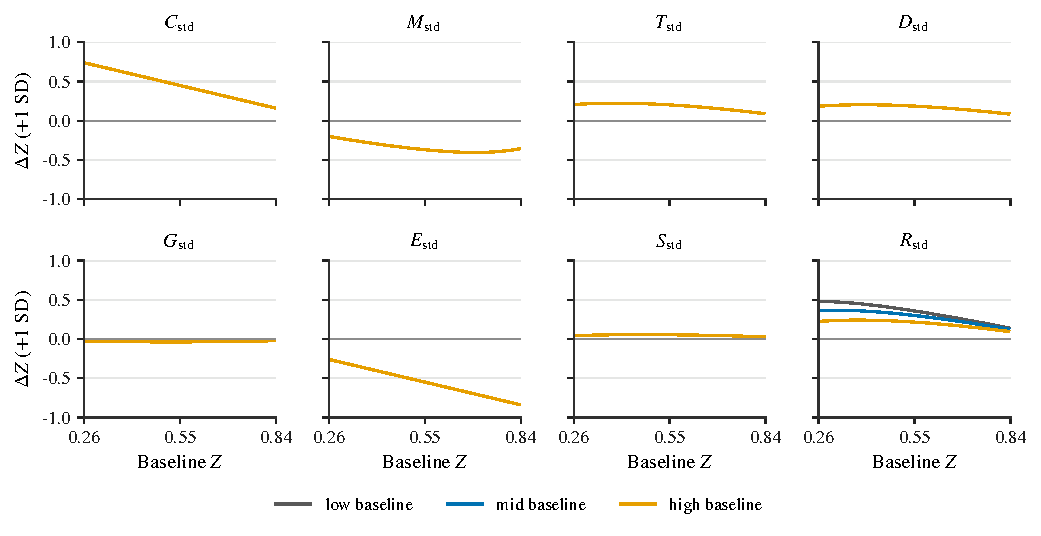
\includegraphics[width=\linewidth]{figure_12_marginal_effect_curves.pdf}
  \caption{\textbf{Data scope:} scenario-based marginal-effect curves showing $\Delta Z$ under +1 SD shocks as a function of baseline prediction $Z$. Curves are shown for three structural baselines in the interior band $(X,Y)\in\{(0.2,0.2),(0.5,0.5),(0.8,0.8)\}$ under the same fixed contextual state used in Table~\ref{tab:marginal-effects-regimes}; the baseline-$Z$ axis is restricted to an empirically supported interior range from sensitivity-weighted quantiles of the canonical panel. \textbf{Method context:} coefficients follow the production-pinned contract (\nolinkurl{src/data/feCoefficients.ts}) and the plot exposes regime dependence under the same fixed scenario contract as the table. \textbf{Interpretation boundary:} these are model-implied regime-conditional associations, not causal response functions or Tier A/B refit OOS validation results. The regime sensitivity pattern ($\Delta Z$ peaking near $Z=0.5$) reflects bounded-scale mapping geometry, not an independently validated behavioral threshold.}
  \label{fig:marginal-effect-curves}
\end{figure}

\noindent\justifying
\textit{Context.} The amplifier/suppressor view translates the fitted contextual field into a local, auditable
mechanism narrative. The intent is interpretability under regime dependence: a channel’s directional role is defined
by its local contribution to $\Phi$ at a scenario state, while its observable impact on $Z$ is additionally scaled by
state-dependent sensitivity. This supports disciplined interpretation without overstating causal identification.
{% Documentation Section 3 (Amplifiers) — two-panel schematic (re-rendered for paper)
\setlength{\textfloatsep}{2pt}
\setlength{\floatsep}{2pt}
\setlength{\abovecaptionskip}{2pt}
\setlength{\belowcaptionskip}{0pt}
\begin{figure}[tbp]
  \centering

  \begin{minipage}[t]{0.49\linewidth}
    \centering
    \IfFileExists{figures/fig_doc_section3_phase_transition.next.pdf}{%
      \includegraphics[width=0.98\linewidth]{figures/fig_doc_section3_phase_transition.next.pdf}%
    }{%
      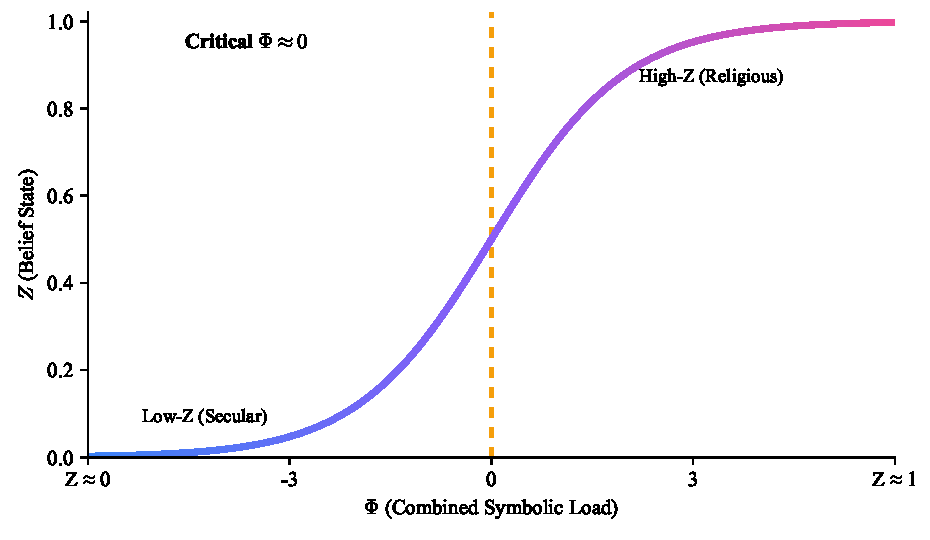
\includegraphics[width=0.98\linewidth]{fig_doc_section3_phase_transition.pdf}%
    }%
    \vspace{0pt}
    {\small\textbf{(A)} Phase-transition schematic}
  \end{minipage}%
  \hfill
  \begin{minipage}[t]{0.49\linewidth}
    \centering
    \IfFileExists{figures/fig_doc_section3_energy_field.next.pdf}{%
      \includegraphics[width=0.98\linewidth]{figures/fig_doc_section3_energy_field.next.pdf}%
    }{%
      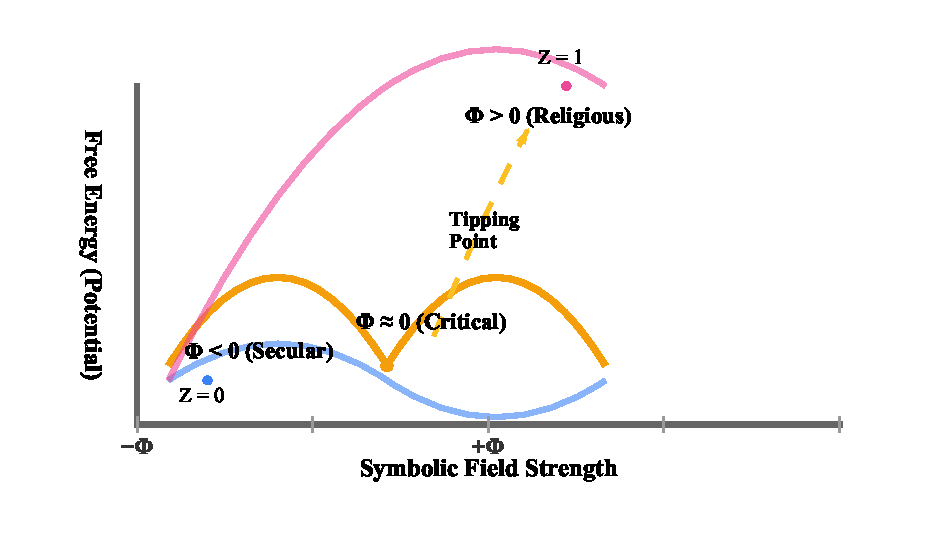
\includegraphics[width=0.98\linewidth]{fig_doc_section3_energy_field.pdf}%
    }%
    \vspace{0pt}
    {\small\textbf{(B)} Energy-field intuition}
  \end{minipage}

  \caption{\textbf{Data scope:} documentation schematics used in the Section~3 exposition. \textbf{Method context:} Panel \textbf{(A)} shows the bounded response $Z(\Phi)$ around the transition region, and Panel \textbf{(B)} shows the potential-landscape analogy and tipping direction used to explain the mechanism. \textbf{Interpretation boundary:} these are explanatory schematics only; they are not empirical evidence, evidence-tier support, or causal identification. The transition region around $Z \approx 0.5$ reflects bounded-scale mapping geometry.}
\end{figure}
}

\endgroup

\Section{Additional supplementary figures (pipeline, evaluation, and diagnostics)}
\noindent\justifying
This section contains supplementary-only figures used to document the pipeline, evaluation diagnostics, robustness
variants, correlation structure, and the visual analytics tooling.

{%
\setlength{\intextsep}{6pt}% space above/below in-text floats (incl. [H])
\setlength{\textfloatsep}{6pt}% space between floats and text (top/bottom)
\setlength{\floatsep}{6pt}% space between floats
\setlength{\abovecaptionskip}{\baselineskip}% space between graphic and caption
\setlength{\belowcaptionskip}{0pt}% space after caption
\begin{figure}[!htbp]
\begingroup
\footnotesize
\setlength{\parskip}{0pt}% avoid unintended gaps between boxed rows
\setlength{\parindent}{0pt}% avoid any left indent (keeps boxes perfectly aligned)
\setlength{\fboxsep}{2.5pt}
\setlength{\fboxrule}{0.4pt}
\newlength{\PipelineSeamOverlap}
\setlength{\PipelineSeamOverlap}{0.9pt}
\setlength{\extrarowheight}{0pt}% eliminate extra space in rows
\renewcommand{\arraystretch}{1.0}% avoid surprising side-effects (Context sets its own)
\newcommand{\PipelineCell}[3][white]{%
\fcolorbox{black!65}{#1}{%
\begin{minipage}[c]{\dimexpr\linewidth-2\fboxsep-2\fboxrule\relax}
\centering
{\bfseries #2}\par
\vspace{0.15em}
{#3}
\end{minipage}%
}%
}%
\newlength{\PipelineStepBoxHeight}
\setlength{\PipelineStepBoxHeight}{1.95cm}
\newcommand{\PipelineStepCell}[3][white]{%
\fcolorbox{black!65}{#1}{%
\begin{minipage}[c][\PipelineStepBoxHeight][c]{\dimexpr\linewidth-2\fboxsep-2\fboxrule\relax}
\centering
{\bfseries #2}\par
\vspace{0.15em}
{#3}
\end{minipage}%
}%
}%
\noindent\begin{minipage}[t]{0.67\linewidth}
\vspace{0pt}% anchor top alignment
\raggedright
\newlength{\PipelineHalfColWidth}
\setlength{\PipelineHalfColWidth}{\dimexpr0.5\linewidth+0.5\PipelineSeamOverlap\relax}
\newcommand{\PipelineRow}[2]{%
\hbox{%
\begin{minipage}[t]{\PipelineHalfColWidth}#1\end{minipage}%
\hspace{-\PipelineSeamOverlap}% overlap middle borders: no white seam, single rule
\begin{minipage}[t]{\PipelineHalfColWidth}#2\end{minipage}%
}%
}%
\vbox{\offinterlineskip
\hbox{\begin{minipage}[t]{\linewidth}%
\PipelineCell[blue!6]{1. Context field ($\PhiField$)}{%
\(\PhiField = \phiZero + \Phi_{\mathrm{main}} + \Phi_{\mathrm{int}} + \Phi_{\mathrm{quad}}\)\par
\vspace{0.12em}
{\renewcommand{\arraystretch}{1.05}%
\begin{tabularx}{\linewidth}{@{}>{\centering\arraybackslash}X>{\centering\arraybackslash}X@{}}
Main: \(C_{\mathrm{std}}, M_{\mathrm{std}}, T_{\mathrm{std}}, D_{\mathrm{std}}, G_{\mathrm{std}}, E_{\mathrm{std}}, S_{\mathrm{std}}, R_{\mathrm{std}}\) & Amp (+): \(C,\,T,\,S,\,R\)\\
Interactions: \(XY,\allowbreak\; YR_{\mathrm{std}},\allowbreak\; T_{\mathrm{std}}R_{\mathrm{std}},\allowbreak\; C_{\mathrm{std}}M_{\mathrm{std}},\allowbreak\; E_{\mathrm{std}}S_{\mathrm{std}},\allowbreak\; D_{\mathrm{std}}T_{\mathrm{std}},\allowbreak\; G_{\mathrm{std}}R_{\mathrm{std}}\) & Sup ($-$): \(M,\,D,\,G,\,E\)\\
Quadratics: \(C_{\mathrm{std}}^{2},\; M_{\mathrm{std}}^{2},\; T_{\mathrm{std}}^{2},\; E_{\mathrm{std}}^{2}\) & \\
\end{tabularx}
}
}%
\end{minipage}}%
\kern-\PipelineSeamOverlap
\PipelineRow{%
\PipelineStepCell[gray!8]{2. Inputs}{%
Raw drivers: \(\X_{\mathrm{raw}},\,\Y_{\mathrm{raw}}\)\\
Context (std): \(C_{\mathrm{std}}, M_{\mathrm{std}}, T_{\mathrm{std}}, D_{\mathrm{std}}, G_{\mathrm{std}}, E_{\mathrm{std}}, S_{\mathrm{std}}, R_{\mathrm{std}}\)
}%
}{%
\PipelineStepCell[orange!10]{4. Stimulus}{%
\(S = \X^{\alphaS}\,\Y^{\betaS}\,e^{\PhiField}\)\\
\(\log S = \alphaS\log \X + \betaS\log \Y + \PhiField\)
}%
}%
\kern-\PipelineSeamOverlap
\PipelineRow{%
\PipelineStepCell[green!7]{3. Safe band}{%
Band map (deterministic)\\
\(\X,\Y \in (\varepsilon, 1-\varepsilon)\)\\
\(\X = \mathrm{clip}(\mathrm{minmax}(\X_{\mathrm{raw}}),\,\varepsilon,\,1-\varepsilon)\); similarly \(\Y\)
}%
}{%
\PipelineStepCell[purple!8]{5. Saturation}{%
\(\Z = \dfrac{S}{S+\kappaS}\)\\
\(S = \kappaS\,\dfrac{\Z}{1-\Z}\); \(\kappaS\): half-saturation (\(\Z=0.5\))
}%
}%
}% end vbox
\end{minipage}%
\hfill
\begin{minipage}[t]{0.30\linewidth}
\vspace{0pt}% anchor top alignment
\captionsetup{justification=justified,singlelinecheck=false}
\caption{\textbf{Data scope:} end-to-end computational pipeline for the implemented belief-emergence mechanism. \textbf{Method context:} the figure traces construction of $\Phi$, deterministic preprocessing into the interior safe band, stimulus formation $S=X^{\alpha_{S}}Y^{\beta_{S}}e^{\Phi}$, and half-saturation mapping $Z=S/(S+\kappa_{S})$ under the production computational contract. \textbf{Interpretation boundary:} this is a reproducibility schematic that documents how quantities are computed; it does not itself validate fit, assign an evidence tier, or support causal interpretation.}
\label{fig:model-pipeline}
\end{minipage}
\endgroup
\end{figure}
}
\Section{Evaluation diagnostics (bounded-scale fit and residual structure)}
\noindent\justifying
The following evaluation plots reproduce the manuscript’s bounded-scale diagnostics. They are retained
verbatim (same width settings) to ensure that visual comparability is not confounded by re-scaling. These diagnostic figures are critical for assessing whether the bounded model achieves acceptable predictive accuracy and whether residuals exhibit problematic structure.
\noindent\justifying
Calibration on deciles of $\widehat{Z}$ provides a coarse but robust summary of conditional central tendency and dispersion;
departures from the 45$^\circ$ line indicate bias localized to predicted levels. Residual histograms characterize
marginal fit quality, while residual-versus-predicted displays reveal potential heteroskedasticity or state-dependent
misspecification. Because the evaluation is performed on the bounded support $\mathcal{I}_\varepsilon$, extreme values are
clamped for numerical stability, avoiding spurious leverage from saturation regions. The first figure in this section presents the observed versus predicted scatterplot and calibration-by-decile analysis, while the second shows marginal residual distribution and residual-versus-predicted diagnostics to detect any systematic patterns in the errors.
\noindent\justifying
Checking for model misspecification across prediction levels is essential because non-linearity and bounded response can mask systematic bias. Examination of decile-wise calibration can identify whether certain regimes (e.g., low, medium, or high predicted levels) suffer from consistent under- or over-prediction. The width of the IQR bands also reveals whether prediction uncertainty is constant or varies with predicted level. Heteroskedasticity in the residuals would manifest as a funnel pattern in the residual-versus-predicted plot, suggesting that the model's predictive variance is not homogeneous across the support.
\begin{figure}[!htbp]
    \centering
    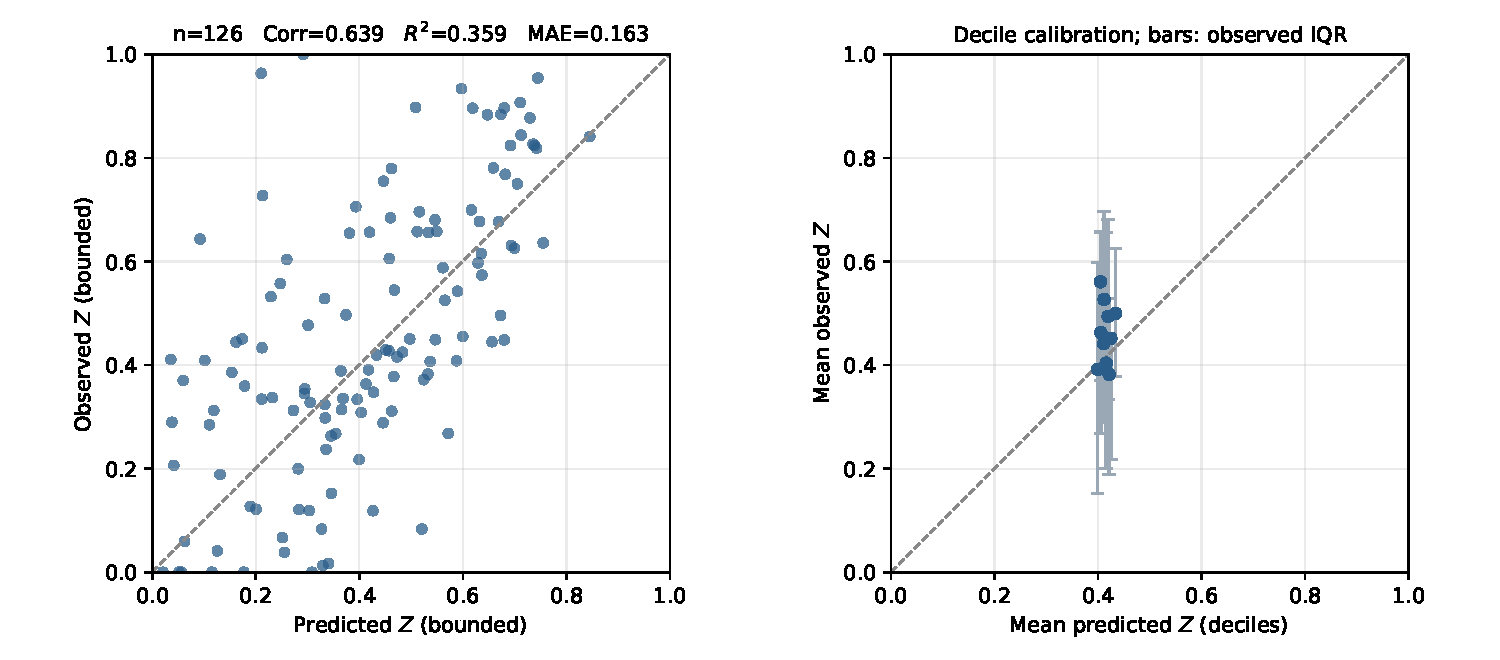
\includegraphics[width=\linewidth]{fig_eval_pair.pdf}
    \caption{\textbf{Data scope:} bounded-scale in-sample fit and decile-calibration diagnostics on the canonical panel. Observed outcomes $Z$ and predictions $\widehat{Z}$ are evaluated on the same bounded scale $\mathcal{I}_\varepsilon=[\varepsilon,1-\varepsilon]$ with $\varepsilon=10^{-4}$, and predictions are clamped for numerical stability. \textbf{Method context:} the left panel shows observed-versus-predicted values with hexagonal support density, while the right panel reports decile-wise mean $Z$ and within-decile $\mathrm{IQR}(Z)$ conditional on predicted level. \textbf{Interpretation boundary:} this figure provides descriptive fit context only; primary inferential weight remains Tier A/B refit OOS evidence, and the figure does not by itself support causal or policy claims.}
\end{figure}
\noindent\justifying
\textit{Reading note.} These plots should be read jointly: strong global agreement can coexist with localized calibration departures.
If the calibration curve deviates systematically in the low or high deciles, that pattern should be interpreted as regime-dependent bias rather than noise, and it should be cross-checked against the residual-versus-$\widehat{Z}$ trend in the next figure.
\begin{figure}[!htbp]
    \centering
    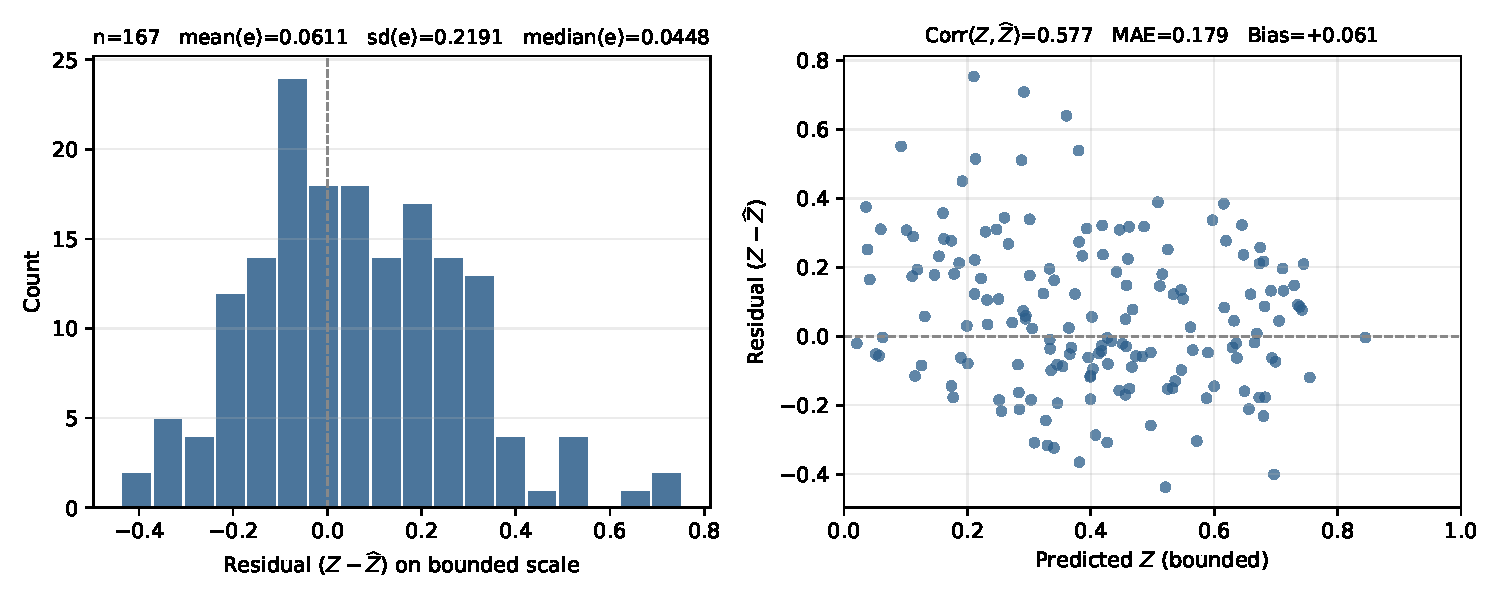
\includegraphics[width=\linewidth]{fig_eval_resid_pair.pdf}
    \caption{\textbf{Data scope:} bounded-scale residual diagnostics on the canonical panel. Residuals are computed as $e_i=Z_i-\widehat{Z}_i$ using bounded observed outcomes and clamped predictions in $\mathcal{I}_\varepsilon$. \textbf{Method context:} the left panel summarizes the marginal error distribution with a histogram and zero reference line, and the right panel screens for state-dependent bias or heteroskedasticity using residuals versus predicted $\widehat{Z}$ with a decile-binned mean overlay. \textbf{Interpretation boundary:} this is a descriptive misspecification screen only; it is not primary inferential evidence and does not support causal interpretation.}
\end{figure}
\Section{Regime-dependent effects and correlation diagnostics}
\noindent\justifying
This block aggregates the manuscript’s regime-aware marginal-effect visualizations and descriptive
correlation diagnostics. Keeping them adjacent makes it easier to interpret effect heterogeneity in light
of covariate dependence and potential collinearity structure.
\noindent\justifying
\textit{Reading note.} In tables and plots that report standardized variables (e.g., $C_{\mathrm{std}}$, $M_{\mathrm{std}}$), the scientific interpretation is inherently relative: a +1 SD perturbation represents a move that is large enough to be comparable across contexts, but it is not necessarily large in absolute units.
Accordingly, the regime panels are treated as a comparative map of \emph{where} and \emph{when} the model expresses sensitivity, not as an assertion that every standardized shift corresponds to an equally feasible real-world intervention.
This framing is particularly important near the bounded endpoints, where the same standardized shift can produce a small $\Delta Z$ purely because the map is locally flat.
\noindent\justifying
Marginal effects are computed as finite differences $\Delta Z$ under +1 SD perturbations to standardized modifiers,
holding a fixed contextual backdrop while varying structural baselines in the interior band. Because $Z$ is bounded
and monotone in $\Phi$ only after transformation, the \emph{size and sign} of $\Delta Z$ naturally depend on the baseline
level and local curvature of $\Phi$. Robust variants summarize sensitivity bands, clarifying which regimes are most
stable to perturbations. Correlation heatmaps provide a descriptive view of covariate dependence; they are included as
context for interpreting effect sizes without conflating inference with collinearity. Figure~11 and its variants (Figures~12 main and robust) show how marginal effects vary across different regimes and parameter ranges, while Figures~A2 and A3 document the overall and within-panel correlation structures to support interpretation of the empirical relationships.
\noindent\justifying
The importance of regime-dependent effects lies in recognizing that the bounded response is inherently non-linear. A modifier that is a strong amplifier in one region of the parameter space (e.g., where $\Phi$ is near zero and sensitivity is high) may have negligible or even inverted effects in saturation regions (where $\Phi$ is far from zero and the bounded transform is nearly flat). Robust marginal effects encompass ranges rather than point estimates, providing guidance on which regimes are most stable and informative. This multi-scale perspective prevents over-interpretation of effects in unstable regions and focuses attention on the regime where the model's predictive capability and parameter interpretability are strongest.
\noindent\justifying
\textit{Reading note.} Robust marginal-effect envelopes should be interpreted as an uncertainty-aware \emph{stability screen}: narrow bands indicate that the qualitative regime narrative is insensitive to perturbations, while wide bands flag regions where conclusions depend strongly on specification or sampling variation.
In practice, the most policy-relevant regimes are those with both (i) high local sensitivity (interior band) and (ii) stable envelopes.
When bands widen near saturation, this should generally be interpreted as low information rather than high disagreement: once $Z$ is effectively flat, small numerical differences in $\widehat{Z}$ can look large relative to the remaining headroom even though substantive leverage is minimal.
To avoid over-reading the tails, focus is recommended on (a) whether the sign pattern is consistent across the interior band and (b) whether the envelope remains narrow in the region where support (as indicated by the evaluation plots) is adequate.
If a modifier’s band is wide throughout, that modifier is best treated as an exploratory candidate rather than as a stable amplifier/suppressor narrative.
Finally, note that robustness here is \,\emph{conditional}: the envelopes summarize sensitivity under a fixed preprocessing and coefficient contract. They do not, by themselves, validate external transportability across countries or time periods.
Accordingly, a ``robust'' modifier is interpreted as one whose effect is stable within the observed support and under specification perturbations, and any regime-specific narrative is treated as provisional unless it is consistent with the bounded-scale calibration and residual diagnostics.
This is the same logic used throughout the tooling: explanations are considered admissible only when they align with (i) a pinned, reproducible state and (ii) evidence that the model is locally accurate in the corresponding region of $\widehat{Z}$.
\begin{figure}[!htbp]
  \centering
  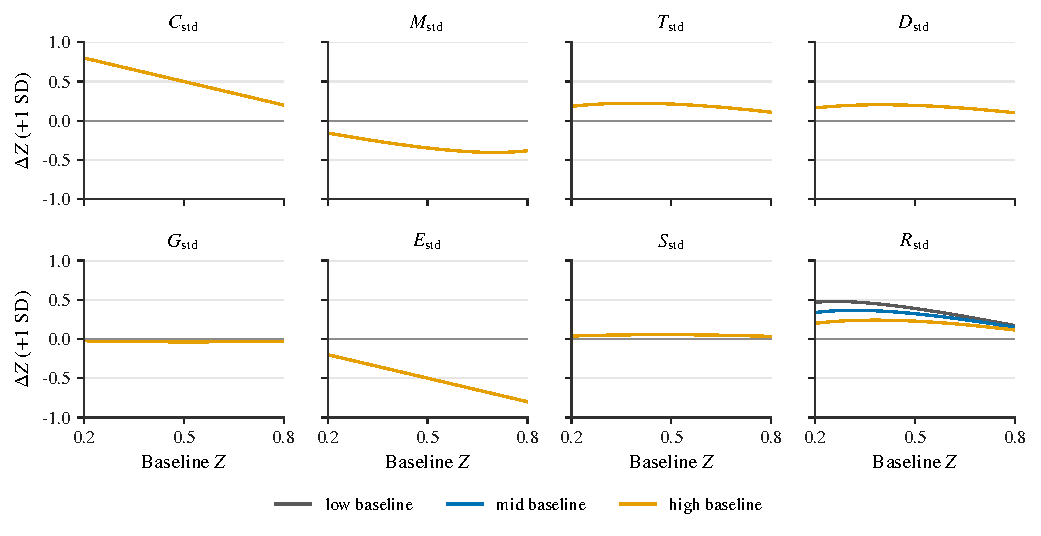
\includegraphics[width=\linewidth]{figure_12_marginal_effect_curves_robust.pdf}
  \caption{\textbf{Data scope:} robustness rendering of the same marginal-effect curves as Fig.~\ref{fig:marginal-effect-curves}, shown on a fixed normalized baseline-$Z$ range $[0.2,0.8]$. \textbf{Method context:} the fixed axis improves readability and visual comparability across modifiers without redefining the empirically supported baseline-$Z$ band used in the main figure. \textbf{Interpretation boundary:} this is a visualization-only robustness view, not a separate inferential family or causal evidence.}\label{fig:marginal_effect_curves_robust}
\end{figure}
\begin{figure}[!htbp]
\centering
\begin{minipage}[t]{0.50\linewidth}%
\vspace{0pt}\centering
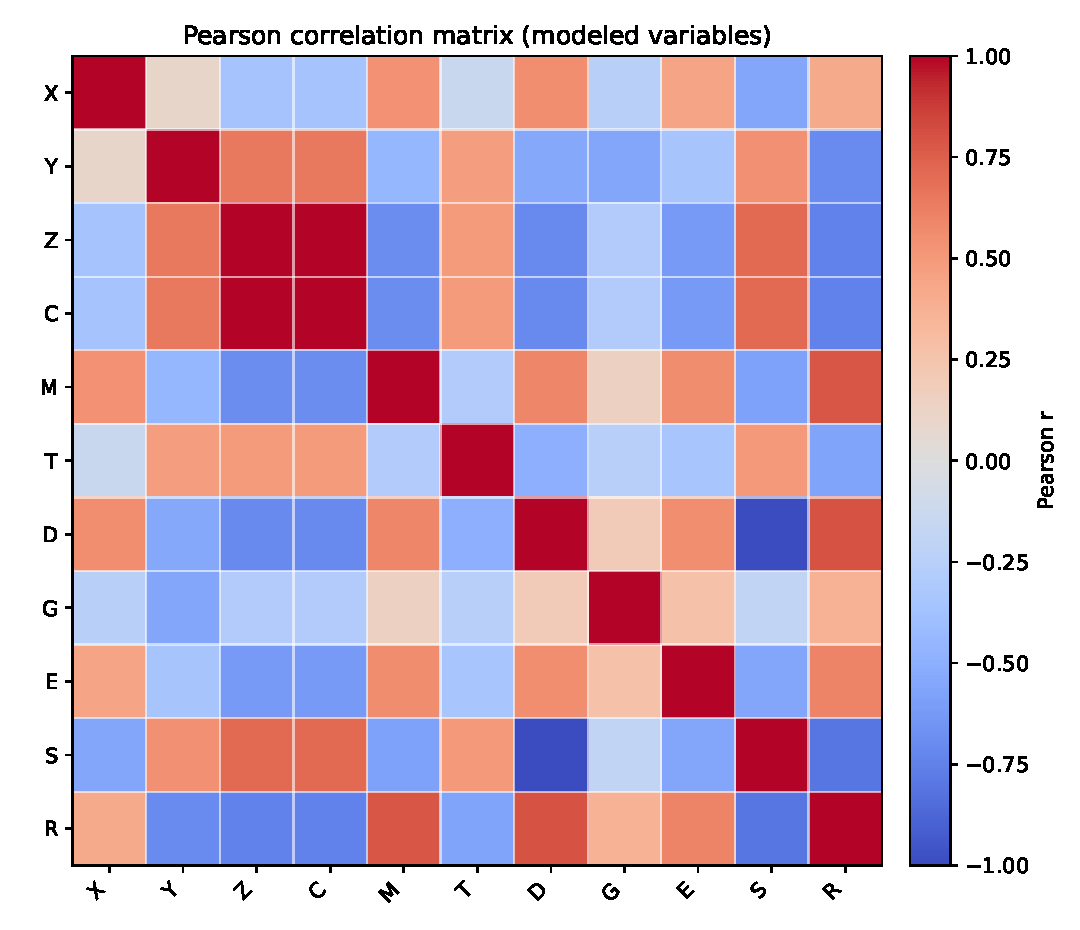
\includegraphics[width=\linewidth]{figure_A2_correlation_heatmap.pdf}
\end{minipage}%
\hspace{0.04\linewidth}%
\begin{minipage}[t]{0.46\linewidth}%
\vspace{0pt}
\captionof{figure}{\textbf{Data scope:} Pearson correlation matrix for the modeled variables on complete-case rows using the same required-column filtering rule as the estimation build step. \textbf{Method context:} the matrix provides a descriptive diagnostic of linear association and potential collinearity in the modeled variable block (generated by \protect\nolinkurl{paper/scripts/make_fig_correlation_heatmap.py}). \textbf{Interpretation boundary:} it is not a validation claim, evidence-tier result, or causal statement.}
\label{fig:correlation}
\end{minipage}
\end{figure}
\noindent\justifying
\textit{Reading note.} The pooled correlation heatmap reflects both between- and within-country dependence structure, whereas the within-country heatmap removes country means and therefore emphasizes co-movement over time within each panel.
This distinction matters for interpretation: strong pooled correlations can be driven by cross-sectional level differences, while within-panel correlations are more indicative of temporal coupling that could confound regime-based narratives.
As a practical check, modifiers that are strongly correlated within-panel should be interpreted with additional caution in the regime-difference tables: large apparent effects may reflect shared temporal dynamics rather than separable mechanisms.
\begin{figure}[!htbp]
  \centering
  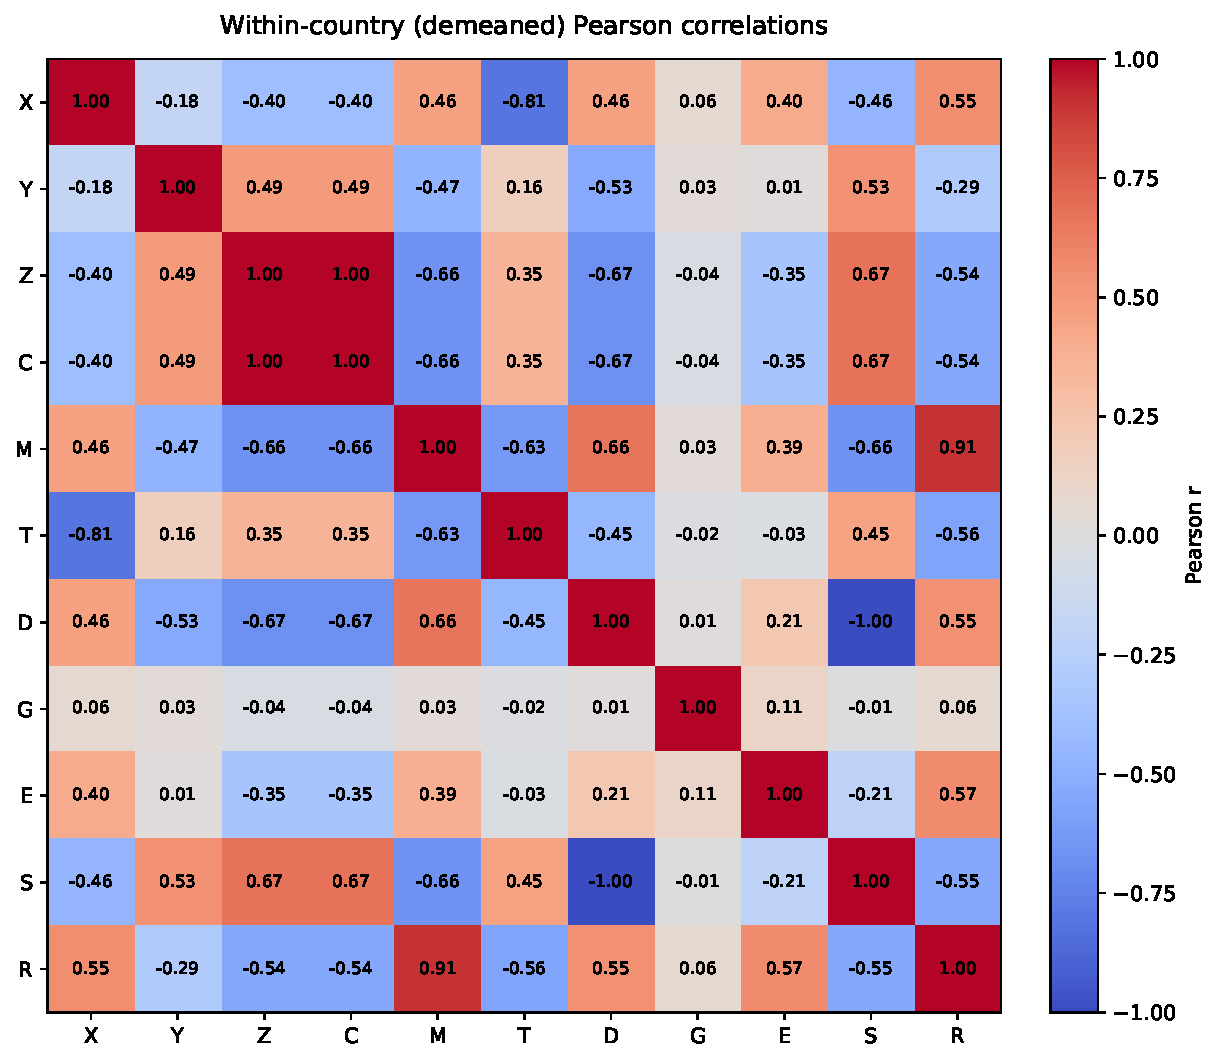
\includegraphics[width=0.72\linewidth]{figure_A3_correlation_heatmap_within.pdf}
  \caption{\textbf{Data scope:} within-country (demeaned) Pearson correlation matrix for the modeled variable block $X,Y,Z,C,M,T,D,G,E,S,R$ on complete-case rows. \textbf{Method context:} demeaning removes country fixed effects to emphasize within-panel dependence structure. \textbf{Interpretation boundary:} this is descriptive context for reading regime narratives and possible confounding, not validation or causal evidence.}
  \label{fig:correlation-within}
\end{figure}
\Section{Reproducibility and additional diagnostics (moved from appendix)}
\noindent\justifying
This block consolidates reproducibility notes and supporting diagnostics that are referenced from the main text as
Figure/Table~S\#. It is included here so the anonymous main manuscript can remain within the journal’s length constraints
without an appendix.

\noindent\justifying
\textbf{Rawdata processing: source-to-column mapping.} The following table provides a compact, auditable mapping
from raw files under \nolinkurl{rawdata/} to the columns they feed in \nolinkurl{rawdata/panel_model_data.csv} and,
where relevant, to the modeled variables. It is included here to support verification of variable provenance.

\begin{table}[!htbp]
\centering
\TableStyle
\caption{\textbf{Data scope:} source\,$\rightarrow$\,column provenance map for the integrated panel (\nolinkurl{rawdata/panel_model_data.csv}). \textbf{Method context:} \textit{Model} indicates which of $X,Y,Z,C,M,T,D,G,E,S,R$ each source contributes to directly or via deterministic transforms, and panel-wide coverage is summarized in \nolinkurl{rawdata/panel_model_data.json}. \textbf{Interpretation boundary:} this is provenance documentation only; it is not inferential evidence or a quality claim by itself.}
\label{tab:source-column-map}
\scriptsize
\setlength{\tabcolsep}{3pt}
\renewcommand{\arraystretch}{1.1}
\begin{tabularx}{\linewidth}{@{}>{\raggedright\arraybackslash}p{0.22\linewidth} >{\raggedright\arraybackslash}p{0.30\linewidth} >{\raggedright\arraybackslash}X >{\raggedright\arraybackslash}p{0.16\linewidth}@{}}
\toprule
Source (rawdata/) & Raw file(s) (as committed) & Contributed columns in panel\_model\_data.csv & Model variables (X,Y,Z,C,M,T,D,G,E,S,R) \\
\midrule
World Values Survey (WVS) constructs & \nolinkurl{rawdata/wvs_combined.csv} (built from WVS/EVS extracts, using \nolinkurl{config/wvs_items.yaml}) & \texttt{Z\_religion\_importance}, \texttt{Z\_violence\_justifiable}, \texttt{Z\_belief\_outcome}, \texttt{C\_religiosity\_index}, \texttt{C\_cultural\_intensity}, \texttt{D\_social\_trust}, \texttt{D\_social\_atomization}, \texttt{S\_support\_index}, \texttt{S\_social\_support}, (plus auxiliary WVS fields) & $Z$, $C$, $D$, $S$ \\
World Bank WDI (macro) & \nolinkurl{rawdata/worldbank_data_new.csv} and WDI bulk exports (\nolinkurl{rawdata/WDICSV.csv}, metadata files) & \texttt{urban\_pop\_share}, \texttt{gdp\_ppp} & $X$ (from \texttt{urban\_pop\_share}) \\
World Bank Internet usage & \nolinkurl{rawdata/worldbank_internet_usage.csv} and API export \nolinkurl{rawdata/API\_IT.NET.USER.ZS\_DS2\_en\_csv\_v2\_280824.csv} & \texttt{internet\_users\_pct} & $M$ (via deterministic standardization to \texttt{M\_media\_environment}) \\
OECD inequality (Gini levels) & \nolinkurl{rawdata/oecd_gini.csv} (derived from OECD WISE/IDD extracts) & \texttt{gini\_index}, \texttt{gini\_disposable} & $Y$ (via deterministic transform to \texttt{Y\_gini}) \\
OECD redistribution scenarios & \nolinkurl{rawdata/oecd_redistribution.csv}, \nolinkurl{rawdata/OECD\_Redistribution\_derived.csv} & \texttt{market\_gini}, \texttt{disposable\_gini}, \texttt{redistribution\_effect}, \texttt{redistribution\_pct} & $G$ (via deterministic transform to \nolinkurl{G_redistribution_capacity}); scenario replication keys \\
OECD SOCX (social spending) & \nolinkurl{rawdata/oecd_socx.csv} (plus \nolinkurl{rawdata/SOCX2025-All-nat-cur.xlsx} as upstream export) & \texttt{socx\_public\_social\_spending\_gdp} & $R$ (via deterministic transform to \texttt{R\_welfare\_capacity}) \\
UNDP Human Development (HDR) & \nolinkurl{rawdata/undp_hdi.csv} (from HDR exports) & \texttt{hdi} & $R$ (via deterministic transform to \texttt{R\_welfare\_capacity}) \\
Education capacity proxy & (as encoded in the integrated panel) & \texttt{sec\_enroll\_gross} & $E$ (via deterministic transform to \nolinkurl{E_education_capacity}) \\
UCDP conflict deaths & \nolinkurl{rawdata/ucdp_conflict_deaths.csv} (plus \nolinkurl{rawdata/GEDEvent\_v25\_1.csv} as upstream export) & \texttt{total\_battle\_deaths} & $T$ (via deterministic transform to \texttt{T\_trauma\_shock}) \\
EM-DAT disasters & \nolinkurl{rawdata/emdat_disasters.csv} (plus public EM-DAT request exports) & \texttt{total\_affected}, \texttt{total\_deaths} & $T$ (via deterministic transform to \texttt{T\_trauma\_shock}) \\
\bottomrule
\end{tabularx}
\end{table}

\noindent\justifying
\textbf{Coefficient artifact key mapping.} The interactive application and the deterministic evaluation scripts use a
single production-pinned coefficient contract encoded in \nolinkurl{src/data/feCoefficients.ts}. The UI can optionally
load an external coefficient artifact at runtime (see the schema in \nolinkurl{src/utils/validation/coefficientsSchema.ts}).
Both sources use the same internal coefficient keys (e.g., \texttt{c1}, \texttt{c\_cm}) while coefficients are reported using
mathematical symbols in Eq.~\eqref{eq:phi}. The table below provides the key-to-symbol mapping.

\begin{table}[!htbp]
\centering
\TableStyle
\caption{\textbf{Data scope:} mapping between internal coefficient keys and the terms used in Eq.~(\ref{eq:phi}). \textbf{Method context:} the table connects the production-pinned coefficient contract in \nolinkurl{src/data/feCoefficients.ts} to manuscript notation so UI, scripts, and paper outputs can be audited against the same artifact names. \textbf{Interpretation boundary:} this is a nomenclature bridge only, not empirical evidence or validation.}
\label{tab:coef-key-map}
\begin{tabular*}{\linewidth}{@{\extracolsep{\fill}}lll@{\hspace{1.5em}}lll@{}}
\toprule
Artifact key & Eq.~(\ref{eq:phi}) & Term & Artifact key & Eq.~(\ref{eq:phi}) & Term \\
\midrule
\texttt{c1} & $c_{C}$ & $C_{\mathrm{std}}$ & \texttt{c\_c2} & $c_{\mathrm{c2}}$ & $C_{\mathrm{std}}^{2}$ \\
\texttt{c2} & $c_{M}$ & $M_{\mathrm{std}}$ & \texttt{c\_m2} & $c_{\mathrm{m2}}$ & $M_{\mathrm{std}}^{2}$ \\
\texttt{c3} & $c_{T}$ & $T_{\mathrm{std}}$ & \texttt{c\_t2} & $c_{\mathrm{t2}}$ & $T_{\mathrm{std}}^{2}$ \\
\texttt{c4} & $c_{D}$ & $D_{\mathrm{std}}$ & \texttt{c\_e2} & $c_{\mathrm{e2}}$ & $E_{\mathrm{std}}^{2}$ \\
\texttt{c5} & $c_{G}$ & $G_{\mathrm{std}}$ & \texttt{alpha} & $\alpha$ & Elasticity on $\log X$ \\
\texttt{c6} & $c_{E}$ & $E_{\mathrm{std}}$ & \texttt{beta} & $\beta$ & Elasticity on $\log Y$ \\
\texttt{c7} & $c_{S}$ & $S_{\mathrm{std}}$ & \texttt{k} & $k$ & Half-saturation constant \\
\texttt{c8} & $c_{R}$ & $R_{\mathrm{std}}$ & \texttt{phi0} & $\phi_{0}$ & Baseline offset \\
\texttt{c\_xy} & $c_{\mathrm{xy}}$ & $X\,Y$ & \multicolumn{3}{c}{} \\
\texttt{c\_yr} & $c_{\mathrm{yr}}$ & $Y\,R_{\mathrm{std}}$ & \multicolumn{3}{c}{} \\
\texttt{c\_tr} & $c_{\mathrm{tr}}$ & $T_{\mathrm{std}}\,R_{\mathrm{std}}$ & \multicolumn{3}{c}{} \\
\texttt{c\_cm} & $c_{\mathrm{cm}}$ & $C_{\mathrm{std}}\,M_{\mathrm{std}}$ & \multicolumn{3}{c}{} \\
\texttt{c\_es} & $c_{\mathrm{es}}$ & $E_{\mathrm{std}}\,S_{\mathrm{std}}$ & \multicolumn{3}{c}{} \\
\texttt{c\_dt} & $c_{\mathrm{dt}}$ & $D_{\mathrm{std}}\,T_{\mathrm{std}}$ & \multicolumn{3}{c}{} \\
\texttt{c\_gr} & $c_{\mathrm{gr}}$ & $G_{\mathrm{std}}\,R_{\mathrm{std}}$ & \multicolumn{3}{c}{} \\
\bottomrule
\end{tabular*}
\end{table}

\noindent\justifying
\textbf{Additional supporting tables.} The following tables document slice-wise evaluation stability and descriptive
collinearity diagnostics under the fixed preprocessing/coefficients contract. These appendixed fixed-model tables are
descriptive diagnostics only and are not part of the primary refit OOS inferential evidence family used for Tier A/B
claims.

\begingroup

\begin{table}[t]
\centering
\TableStyle
\caption{\textbf{Data scope:} fixed-coefficient bounded-scale evaluation metrics by temporal slice. \textbf{Method context:} rows compare all years and three time blocks under the same preprocessing and coefficient contract, with nUsed counting rows with finite observed and predicted $Z$. \textbf{Interpretation boundary:} this table is a descriptive slice diagnostic only; it is not refit OOS evidence or causal support.}
\label{tab:appx-temporal-slice}
{\setlength{\tabcolsep}{1pt}%
\begin{tabularx}{\linewidth}{@{} l >{\raggedright\arraybackslash}X r S[table-format=-1.3] S[table-format=-1.3] S[table-format=-1.4] S[table-format=-1.4] S[table-format=-1.4] S[table-format=-1.4] S[table-format=-1.4] S[table-format=-1.4] @{} }
\toprule
Period & Years & nUsed / nTotal & \multicolumn{1}{c}{$R^{2}$} & \multicolumn{1}{c}{Corr} & \multicolumn{1}{c}{MAE} & \multicolumn{1}{c}{RMSE} & \multicolumn{1}{c}{Bias} & \multicolumn{1}{c}{Residual P10} & \multicolumn{1}{c}{Residual P50} & \multicolumn{1}{c}{Residual P90} \\\\
\midrule
all years & --- & 167 / 167 & 0.252 & 0.577 & 0.1789 & 0.2268 & 0.0611 & -0.1844 & 0.0448 & 0.3196 \\
\ensuremath{\le} 2005 & \ensuremath{\le} 2005 & 45 / 45 & -0.564 & 0.289 & 0.2360 & 0.2851 & 0.1508 & -0.1446 & 0.1804 & 0.4864 \\
2006--2012 & \ensuremath{>} 2005 to \ensuremath{\le} 2012 & 65 / 65 & 0.438 & 0.668 & 0.1816 & 0.2239 & 0.0258 & -0.2254 & -0.0044 & 0.3203 \\
\ensuremath{>} 2012 & \ensuremath{>} 2012 & 57 / 57 & 0.459 & 0.691 & 0.1309 & 0.1715 & 0.0307 & -0.1536 & -0.0139 & 0.2751 \\
\bottomrule
\end{tabularx}
}
\\[0.25em]
{\TableNoteStyle nUsed counts rows with finite observed and predicted Z.}
\end{table}
\endgroup

{\TableStyle
\begin{longtable}{@{} p{0.12\linewidth} r r S[table-format=-1.3] S[table-format=1.4] S[table-format=1.4] S[table-format=-1.4] S[table-format=-1.4] S[table-format=-1.4] S[table-format=-1.4] @{} }
\caption*{\textbf{Data scope:} in-sample bounded-scale evaluation metrics by country slice with no refit. \textbf{Method context:} metrics are computed per country on rows with finite observed and predicted $Z$ under the fixed preprocessing and coefficient contract; em-dashes indicate undefined metrics or sample-size rule failures. \textbf{Interpretation boundary:} this is a descriptive heterogeneity screen only, not Tier A/B refit OOS evidence, transportability, or causal identification.}\\
\toprule
Country & nUsed / nTotal & \multicolumn{1}{c}{$R^{2}$} & \multicolumn{1}{c}{$r$} & \multicolumn{1}{c}{MAE} & \multicolumn{1}{c}{RMSE} & \multicolumn{1}{c}{Bias} & \multicolumn{1}{c}{Residual P10} & \multicolumn{1}{c}{Residual P50} & \multicolumn{1}{c}{Residual P90}\\
\midrule
\endfirsthead
\toprule
Country & nUsed / nTotal & \multicolumn{1}{c}{$R^{2}$} & \multicolumn{1}{c}{$r$} & \multicolumn{1}{c}{MAE} & \multicolumn{1}{c}{RMSE} & \multicolumn{1}{c}{Bias} & \multicolumn{1}{c}{Residual P10} & \multicolumn{1}{c}{Residual P50} & \multicolumn{1}{c}{Residual P90}\\
\midrule
\endhead
\bottomrule
\endfoot
ALL & 167 / 167 & 0.252 & 0.577 & 0.1789 & 0.2268 & 0.0611 & -0.1892 & 0.0284 & 0.3093\\
ARG & 4 / 4 & -0.251 & 0.620 & 0.0919 & 0.1124 & 0.0059 & -0.0811 & -0.0416 & 0.1309\\
MEX & 4 / 4 & 0.143 & 0.520 & 0.1113 & 0.1324 & -0.0208 & -0.1432 & -0.0399 & 0.1169\\
PER & 4 / 4 & -0.090 & 0.557 & 0.0944 & 0.1243 & 0.0339 & -0.0612 & -0.0171 & 0.1699\\
CAN & 3 / 3 & 0.086 & 0.607 & 0.1419 & 0.1579 & -0.0540 & -0.1974 & -0.0628 & 0.0930\\
DEU & 3 / 3 & -32.744 & -0.685 & 0.1481 & 0.1567 & 0.1481 & 0.0979 & 0.1480 & 0.1983\\
ESP & 3 / 3 & -5.766 & 0.998 & 0.1263 & 0.1333 & 0.1263 & 0.0856 & 0.1219 & 0.1687\\
IDN & 3 / 3 & -0.945 & 0.916 & 0.1423 & 0.1855 & -0.1423 & -0.2632 & -0.0823 & -0.0454\\
ROU & 3 / 3 & -1.135 & 0.999 & 0.1860 & 0.2062 & -0.1860 & -0.2767 & -0.1526 & -0.1086\\
RUS & 3 / 3 & -351.272 & -0.435 & 0.1768 & 0.2023 & 0.1768 & 0.0935 & 0.1344 & 0.2770\\
THA & 3 / 3 & 0.323 & 0.787 & 0.2013 & 0.2084 & 0.0785 & -0.1183 & 0.1459 & 0.2482\\
TUR & 3 / 3 & -0.849 & 0.843 & 0.1514 & 0.1679 & -0.1514 & -0.2076 & -0.1938 & -0.0782\\
UKR & 3 / 3 & -4.251 & 1.000 & 0.0756 & 0.0852 & 0.0756 & 0.0368 & 0.0773 & 0.1137\\
BRA & 2 / 2 & \textemdash{} & 1.000 & 0.0623 & 0.0704 & -0.0623 & -0.0886 & -0.0623 & -0.0360\\
CHL & 2 / 2 & \textemdash{} & -1.000 & 0.1639 & 0.1643 & 0.0122 & -0.1189 & 0.0122 & 0.1433\\
COL & 2 / 2 & \textemdash{} & 1.000 & 0.0156 & 0.0169 & -0.0156 & -0.0207 & -0.0156 & -0.0106\\
ECU & 2 / 2 & \textemdash{} & 1.000 & 0.0327 & 0.0378 & -0.0327 & -0.0479 & -0.0327 & -0.0176\\
GEO & 2 / 2 & \textemdash{} & 1.000 & 0.1213 & 0.1281 & -0.1213 & -0.1543 & -0.1213 & -0.0882\\
KAZ & 2 / 2 & \textemdash{} & -1.000 & 0.0975 & 0.1097 & 0.0503 & -0.0277 & 0.0503 & 0.1283\\
KGZ & 2 / 2 & \textemdash{} & 1.000 & 0.2963 & 0.2966 & 0.2963 & 0.2852 & 0.2963 & 0.3073\\
KOR & 2 / 2 & \textemdash{} & 1.000 & 0.0496 & 0.0647 & 0.0496 & 0.0163 & 0.0496 & 0.0828\\
MYS & 2 / 2 & \textemdash{} & 1.000 & 0.2232 & 0.2420 & -0.2232 & -0.2979 & -0.2232 & -0.1484\\
NGA & 2 / 2 & \textemdash{} & 1.000 & 0.0845 & 0.0845 & -0.0845 & -0.0864 & -0.0845 & -0.0826\\
NLD & 2 / 2 & \textemdash{} & 1.000 & 0.2162 & 0.2171 & 0.2162 & 0.2002 & 0.2162 & 0.2321\\
POL & 2 / 2 & \textemdash{} & 1.000 & 0.3085 & 0.3343 & -0.3085 & -0.4117 & -0.3085 & -0.2053\\
ALB & 1 / 1 & \textemdash{} & \textemdash{} & 0.3439 & 0.3439 & 0.3439 & 0.3439 & 0.3439 & 0.3439\\
AUS & 1 / 1 & \textemdash{} & \textemdash{} & 0.0036 & 0.0036 & -0.0036 & -0.0036 & -0.0036 & -0.0036\\
BGR & 1 / 1 & \textemdash{} & \textemdash{} & 0.2369 & 0.2369 & 0.2369 & 0.2369 & 0.2369 & 0.2369\\
CHE & 1 / 1 & \textemdash{} & \textemdash{} & 0.0737 & 0.0737 & -0.0737 & -0.0737 & -0.0737 & -0.0737\\
CHN & 1 / 1 & \textemdash{} & \textemdash{} & 0.7084 & 0.7084 & 0.7084 & 0.7084 & 0.7084 & 0.7084\\
CYP & 1 / 1 & \textemdash{} & \textemdash{} & 0.1446 & 0.1446 & -0.1446 & -0.1446 & -0.1446 & -0.1446\\
CZE & 1 / 1 & \textemdash{} & \textemdash{} & 0.3367 & 0.3367 & 0.3367 & 0.3367 & 0.3367 & 0.3367\\
EST & 1 / 1 & \textemdash{} & \textemdash{} & 0.2169 & 0.2169 & 0.2169 & 0.2169 & 0.2169 & 0.2169\\
FIN & 1 / 1 & \textemdash{} & \textemdash{} & 0.0452 & 0.0452 & 0.0452 & 0.0452 & 0.0452 & 0.0452\\
FRA & 1 / 1 & \textemdash{} & \textemdash{} & 0.3889 & 0.3889 & 0.3889 & 0.3889 & 0.3889 & 0.3889\\
GBR & 1 / 1 & \textemdash{} & \textemdash{} & 0.0448 & 0.0448 & 0.0448 & 0.0448 & 0.0448 & 0.0448\\
GHA & 1 / 1 & \textemdash{} & \textemdash{} & 0.0578 & 0.0578 & 0.0578 & 0.0578 & 0.0578 & 0.0578\\
GRC & 1 / 1 & \textemdash{} & \textemdash{} & 0.1769 & 0.1769 & -0.1769 & -0.1769 & -0.1769 & -0.1769\\
IRN & 1 / 1 & \textemdash{} & \textemdash{} & 0.1501 & 0.1501 & -0.1501 & -0.1501 & -0.1501 & -0.1501\\
ITA & 1 / 1 & \textemdash{} & \textemdash{} & 0.3037 & 0.3037 & -0.3037 & -0.3037 & -0.3037 & -0.3037\\
JPN & 1 / 1 & \textemdash{} & \textemdash{} & 0.1321 & 0.1321 & 0.1321 & 0.1321 & 0.1321 & 0.1321\\
PAK & 1 / 1 & \textemdash{} & \textemdash{} & 0.0618 & 0.0618 & -0.0618 & -0.0618 & -0.0618 & -0.0618\\
SRB & 1 / 1 & \textemdash{} & \textemdash{} & 0.1225 & 0.1225 & 0.1225 & 0.1225 & 0.1225 & 0.1225\\
SVK & 1 / 1 & \textemdash{} & \textemdash{} & 0.1088 & 0.1088 & 0.1088 & 0.1088 & 0.1088 & 0.1088\\
SVN & 1 / 1 & \textemdash{} & \textemdash{} & 0.2245 & 0.2245 & 0.2245 & 0.2245 & 0.2245 & 0.2245\\
URY & 1 / 1 & \textemdash{} & \textemdash{} & 0.0868 & 0.0868 & 0.0868 & 0.0868 & 0.0868 & 0.0868\\
USA & 1 / 1 & \textemdash{} & \textemdash{} & 0.1191 & 0.1191 & -0.1191 & -0.1191 & -0.1191 & -0.1191\\
UZB & 1 / 1 & \textemdash{} & \textemdash{} & 0.0573 & 0.0573 & -0.0573 & -0.0573 & -0.0573 & -0.0573\\
VNM & 1 / 1 & \textemdash{} & \textemdash{} & 0.3087 & 0.3087 & 0.3087 & 0.3087 & 0.3087 & 0.3087\\
\end{longtable}
\par\vspace{0.25em}
{\TableNoteStyle Computed per country on rows with finite observed and predicted Z; no refit (fixed coefficients unless an estimated set is active). Countries with fewer than 30 valid observations may display \enquote{\textemdash{}} due to insufficient sample size. nUsed counts rows with finite observed and predicted Z. Values are shown as \enquote{\textemdash{}} when metrics are undefined or when the minimum per-country sample-size rule applies (e.g., nUsed $<$ 30).}
}
\addtocounter{table}{-1}%--- undo silent longtable counter increment (country-slice table is unnumbered)
\begin{table}[!htbp]
\centering
\TableStyle
\caption{\textbf{Data scope:} variance-inflation-factor diagnostics for the six retained covariates on the complete-case estimation rows ($n=\num{167}$). \textbf{Method context:} $\mathrm{VIF}_j = 1/(1-R_j^2)$, where $R_j^2$ comes from regressing covariate $j$ on the other five; the condition number is that of the design matrix with intercept. Values are emitted by \texttt{generate:collinearity}, not transcribed. \textbf{Interpretation boundary:} this is stability context for reading coefficient signs, not evidence of causal structure; a VIF above the conventional threshold of five describes association under a fixed design rather than a separately identified effect.}
\label{tab:appx-vif}
\begin{tabular}{@{}lrr@{}}
\toprule
Variable & $R^2$ on other covariates & VIF \\
\midrule
$R$ (welfare capacity) & 0.8911 & \num{9.19} \\
$E$ (education capacity) & 0.7892 & \num{4.74} \\
$X$ (urbanization) & 0.6766 & \num{3.09} \\
$M$ (media environment) & 0.6153 & \num{2.60} \\
$Y$ (inequality) & 0.3037 & \num{1.44} \\
$T$ (trauma/shock) & 0.0741 & \num{1.08} \\
\midrule
\multicolumn{3}{@{}l@{}}{\footnotesize Condition number of the design matrix: \num{24.01}} \\
\bottomrule
\end{tabular}
\\[0.35em]
{\TableNoteStyle Two covariates sit high: $R$ at \num{9.19} and $E$ at \num{4.74}. The reason is substantive rather than statistical. $R$ is an affine rescaling of the Human Development Index, $R = 7.303771\,\mathrm{HDI} - 6.005361$ (max residual $0.000000$ over \num{13441} rows), and HDI is itself built partly from education; $E$ is gross secondary enrolment. The two channels therefore share a component by construction. Coefficients on $R$ and $E$ are reported as conditional associations under this design, and no claim in the paper rests on separating their individual contributions. The remaining four covariates are well separated, with $T$ effectively orthogonal ($\mathrm{VIF}=\num{1.08}$).}
\end{table}
\Section{Visual analytics tooling (dashboard, pinned inspection, export contract)}
\noindent\justifying
The following UI and workflow figures document the inspection surface used in the study: how regimes are
explored, how local sensitivity is pinned and compared, and how deterministic PDF exports preserve a
reproducible mapping from UI state to evidence bundles. These figures provide transparency into the interactive analysis process and demonstrate how the computational model is operationalized for scientific inspection. Interactive visual analytics are central to modern quantitative social science, enabling researchers to rapidly explore parameter space, test hypotheses, and communicate findings with supporting evidence.
\noindent\justifying
The dashboard surfaces the decomposition of $\Phi$ and derived quantities, enabling pinned inspection of local states
and side-by-side sensitivity comparison at identical parameter snapshots. A schema-versioned export workflow serializes
the interactive state vector and renderer configuration, guaranteeing that visual artifacts are exactly reproducible.
This audit trail bridges interactive exploration and paper-consistent, deterministic exports. The dashboard visualization (Figure in this section) shows the main inspection interface, while the pinned inspection figure demonstrates how two states are compared side-by-side, and the export workflow figure documents the serialization process that ensures reproducibility of all generated figures. Maintaining a complete audit trail enables other researchers to replicate, verify, or extend the analyses from first principles.

\begin{figure}[!htbp]
  \centering
  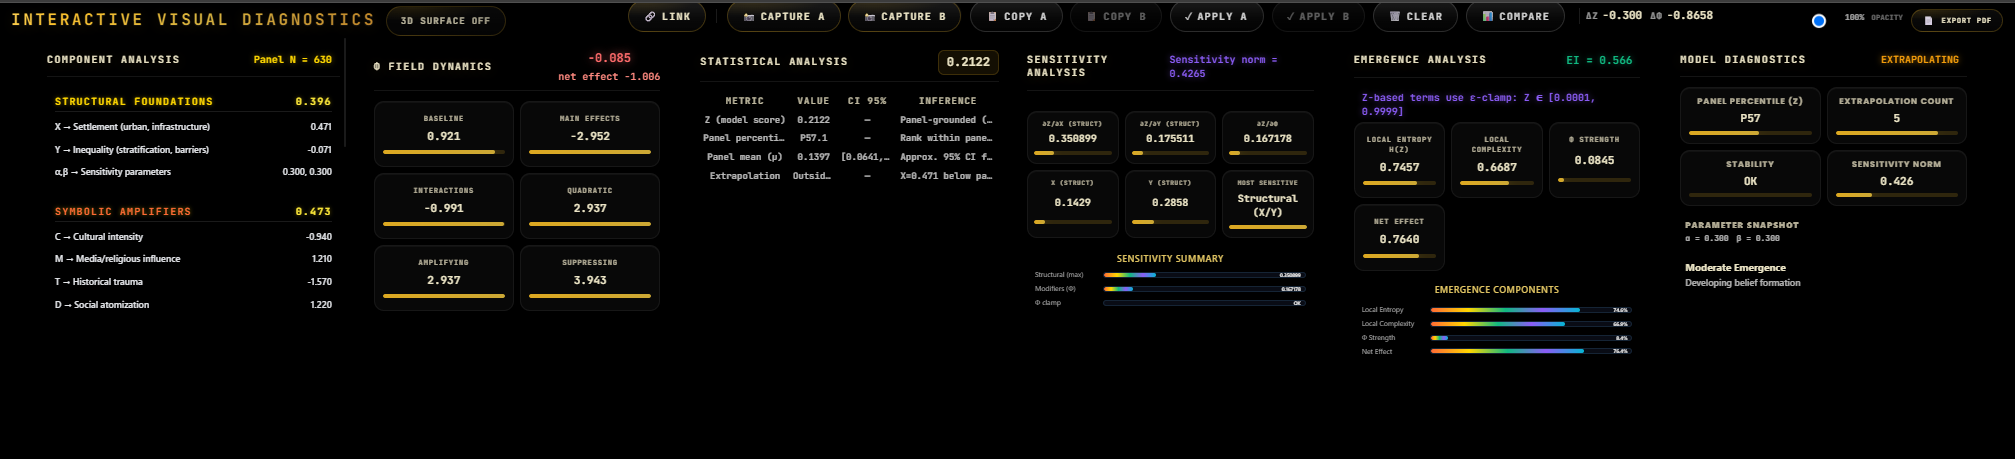
\includegraphics[width=\linewidth]{figure_7_ui_dashboard.png}%
  \caption{\textbf{Data scope:} overview screenshot of the interactive visual analytics dashboard. \textbf{Method context:} the interface documents bounded-transform surface exploration, pinned/slice-based inspection, and deterministic export under the same numerical safety contract used in production. \textbf{Interpretation boundary:} this is a provenance screenshot only; it is not inferential evidence and does not substitute for manuscript evaluation figures.}
  \label{fig:ui-dashboard}
\end{figure}

\begin{figure}[!htbp]
  \begin{minipage}[t]{0.48\linewidth}
    \vspace{0pt}
    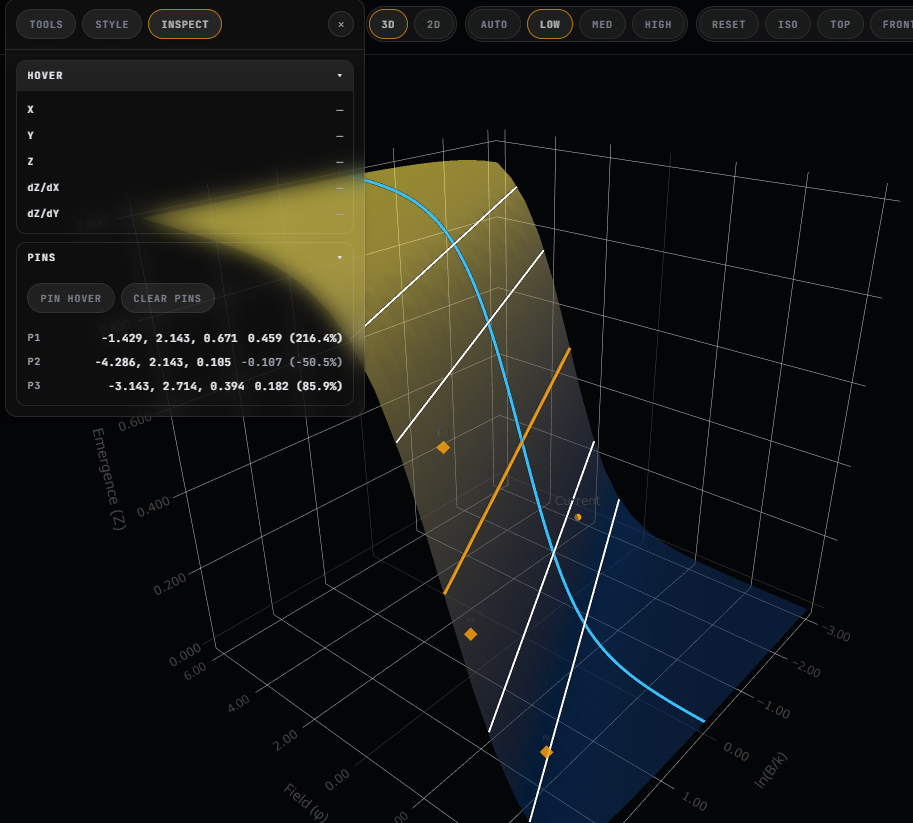
\includegraphics[width=\linewidth]{figure_8_ui_pinned_inspection.png}%
  \end{minipage}\hfill
  \begin{minipage}[t]{0.48\linewidth}
    \vspace{0pt}
    \captionsetup{type=figure, position=top, justification=justified, singlelinecheck=false, skip=2pt}
    \captionof{figure}{\textbf{Data scope:} screenshot of local pinned-point inspection on the 3D response surface. \textbf{Method context:} the UI exposes pinned coordinates, local predicted levels, gradient components, and regime labels for a fixed state under the deterministic contract, allowing pointwise comparison of local sensitivity on the bounded surface. \textbf{Interpretation boundary:} this is provenance and inspection-interface documentation only; it aids local explanation but is not Tier A/B evidence or causal identification.}
    \label{fig:surface-pinned-inspection}
  \end{minipage}
\end{figure}
\noindent\justifying
\textit{Reading note.} Pinned inspection and export are treated as linked components of the evidence workflow: pinning defines the exact coordinates in $(\Phi,s)$ (and UI state vector) that a claim refers to, and exporting makes that state portable.
This reduces the risk of ``unrecorded'' interactive choices when translating exploratory visual analytics into publication-grade figures.
In methodological terms, the pair enforces a provenance constraint: every visual claim is anchored to a concrete state vector that can be replayed and verified by a third party.

\begin{figure}[!htbp]
  \begin{minipage}[t]{0.60\linewidth}
    \vspace{0pt}
    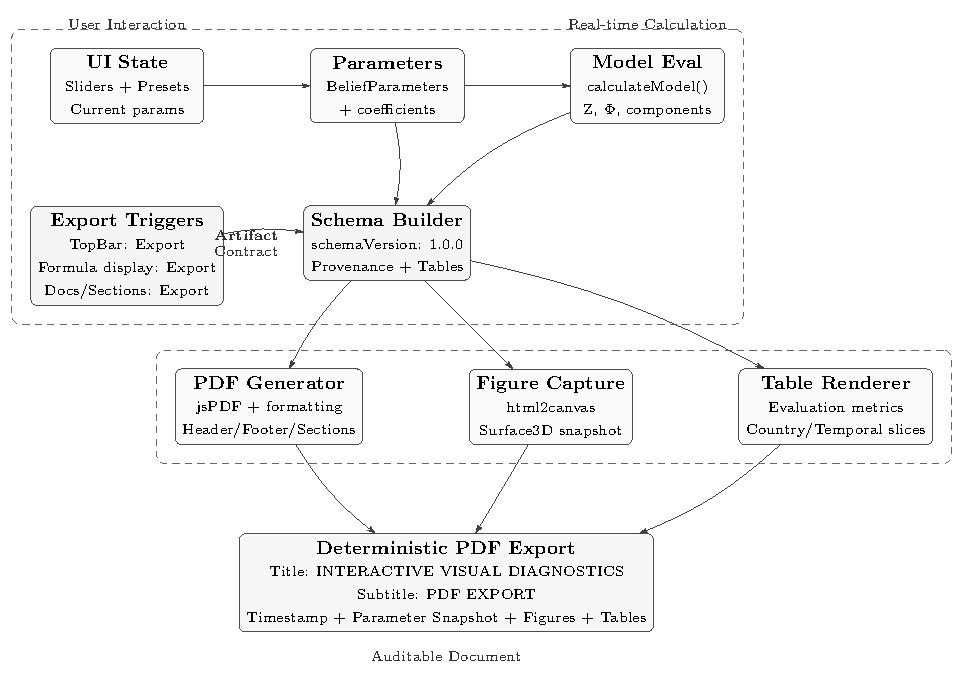
\includegraphics[width=\linewidth]{fig_pdf_export_workflow.pdf}%
  \end{minipage}\hfill
  \begin{minipage}[t]{0.38\linewidth}
    \vspace{0pt}
    \captionsetup{type=figure, position=top, justification=justified, singlelinecheck=false, skip=2pt}
    \captionof{figure}{\textbf{Data scope:} schematic of the PDF export workflow from UI state to compiled artifact. \textbf{Method context:} the export routine serializes a schema-versioned state snapshot that parameterizes downstream renderers while reusing fixed estimation artifacts, preserving the mapping between interactive state and report content. \textbf{Interpretation boundary:} this is a reproducibility-contract figure only; it is not model validation or inferential evidence.}
    \label{fig:pdf-export-workflow}
  \end{minipage}
\end{figure}
\noindent\justifying
\textit{Export contract and reproducibility.} The export workflow serializes the complete interactive state vector (preprocessing bounds, coefficient bundle, pinned inspection coordinates, and renderer options) under a schema-versioned contract. Each PDF export is accompanied by a deterministic snapshot and a metadata header (state hash and schema version) so that regenerated artifacts are bitwise-identical to the original evidence. This design separates (i) the statistical model and bounded map $Z=\sigma(\Phi+s)$ from (ii) the inspection UI, while making the bridge between them auditable. As a result, any figure shown in this supplementary file can be reproduced from the same snapshot without relying on hidden UI conditions.
\Section{Supplementary UI screenshots (additional evidence snapshots)}
\noindent\justifying
These screenshots provide supporting context for the interactive analysis environment. They are included
as an audit trail of UI state and diagnostic panels; \emph{no resizing is applied} beyond the manuscript’s
standard \texttt{width=\string\linewidth} convention. Each screenshot captures a distinct operational state of the interactive system, documenting how the model parameters, decomposition, and derived diagnostics are presented to analysts during the exploration process.
\noindent\justifying
Screenshots are included to document representative parameter states and diagnostic panels, complementing the
main evaluation by showing how the mechanism-level decomposition and checks appear within the analysis surface.
They do not alter the computational contract; rather, they provide additional, verifiable context for the
interpretation pipeline and export protocol. The first screenshots show alternative UI states, followed by explanatory paragraphs describing key inspection techniques (geometry reading, curvature visualization, preset management), and ending with screenshots of specialized diagnostic panels (belief equation, core variables, amplifiers, suppressors, mathematical analysis, system dynamics, and AI interpretation layer).
\noindent\justifying
Transparency in analytical methods is a cornerstone of reproducible science. Documenting the interactive UI state, parameter values, and diagnostic outputs enables readers to understand not just the final conclusions but the entire process by which results were obtained. The screenshots serve as a visual record of the analytical workflow, from initial parameter setting through iterative sensitivity exploration to final evidence generation. This comprehensive documentation supports scientific scrutiny and allows future researchers to build upon the methodology with full confidence in the computational integrity of the reported results.
\noindent\justifying
The following screenshots have been selected to represent key operational states of the analysis UI. Each screenshot is accompanied by technical captions describing the analytical purpose and the displayed diagnostics.
\noindent\justifying
\textit{Reading note.} The primary interpretive role of these screenshots is provenance rather than persuasion: they document what an analyst could see at the time a state was pinned and exported.
Accordingly, the captions focus on the bounded-scale contract, the decomposition of $\Phi$, and the mechanisms used to prevent misreading saturation regions as substantive regime shifts.
In combination with the deterministic export workflow, the screenshots also clarify where a given narrative came from: the key objects are (i) the state vector, (ii) the term-by-term $\Phi$ contributions, and (iii) the bounded-scale sensitivity at that state.
This is intended to make reviewer verification feasible even without re-running interactive exploration from scratch.
Because screenshots are ``thick'' evidence (they embed multiple panels at once), short interpretive guidance is included between blocks to indicate which parts of the UI correspond to which scientific checks (sensitivity, decomposition, and calibration).
\begin{figure}[!htbp]
    \centering
    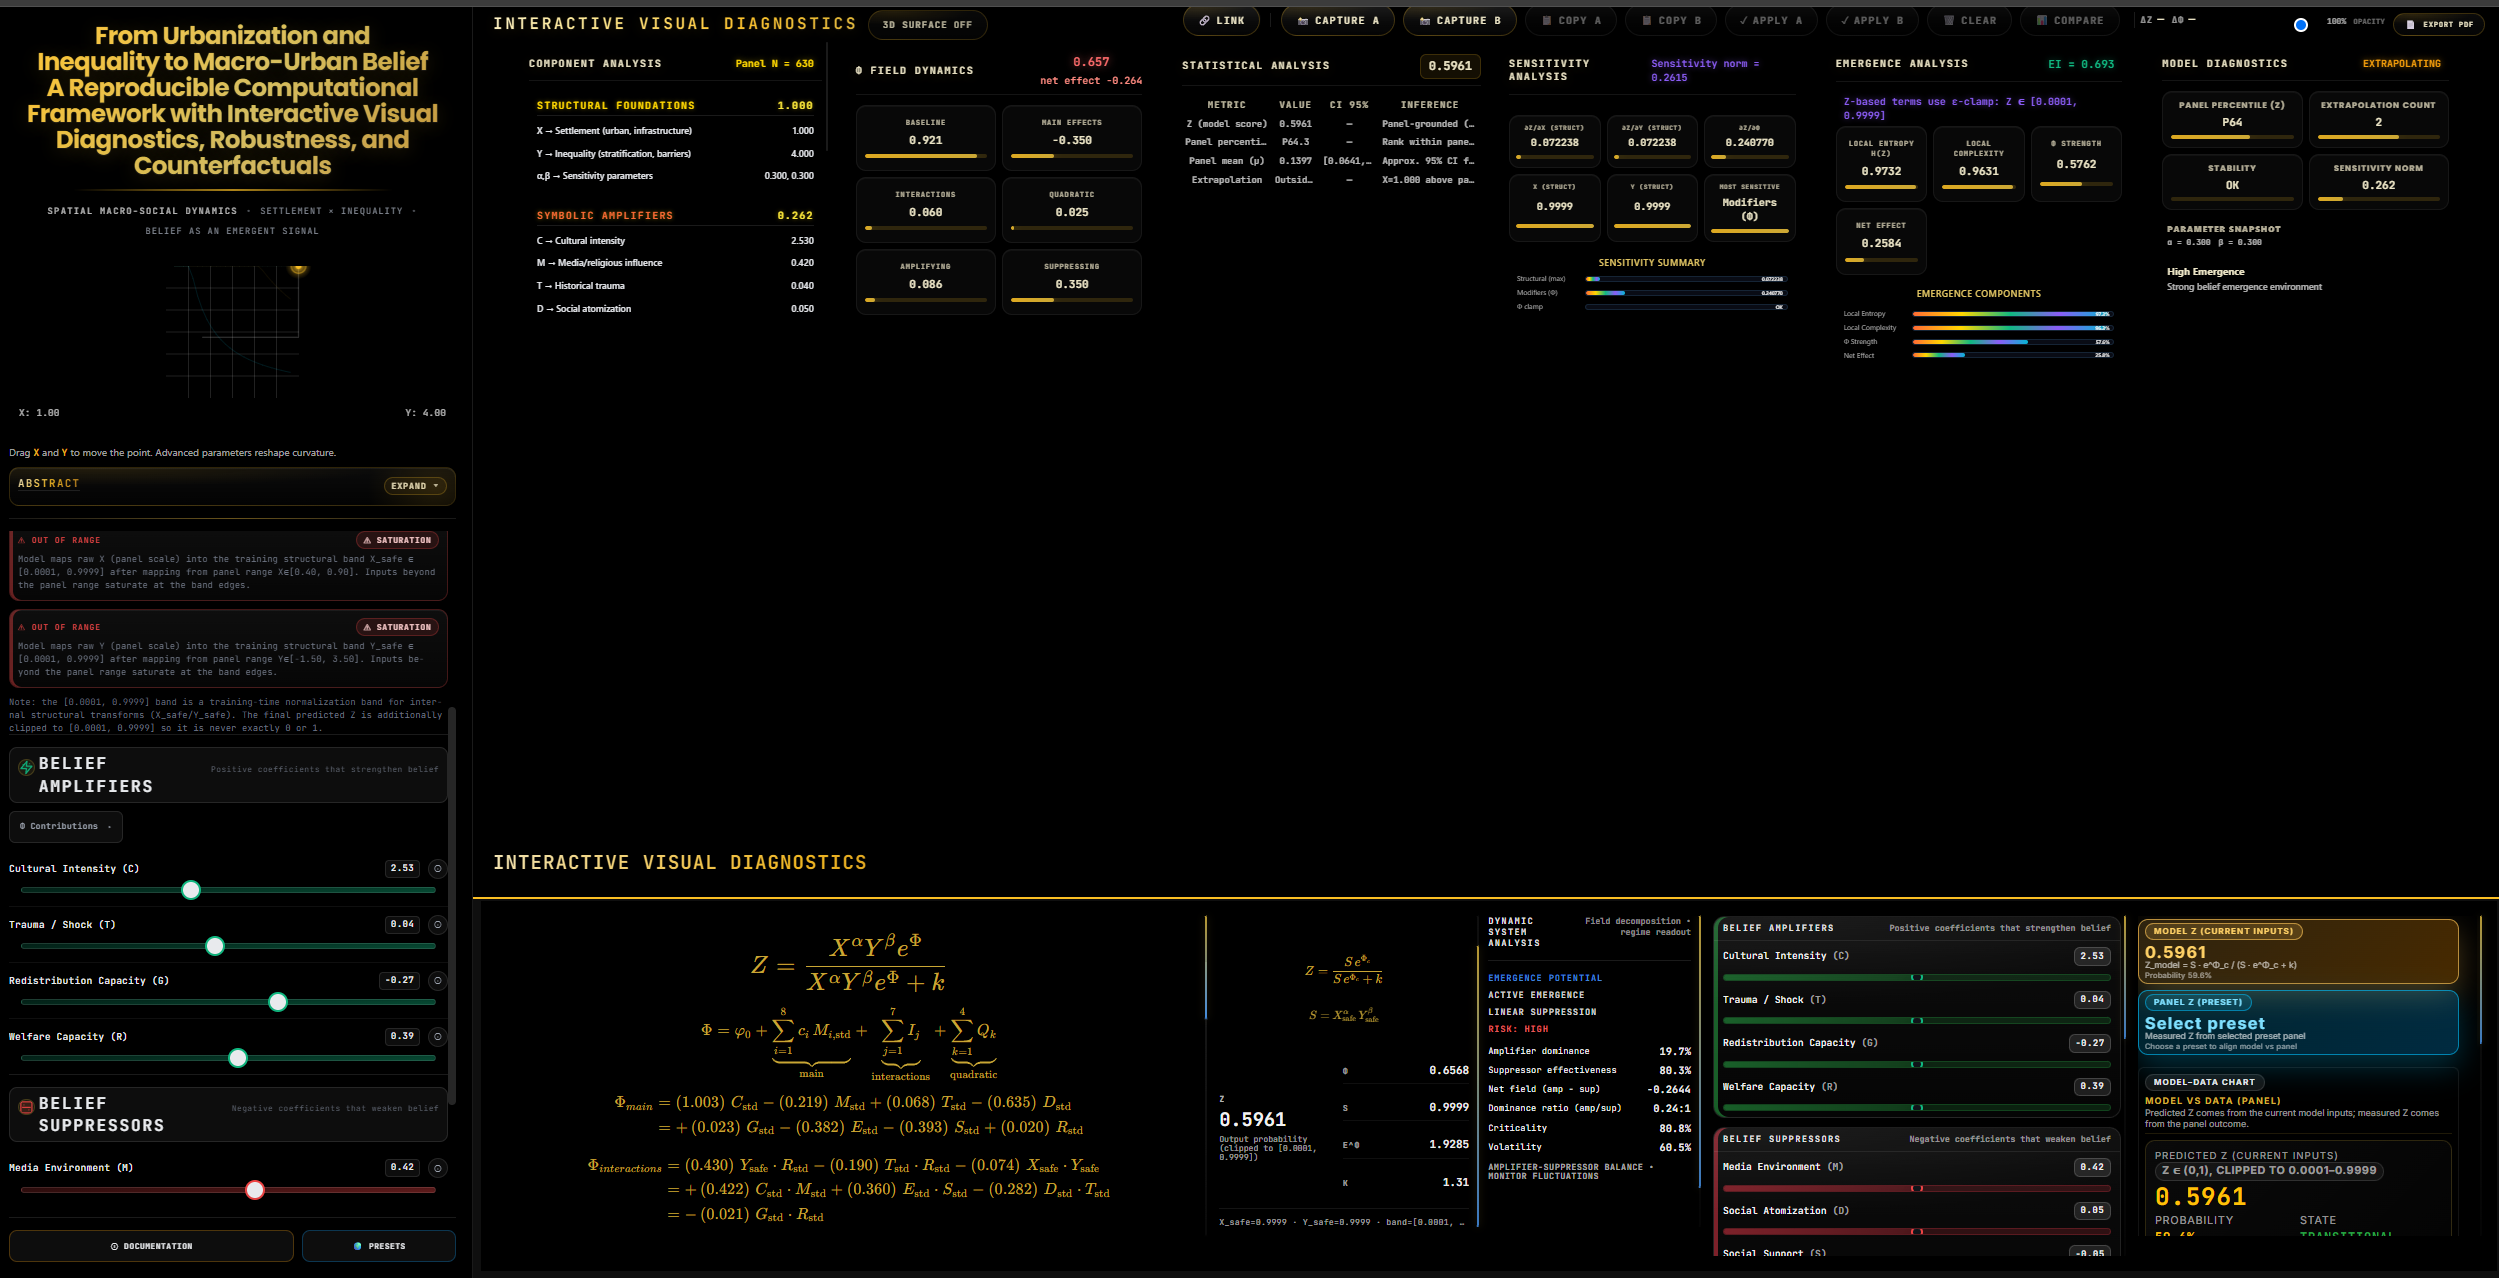
\includegraphics[width=\linewidth]{figure_A4_ui_screenshot_1.png}
    \caption{\textbf{Data scope:} supplementary UI screenshot showing one alternative interactive state snapshot. \textbf{Method context:} the view records a concrete slider/configuration state used to inspect regime dependence of the bounded response $Z$ under the fixed preprocessing and coefficient contracts. \textbf{Interpretation boundary:} this is a provenance screenshot only, included for auditability rather than inferential evidence or causal support.}
\end{figure}
\begin{figure}[!htbp]
    \centering
    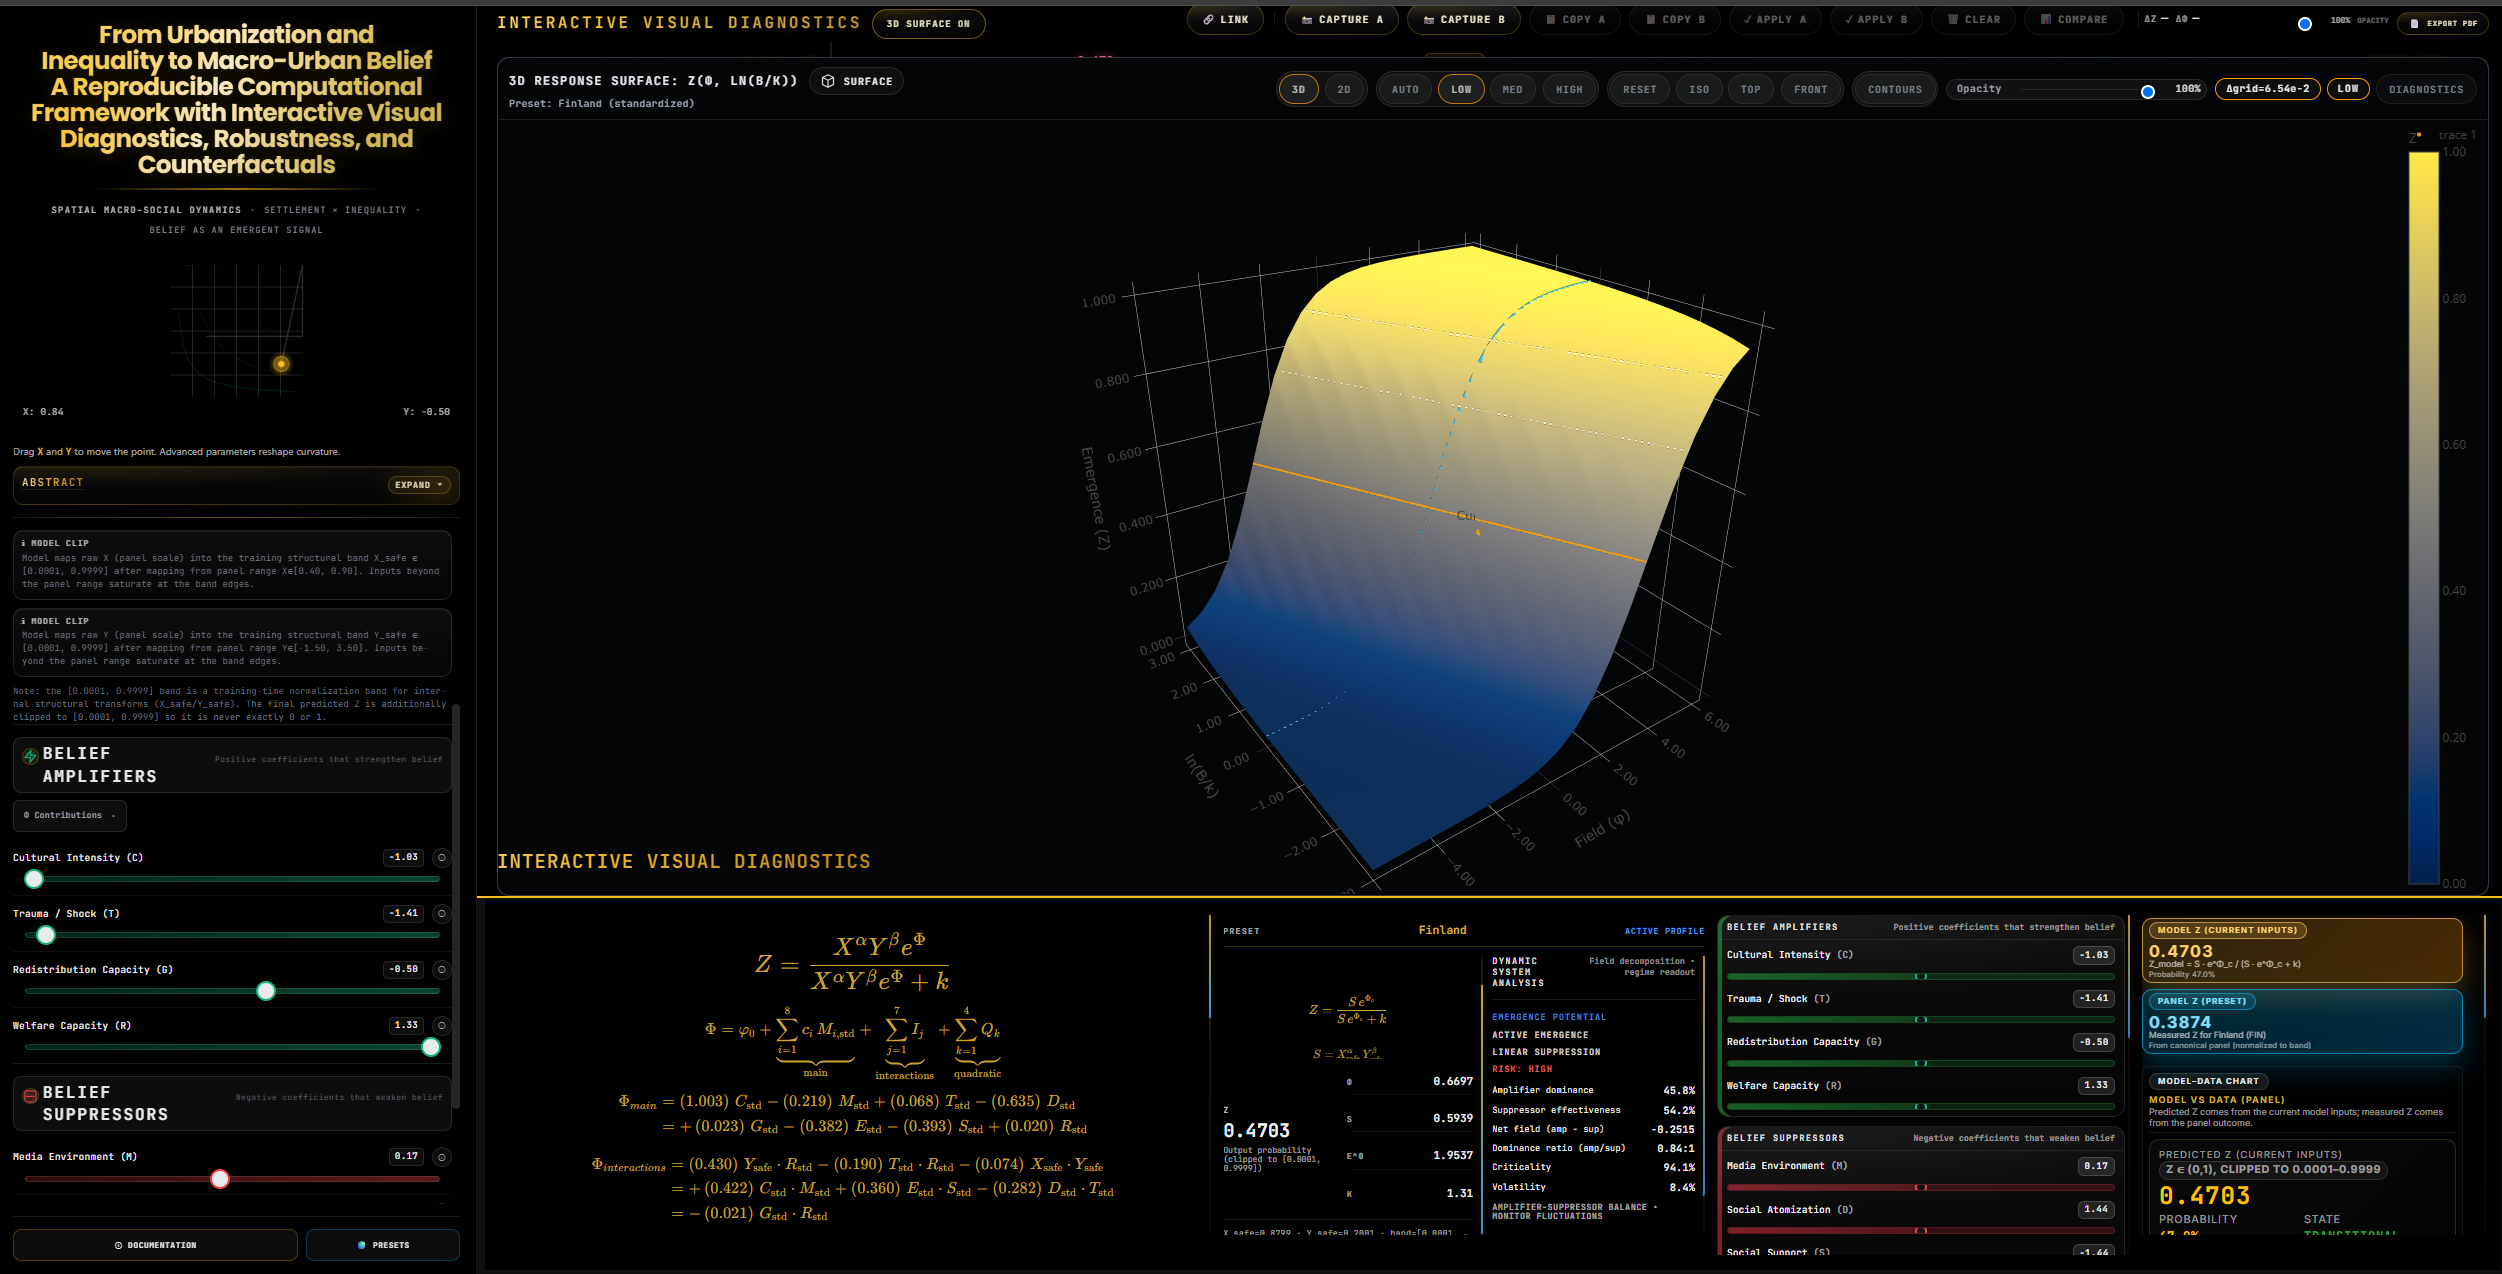
\includegraphics[width=\linewidth]{figure_A5_ui_screenshot_2.png}
    \caption{\textbf{Data scope:} supplementary UI screenshot showing a second interactive state snapshot. \textbf{Method context:} it documents a distinct configuration of controls, surface view, and derived diagnostics under the same preprocessing and coefficient contracts. \textbf{Interpretation boundary:} this is provenance documentation only; it enables replay of the displayed state but does not provide inferential evidence.}
\end{figure}
\noindent\justifying
\textit{Reading the geometry view.} The geometry surface displays the bounded response $Z$ across the $(X,Y)$ stimulus plane under a fixed contextual backdrop, with slices and overlays indicating curvature and sensitivity bands. Because $Z$ is the monotone transform of $\Phi$, apparent slope and saturation reflect local field intensity rather than raw additive scale. Pinned inspection compares two states with identical preprocessing and coefficients, isolating the effect of baseline shifts; this makes regime-dependent differences interpretable without conflating them with scaling artefacts.
\begin{figure}[!htbp]
    \centering
    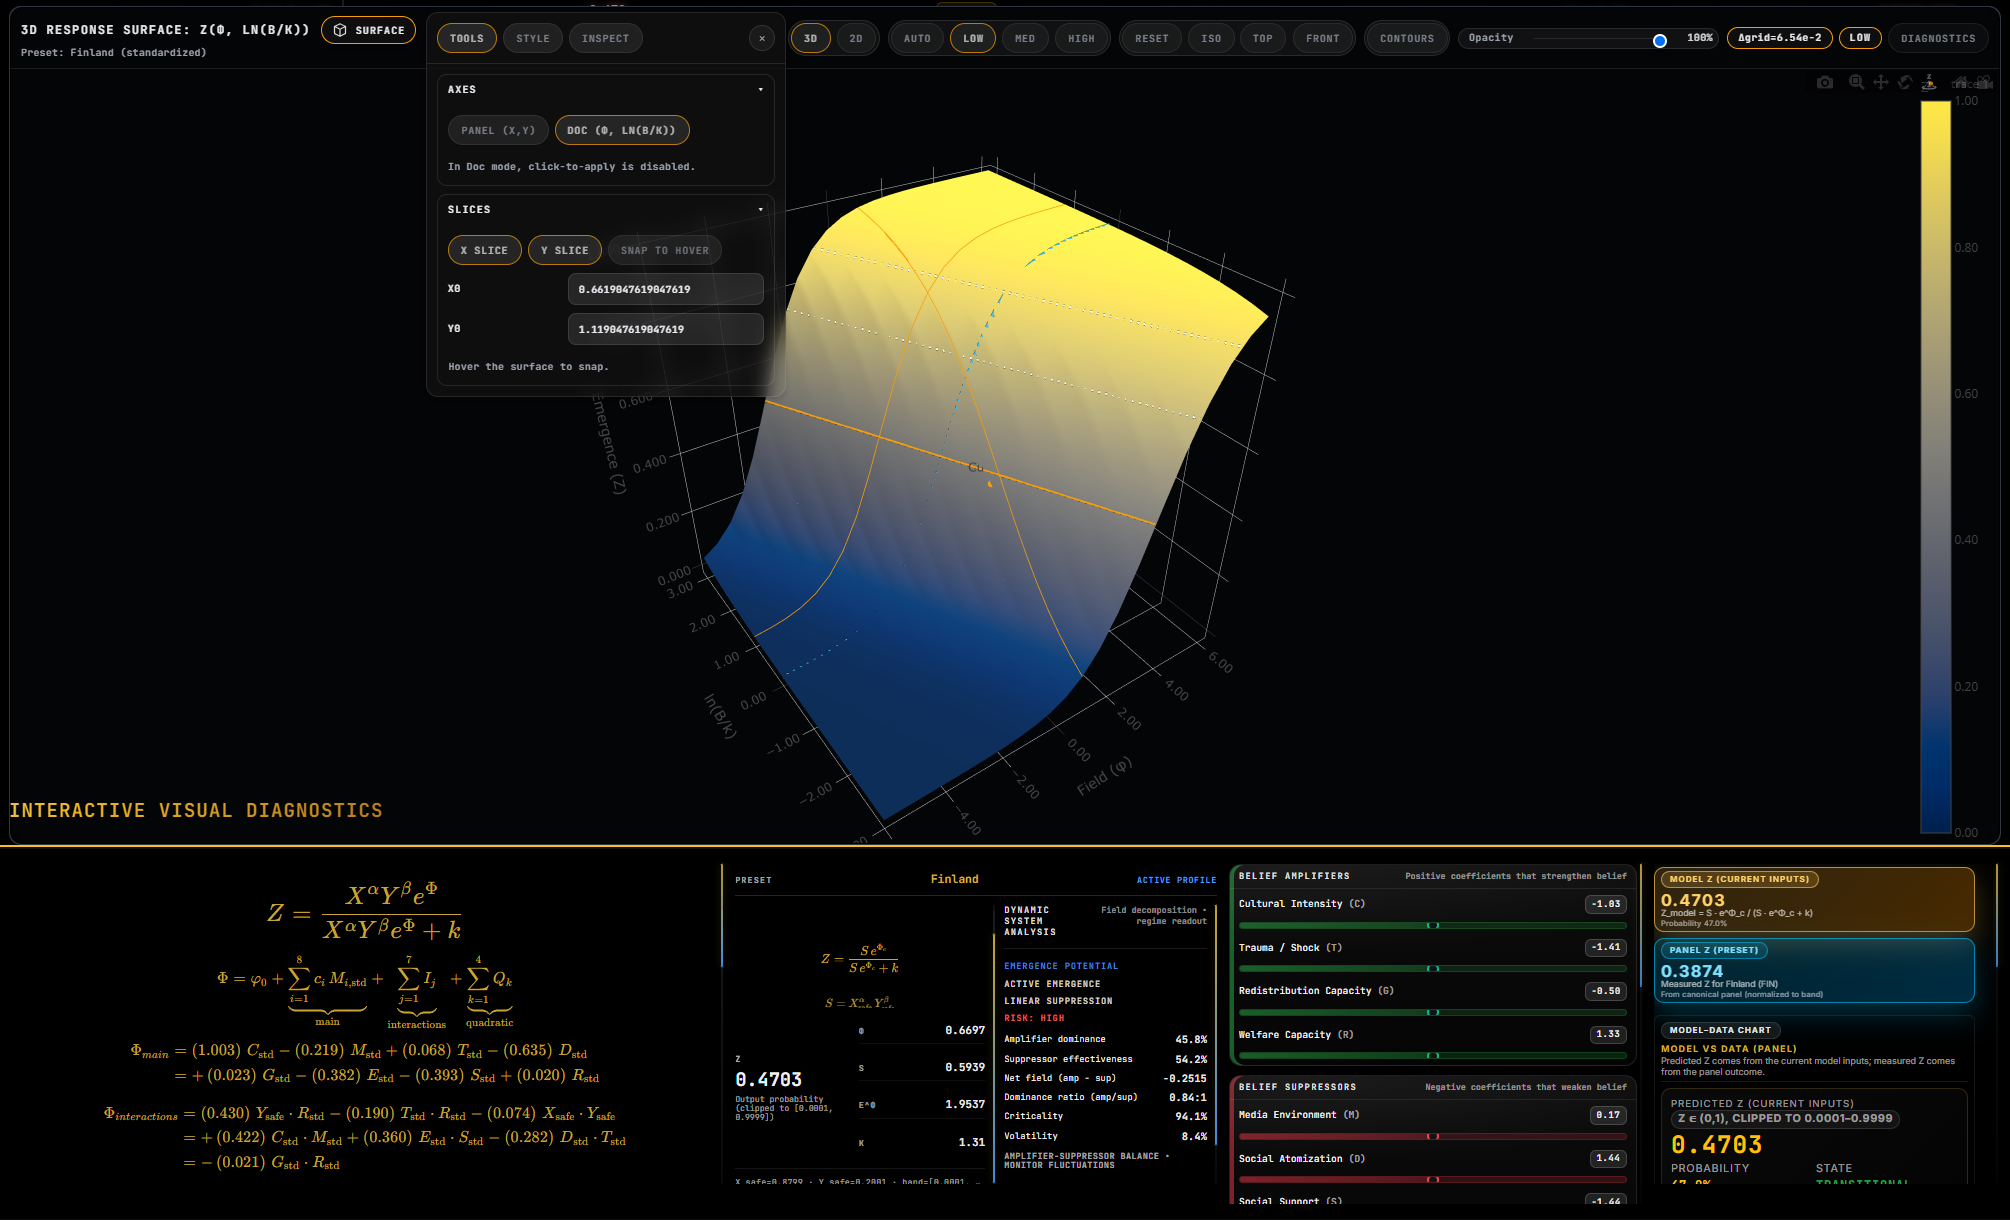
\includegraphics[width=\linewidth]{figure_A6_ui_screenshot_3.png}
    \caption{\textbf{Data scope:} supplementary UI screenshot showing a third interactive state snapshot. \textbf{Method context:} the capture documents how the UI presents model geometry and derived quantities for a specific deterministic parameter state. \textbf{Interpretation boundary:} this is an auditability record only, not a standalone inferential or causal figure.}
\end{figure}
\noindent\justifying
\textit{Reading note.} When comparing screenshots (3) and (4), the relevant scientific question is not whether the surface ``looks'' different, but whether the change corresponds to a controlled variation in the state vector.
The pinned-inspection mechanism is intended to enforce this control, so that qualitative differences can be traced to specific term-level contributions rather than implicit rescaling or navigation artifacts.
In practice, this means that any narrative comparison should be accompanied by an explicit statement of what was held fixed (preprocessing bounds, coefficients, and baseline $(X,Y)$) and what was changed (a specific modifier or preset), mirroring the finite-difference logic used in the regime-effect tables.
When this control is respected, screenshots can be treated as a compact experiment log for interpretability: they capture not only outcomes, but also the intermediate quantities that justify a mechanistic reading.
In practical review workflows, the most efficient use of these panels is to verify three items in sequence: (i) the state identity (preset name or pinned coordinates), (ii) the decomposition (which terms account for the net $\Phi$ shift), and (iii) the sensitivity (whether the local slope $\partial Z/\partial\Phi$ supports a meaningful change on the bounded scale).
If (i) and (ii) hold but (iii) indicates saturation, then changes in the surface may be visually salient but scientifically low-impact; conversely, when sensitivity is high, small compositional shifts can legitimately justify a large $\Delta Z$ narrative.
This discipline aligns the screenshot evidence with the finite-difference tables and prevents qualitative over-interpretation driven by display curvature alone.
\noindent\justifying
\textit{Operational guideline.} A useful way to treat each screenshot pair is as a two-condition sensitivity test: identify the single parameter or toggle that differs across states, and then ask whether the predicted change is aligned with the sign and regime pattern implied by the marginal-effect curves.
If a screenshot suggests a large qualitative shift but the corresponding finite-difference curve is flat in that regime, the most likely explanation is that the state lies on a low-sensitivity shoulder (bounded saturation) or that the two states are not truly comparable (hidden changes in preprocessing bounds or coefficients).
Conversely, when both the screenshot comparison and the curve agree (same sign, same high-sensitivity region), the interpretation is strengthened because two independent views of the same deterministic contract are consistent.
In practice, the most compact way to make this check auditable is to record the preset name or state hash in the export metadata and confirm it is identical across the two conditions.
\begin{figure}[!htbp]
    \centering
    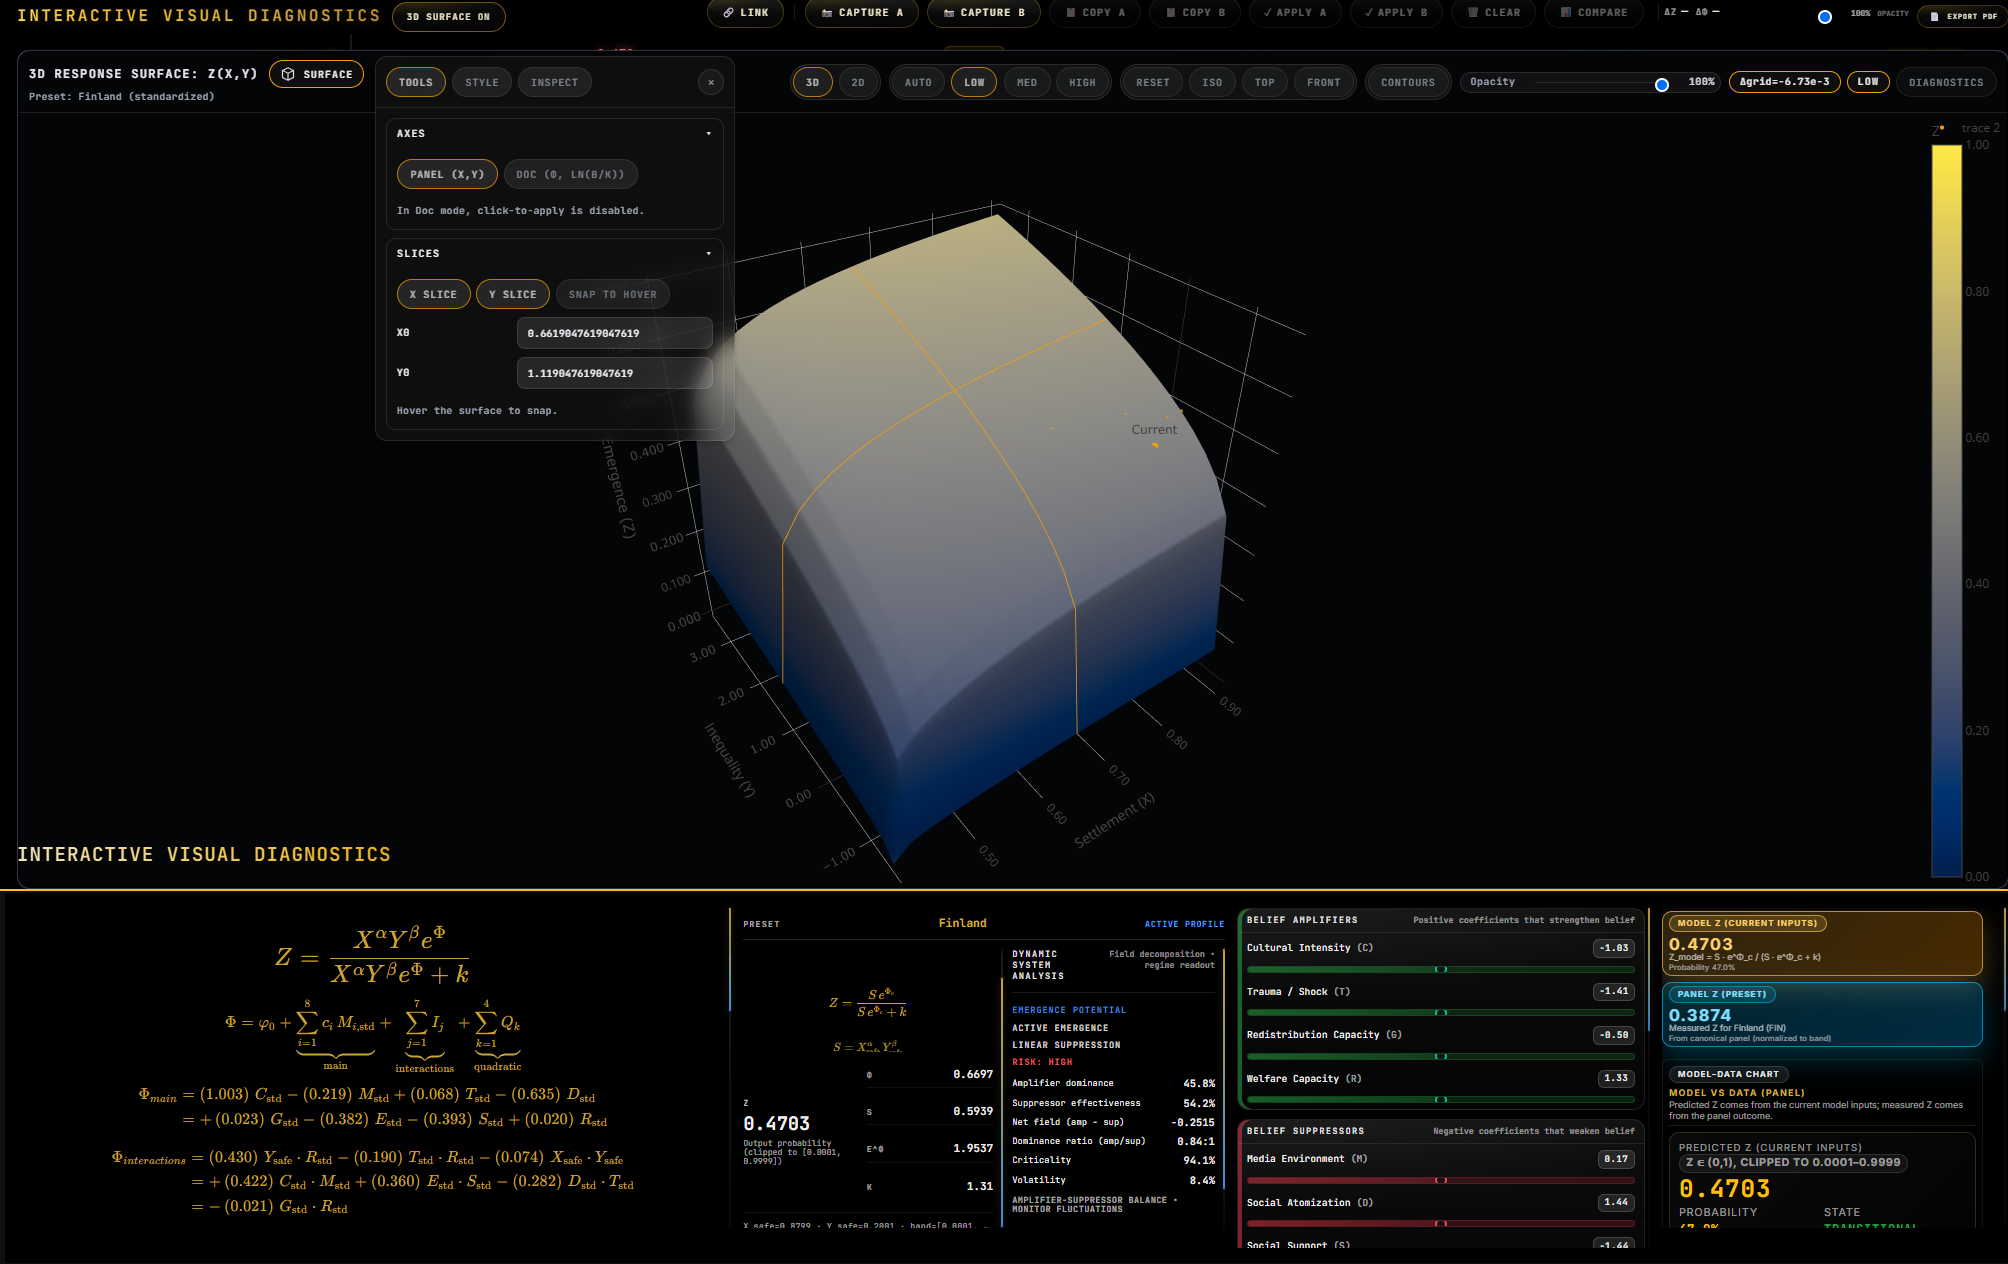
\includegraphics[width=\linewidth]{figure_A7_ui_screenshot_4.png}
    \caption{\textbf{Data scope:} supplementary UI screenshot showing an additional surface-instrument inspection state. \textbf{Method context:} the capture documents UI rendering under the bounded-transform safety logic and fixed coefficient artifacts during interactive exploration. \textbf{Interpretation boundary:} this is provenance documentation only; it does not introduce new inferential evidence.}
\end{figure}
\noindent\justifying
\textit{Curvature and sensitivity bands.} The UI overlay on the geometry surface shows predicted regions of high and low sensitivity, rendered as confidence or uncertainty bands around the central trajectory. These bands reflect the local slope and stability of the bounded transform near the current prediction level, making it visually clear where marginal effects are steep versus flat. Bright saturated regions indicate that small baseline perturbations produce large bounded responses, whereas pale or white regions indicate saturation or near-boundary behavior where the bounded map is less responsive.
\noindent\justifying
\textit{Why this matters for interpretation.} Because the mapping $Z=\sigma(\Phi+s)$ is bounded and non-linear, \emph{two} states can have very different decompositions while yielding similar $\widehat{Z}$ if both lie in a locally flat region.
For mechanistic narratives, the appropriate evidentiary standard is therefore twofold: (i) the decomposition must change in the hypothesized direction and (ii) the local sensitivity must be high enough that the bounded outcome can plausibly move.
The sensitivity overlays provide this second check directly at the point of inspection, reducing reliance on intuition about what a ``large'' visual change means.
\noindent\justifying
In the analysis workflow, these overlays serve as a guardrail: they prompt the analyst to prefer explanations rooted in the interior band (where $\partial Z/\partial\Phi$ is non-negligible) and to treat near-boundary visual variation as potentially cosmetic.
This is especially important when communicating amplifier/suppressor narratives, since term contributions to $\Phi$ can remain large even when the bounded response is locally insensitive.
\noindent\justifying
\textit{Interpretive guardrail.} When a surface appears visually dramatic, the question to ask is whether the state lies near the transition ridge (high sensitivity) or on a saturation shoulder (low sensitivity).
In the former case, moderate changes in $\Phi$ can legitimately imply a large bounded-scale movement; in the latter, similar changes should be interpreted as shifts in decomposition with limited outcome leverage.
The preset workflow below is designed to make this check routine by keeping the baseline state fixed and making any perturbation explicit.
\noindent\justifying
\textit{Reading note.} The preset mechanism below operationalizes this guardrail by packaging controlled starting points: the same named state can be reloaded, pinned, and exported so that any downstream figure is tied to an identical parameterization.
This makes regime comparisons reproducible and limits post-hoc reinterpretation driven by accidental navigation to a different sensitivity region.
As a consequence, disagreements between two narrative readings can be adjudicated by reloading the same preset and checking whether (i) the decomposition changes as claimed and (ii) the local sensitivity supports the claimed bounded-scale impact.
\begin{figure}[!htbp]
    \centering
    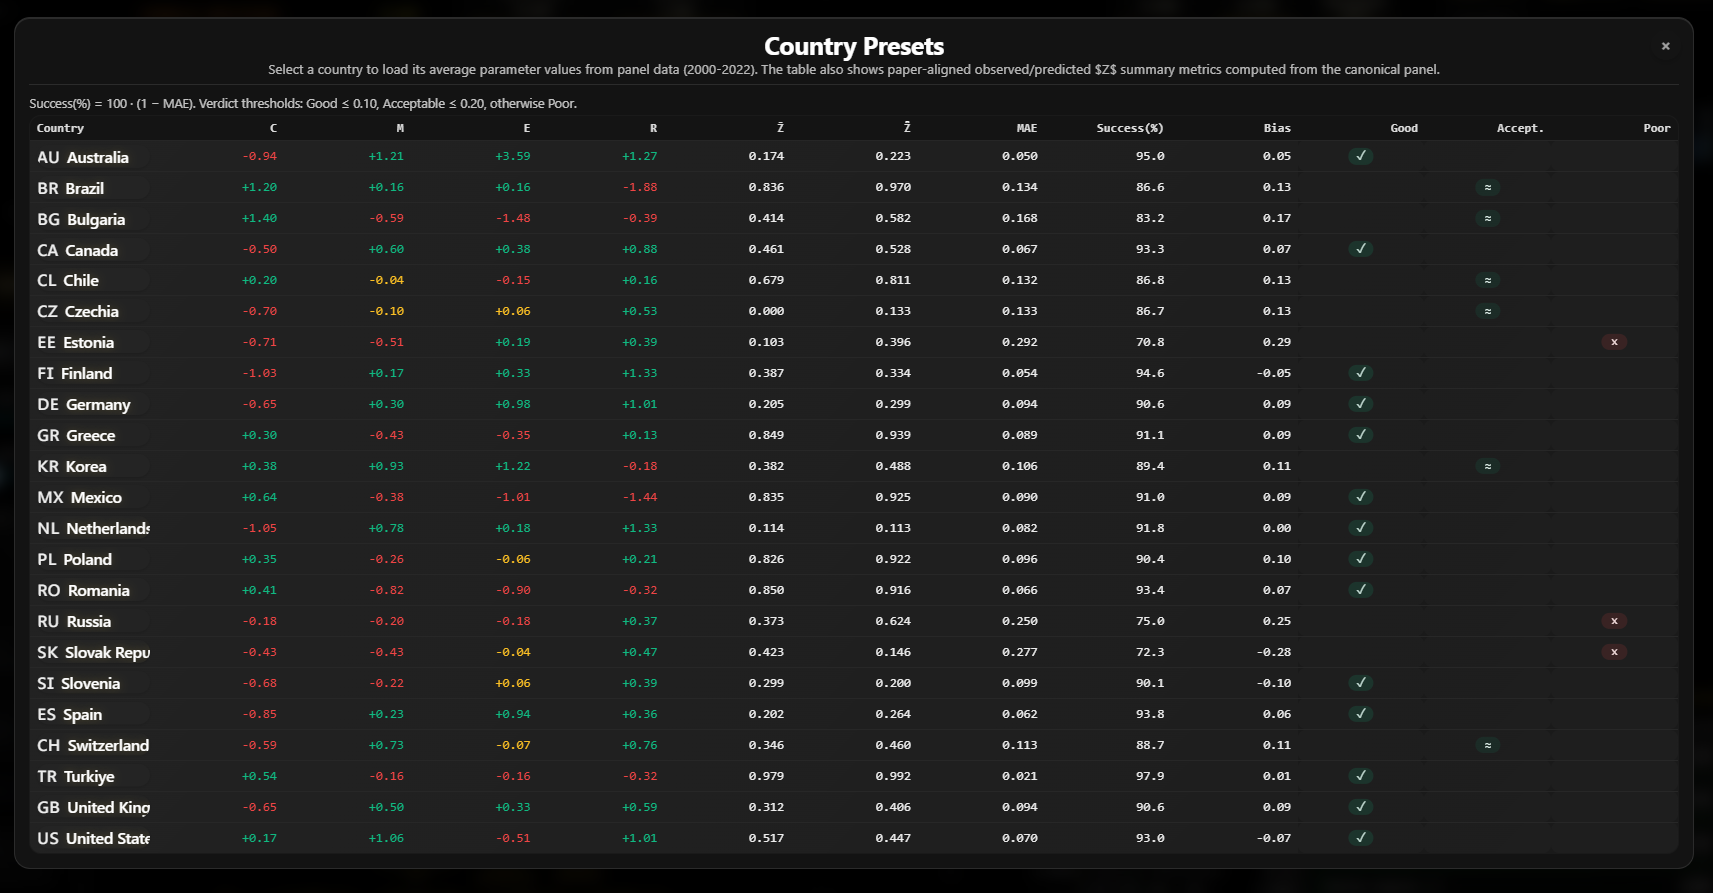
\includegraphics[width=\linewidth]{figure_9_ui_presets.png}
    \caption{\textbf{Data scope:} supplementary preset-configuration views for reproducible UI state vectors. \textbf{Method context:} the views document how named preset bundles synchronize sliders and toggles before comparing $\Phi$ decomposition and the resulting bounded response surface $Z$. \textbf{Interpretation boundary:} this is a provenance/control-mechanism figure only, not inferential evidence.}
\end{figure}
\noindent\justifying
\textit{Preset mechanism and reproducibility.} Presets encode fixed parameter bundles as named snapshots within the interactive state vector. When a preset is activated, all sliders, toggles, and diagnostic view settings are synchronized to the preset's stored configuration, ensuring that comparisons across two or more states reflect only the intended variation. The preset labels (e.g., ``baseline regime,'' ``high urbanization scenario'') are user-defined and serve as mnemonics for interpretable scenario labels; the underlying numerical values are deterministically exported alongside the figure, guaranteeing external reproducibility.
\begin{figure}[!htbp]
    \centering
    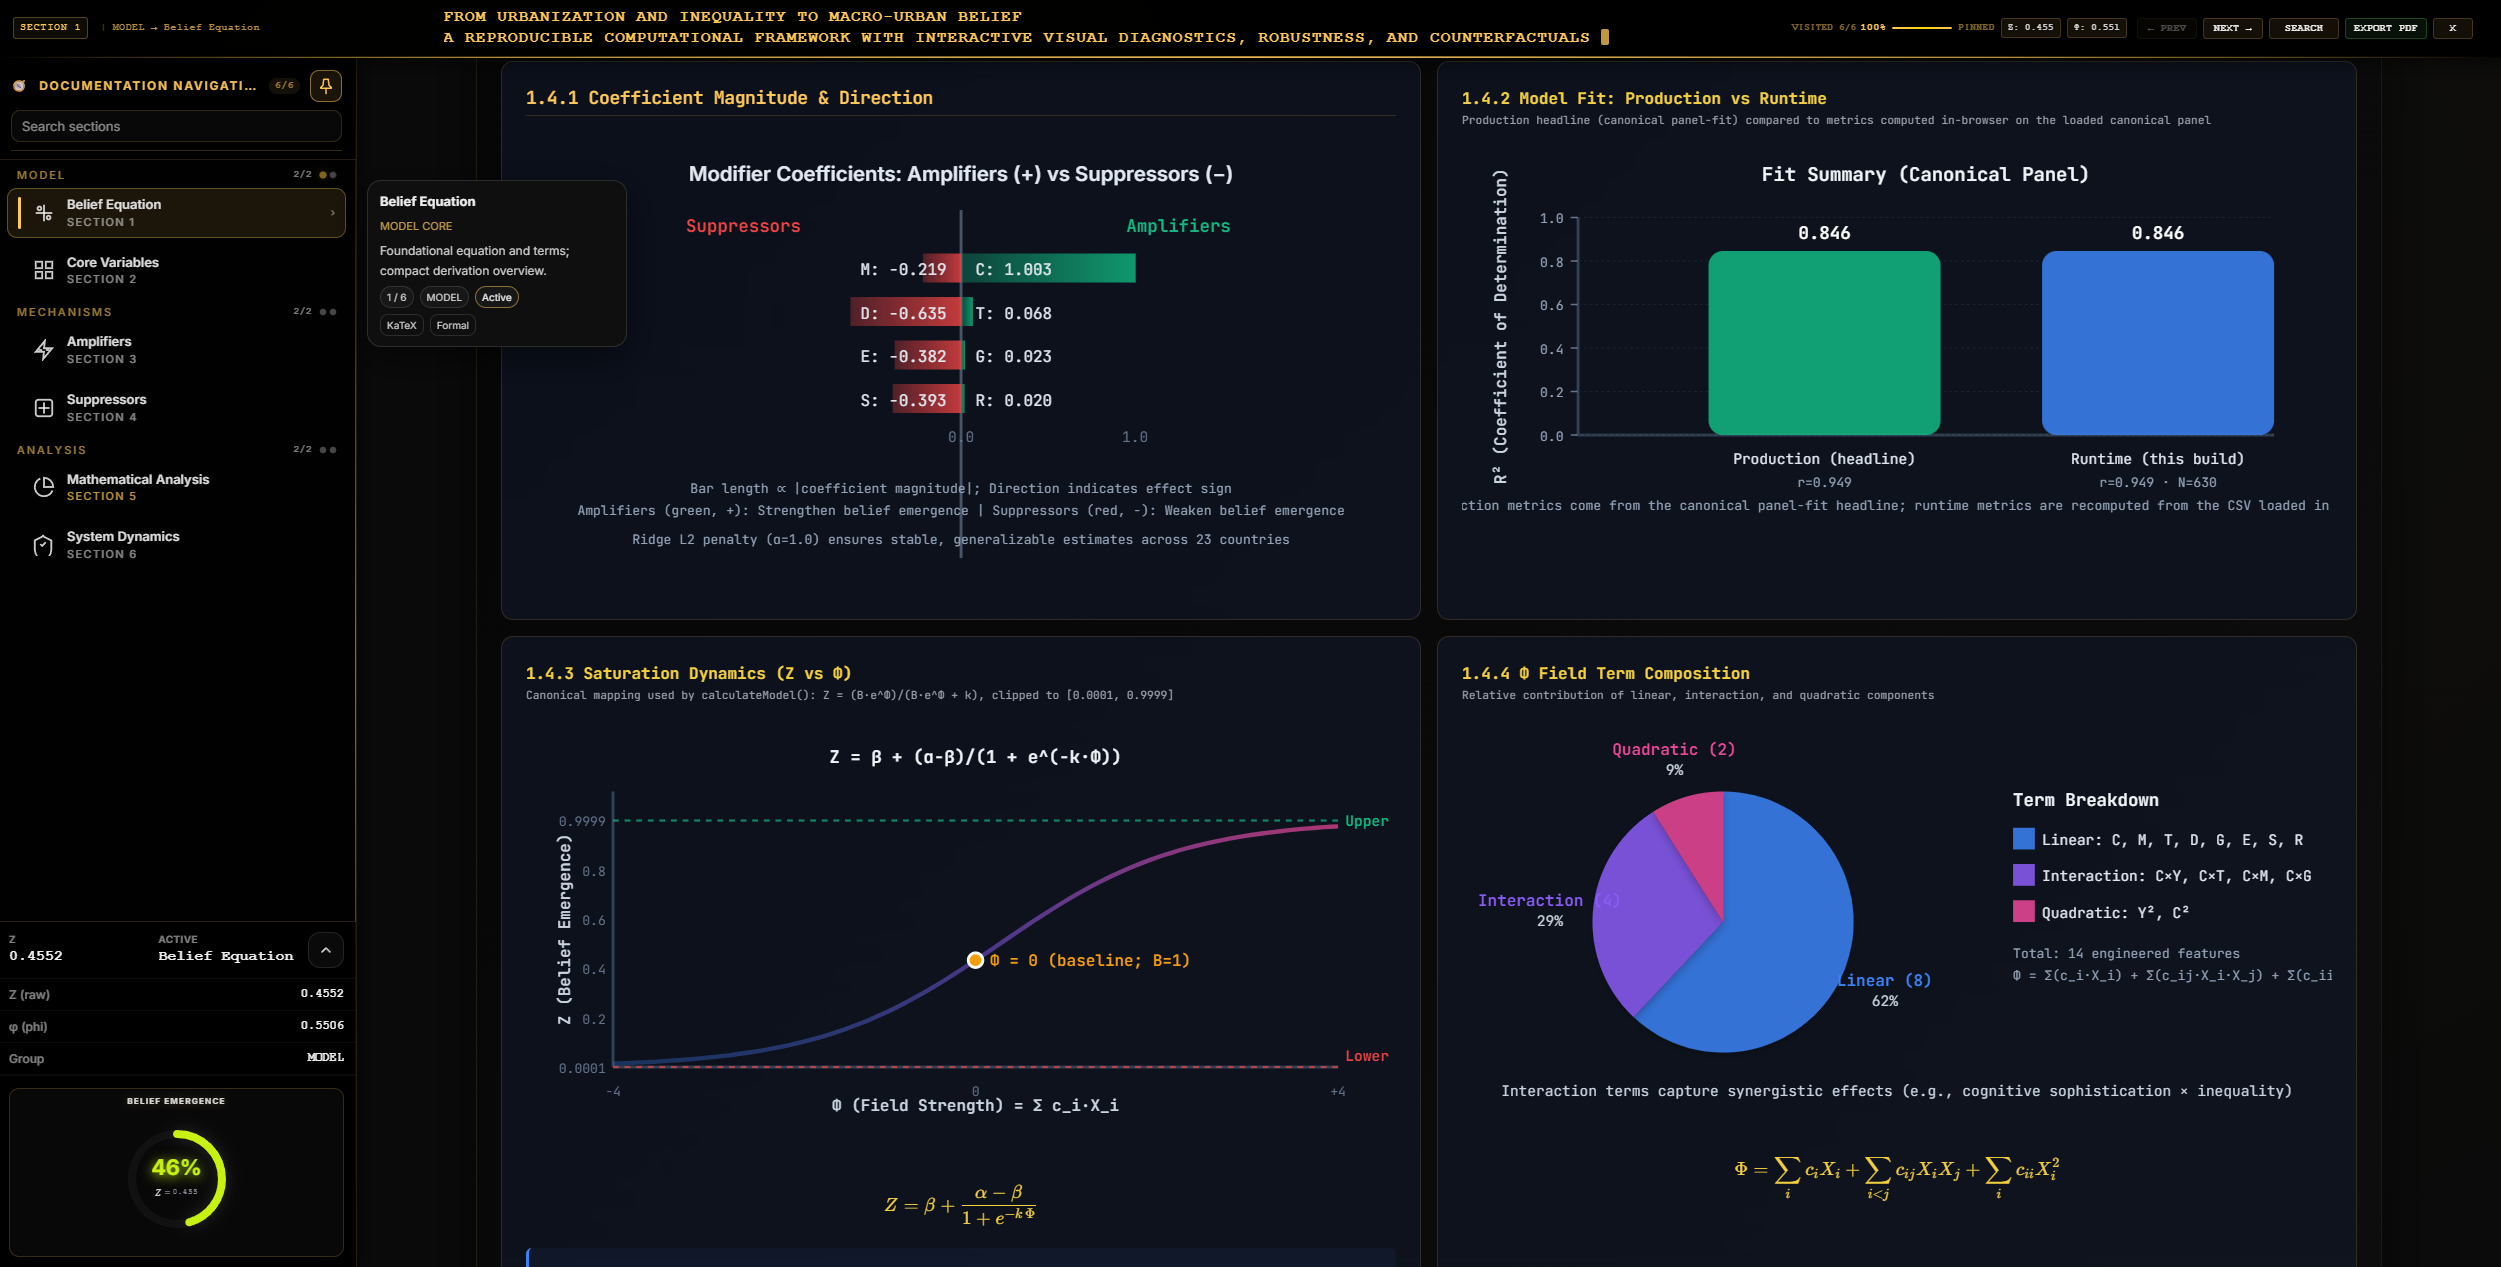
\includegraphics[width=\linewidth]{figure_A9_belief_equation_panel.png}
    \caption{\textbf{Data scope:} screenshot of the belief-equation display panel. \textbf{Method context:} the UI renders the computational form of the belief field $\Phi$ and the bounded transform as an inspectable object linking interactive parameters to additive components and the downstream response $Z$. \textbf{Interpretation boundary:} this is interpretability-layer documentation only, not independent evidence or causal support.}
\end{figure}
\begin{figure}[!htbp]
    \centering
    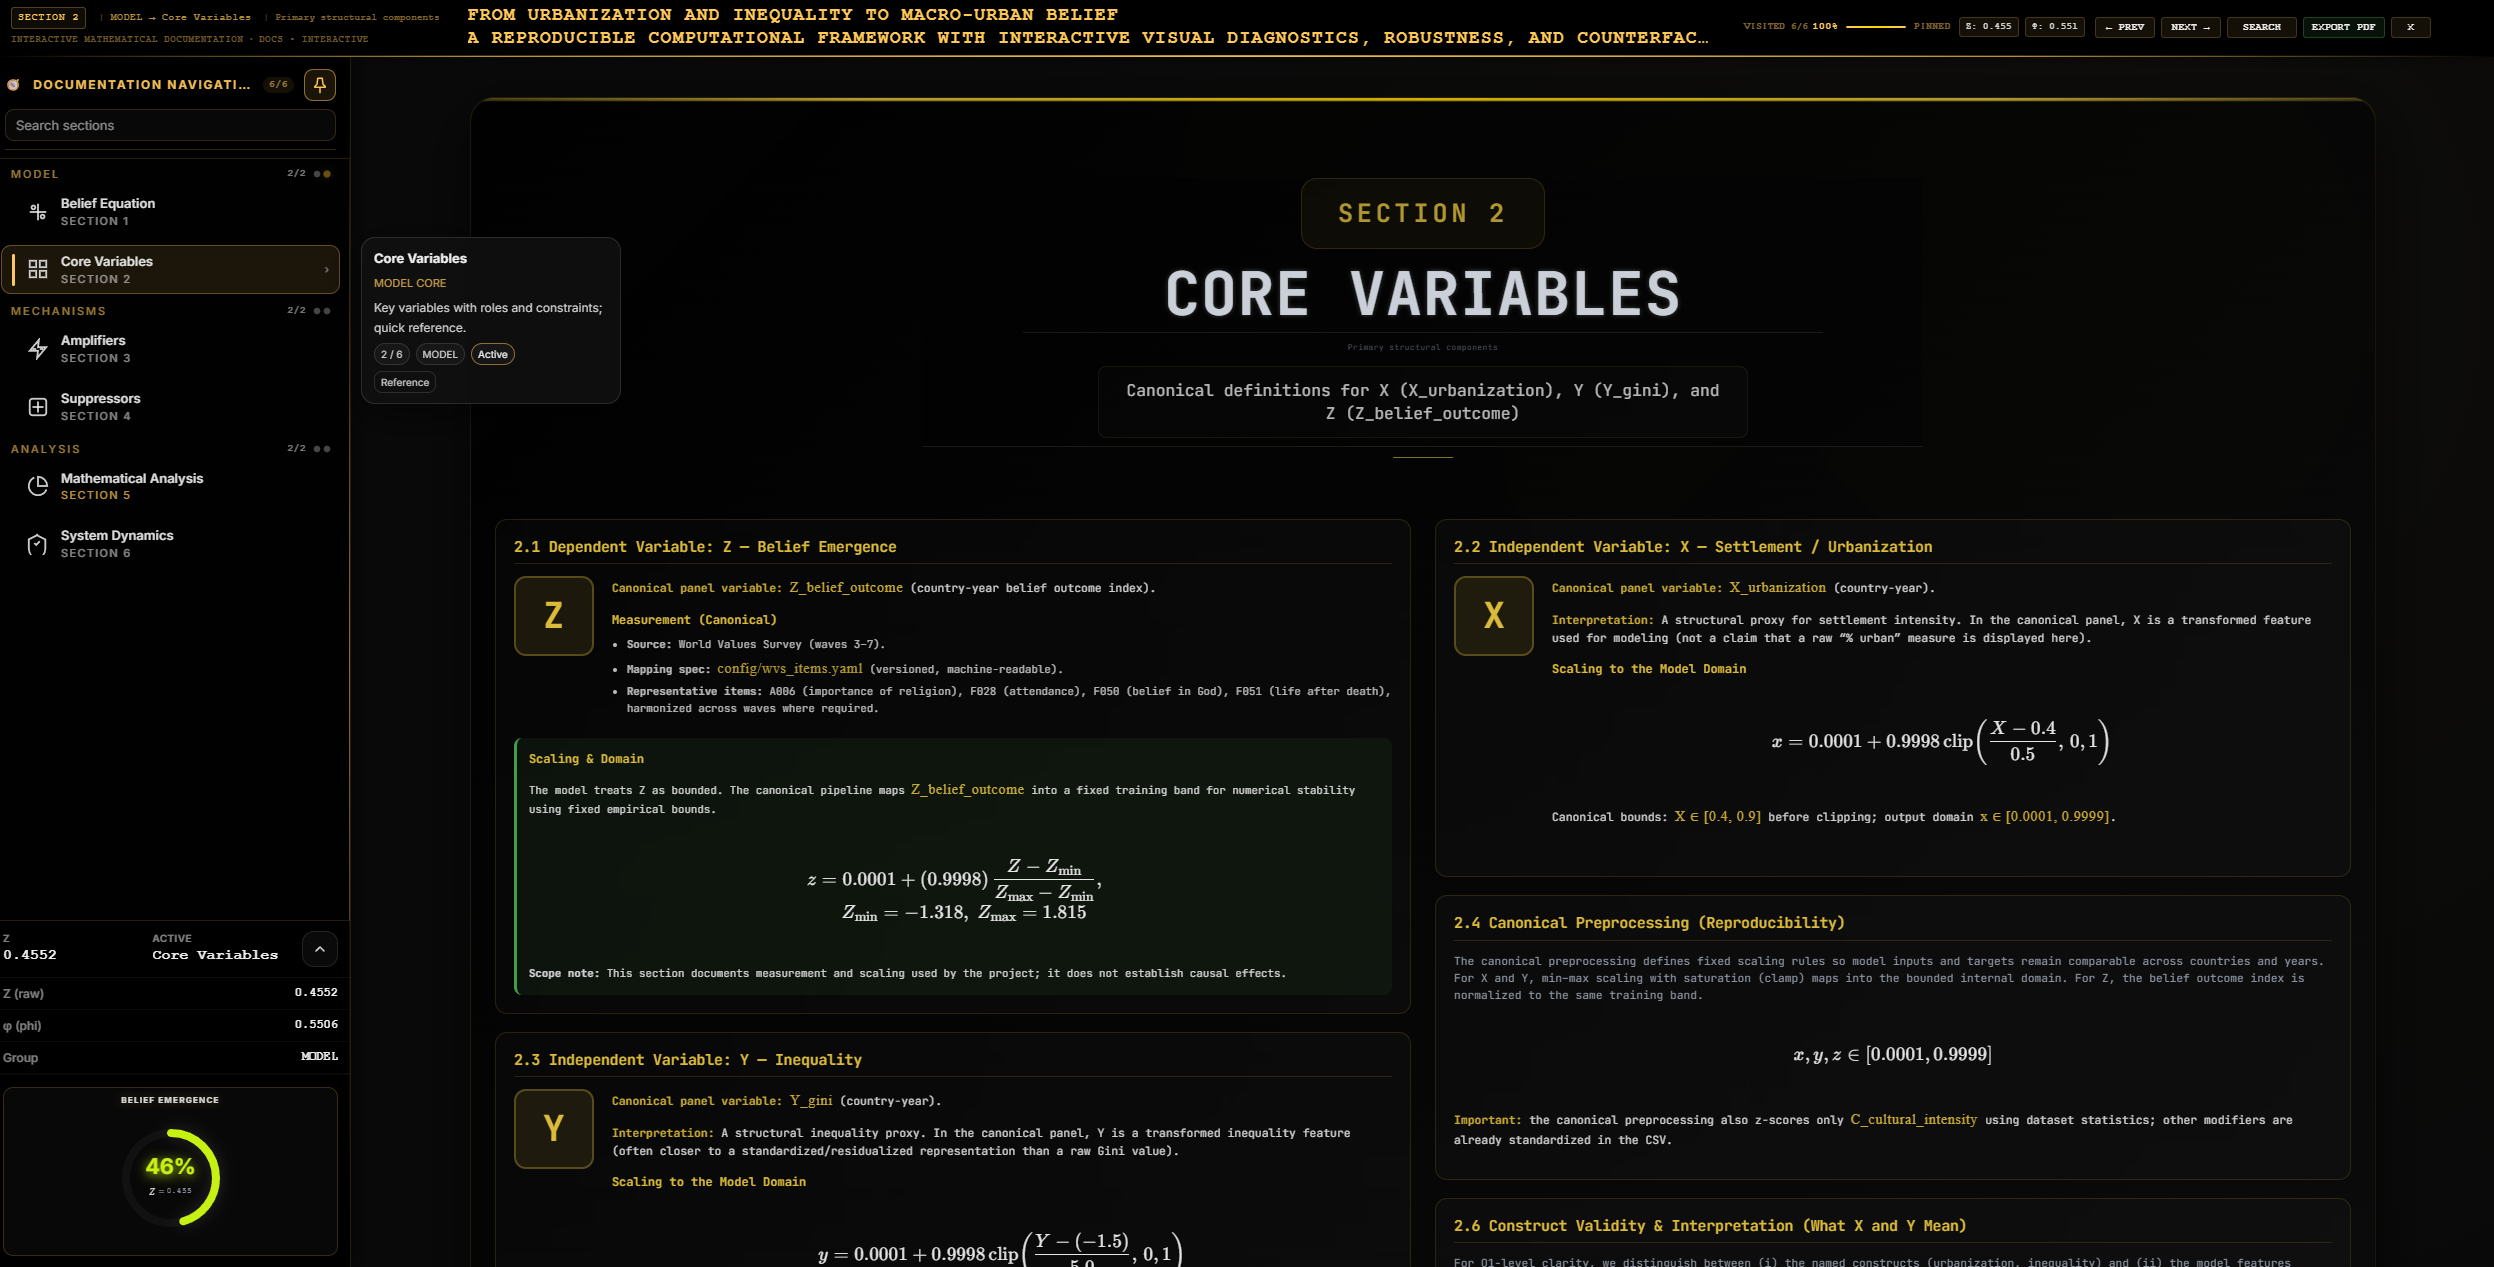
\includegraphics[width=\linewidth]{figure_A10_core_variables_panel.png}
    \caption{\textbf{Data scope:} screenshot of the core-variable control panel. \textbf{Method context:} the panel documents the standardized controls exposed for interactive exploration of the $(X,Y)$ stimulus terms under fixed preprocessing bounds. \textbf{Interpretation boundary:} this is UI provenance only; it is not inferential evidence.}
\end{figure}
\begin{figure}[!htbp]
    \centering
    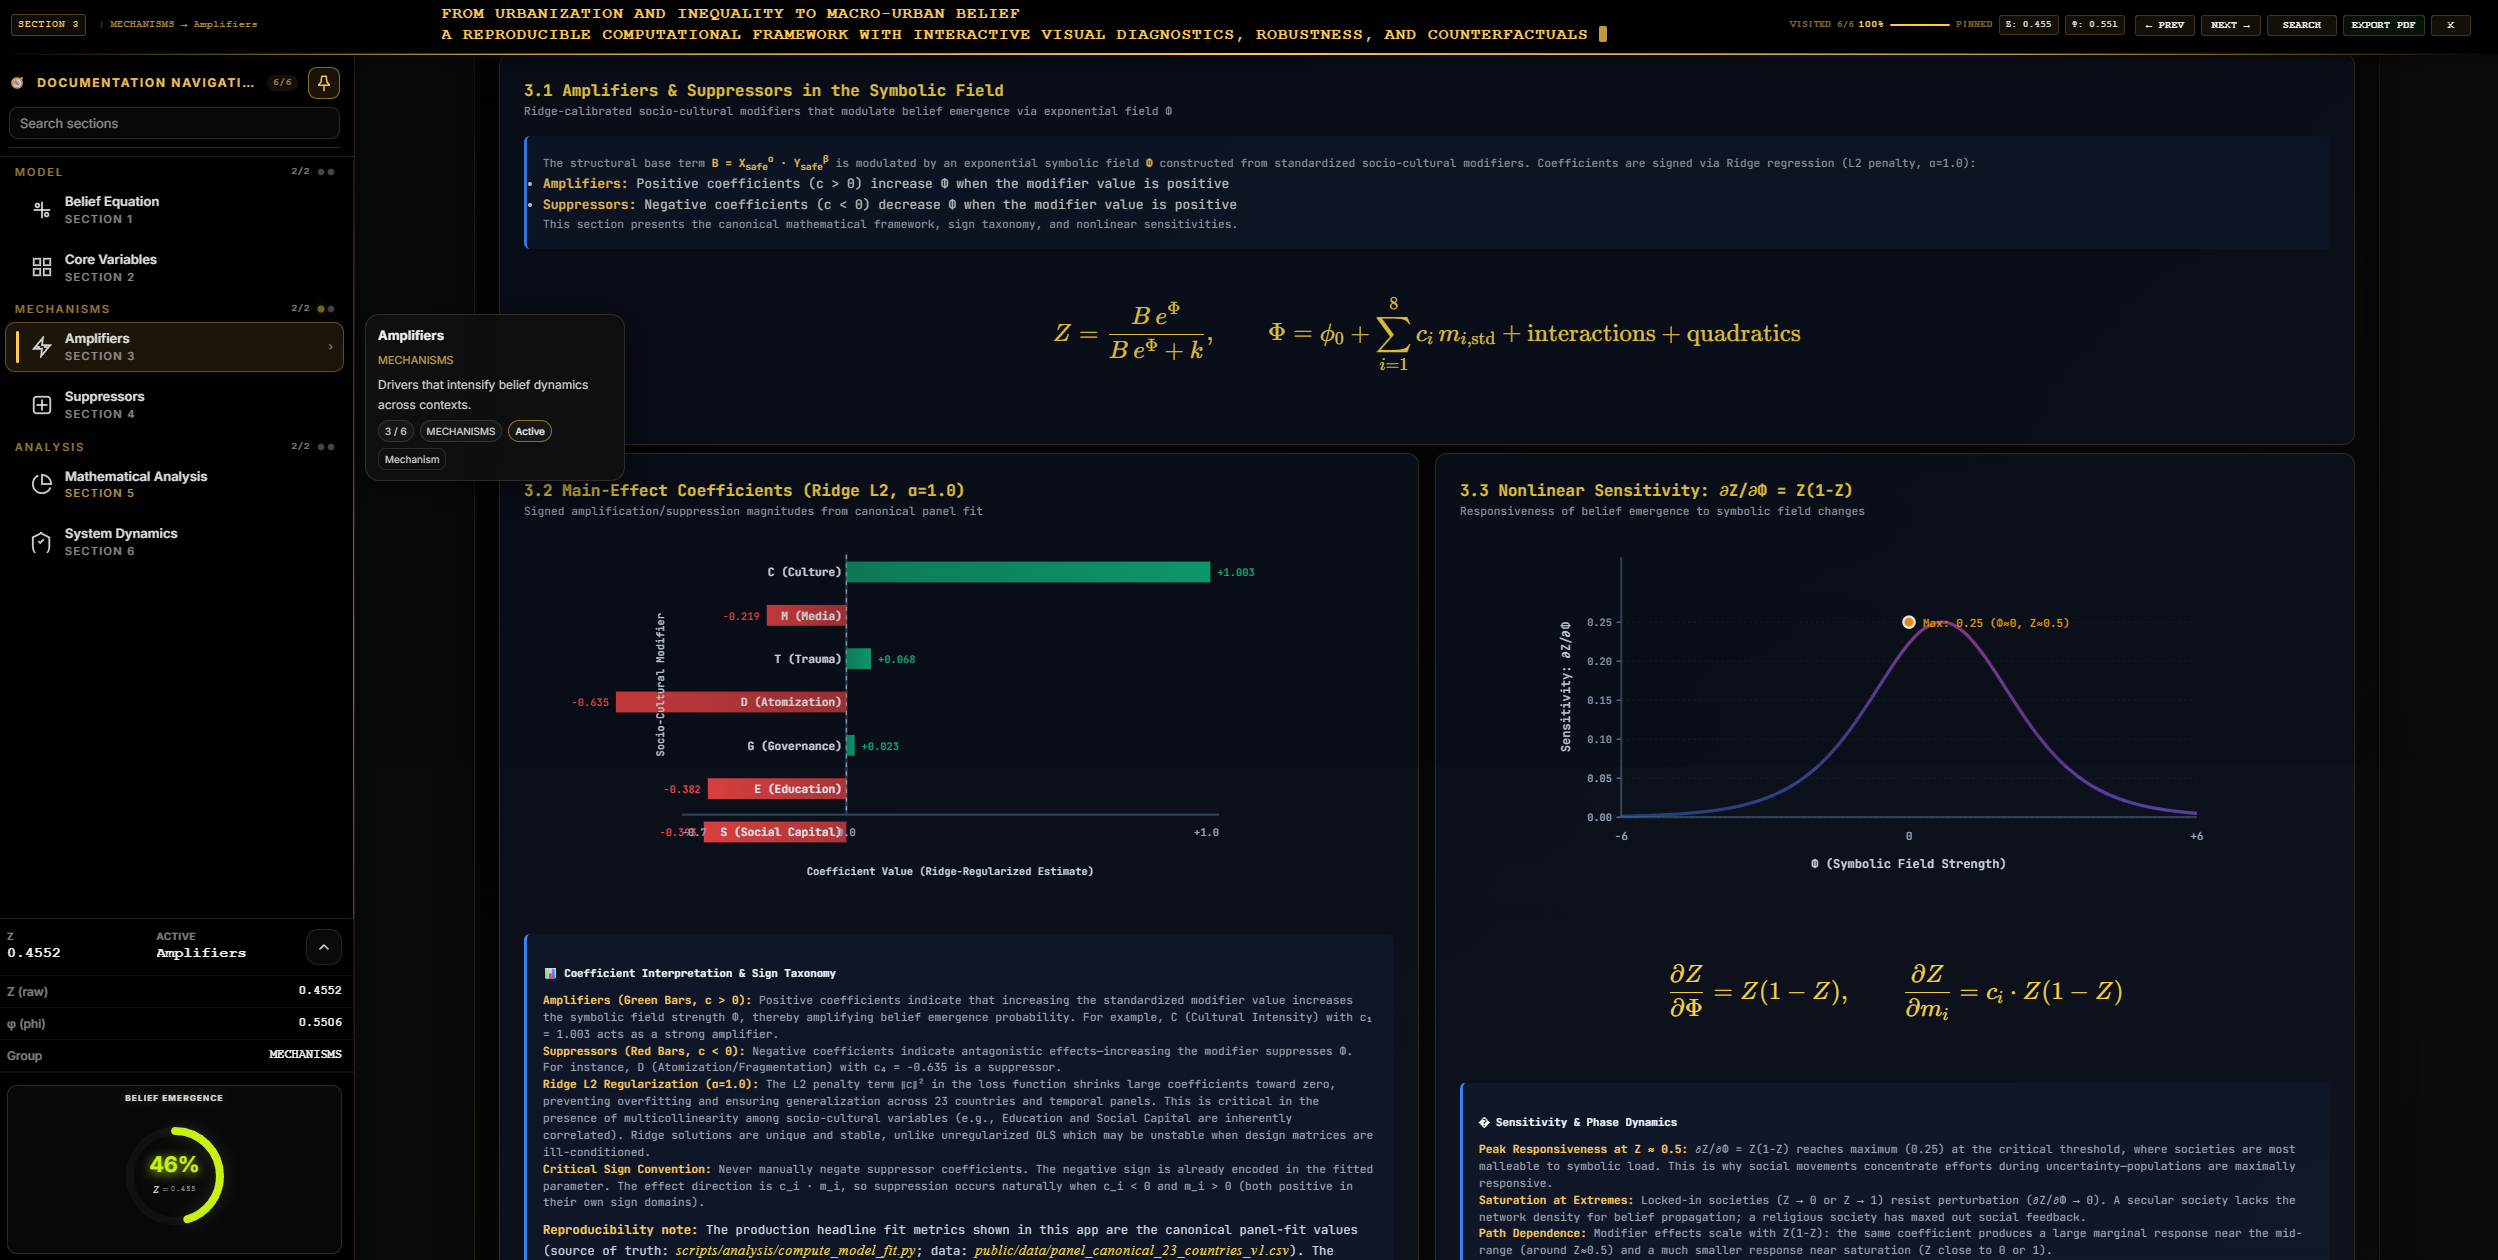
\includegraphics[width=\linewidth]{figure_A11_amplifiers_panel.png}
    \caption{\textbf{Data scope:} screenshot of the belief-amplifier panel. \textbf{Method context:} the UI decomposes $\Phi$ into signed additive components and surfaces positive state-specific contributions under the current deterministic state vector. \textbf{Interpretation boundary:} this is a local interpretability aid only; it is not global sign evidence, Tier A/B validation, or causal proof.}
\end{figure}
\noindent\justifying
\textit{Reading note.} The amplifier and suppressor panels should be interpreted as paired views of the same additive decomposition: a term can move between panels across regimes as the state changes, even when its global coefficient sign is fixed.
This is expected in interaction-rich specifications, and it is precisely why state-anchored, deterministic inspection is emphasized rather than universal sign narratives.
\begin{figure}[!htbp]
    \centering
    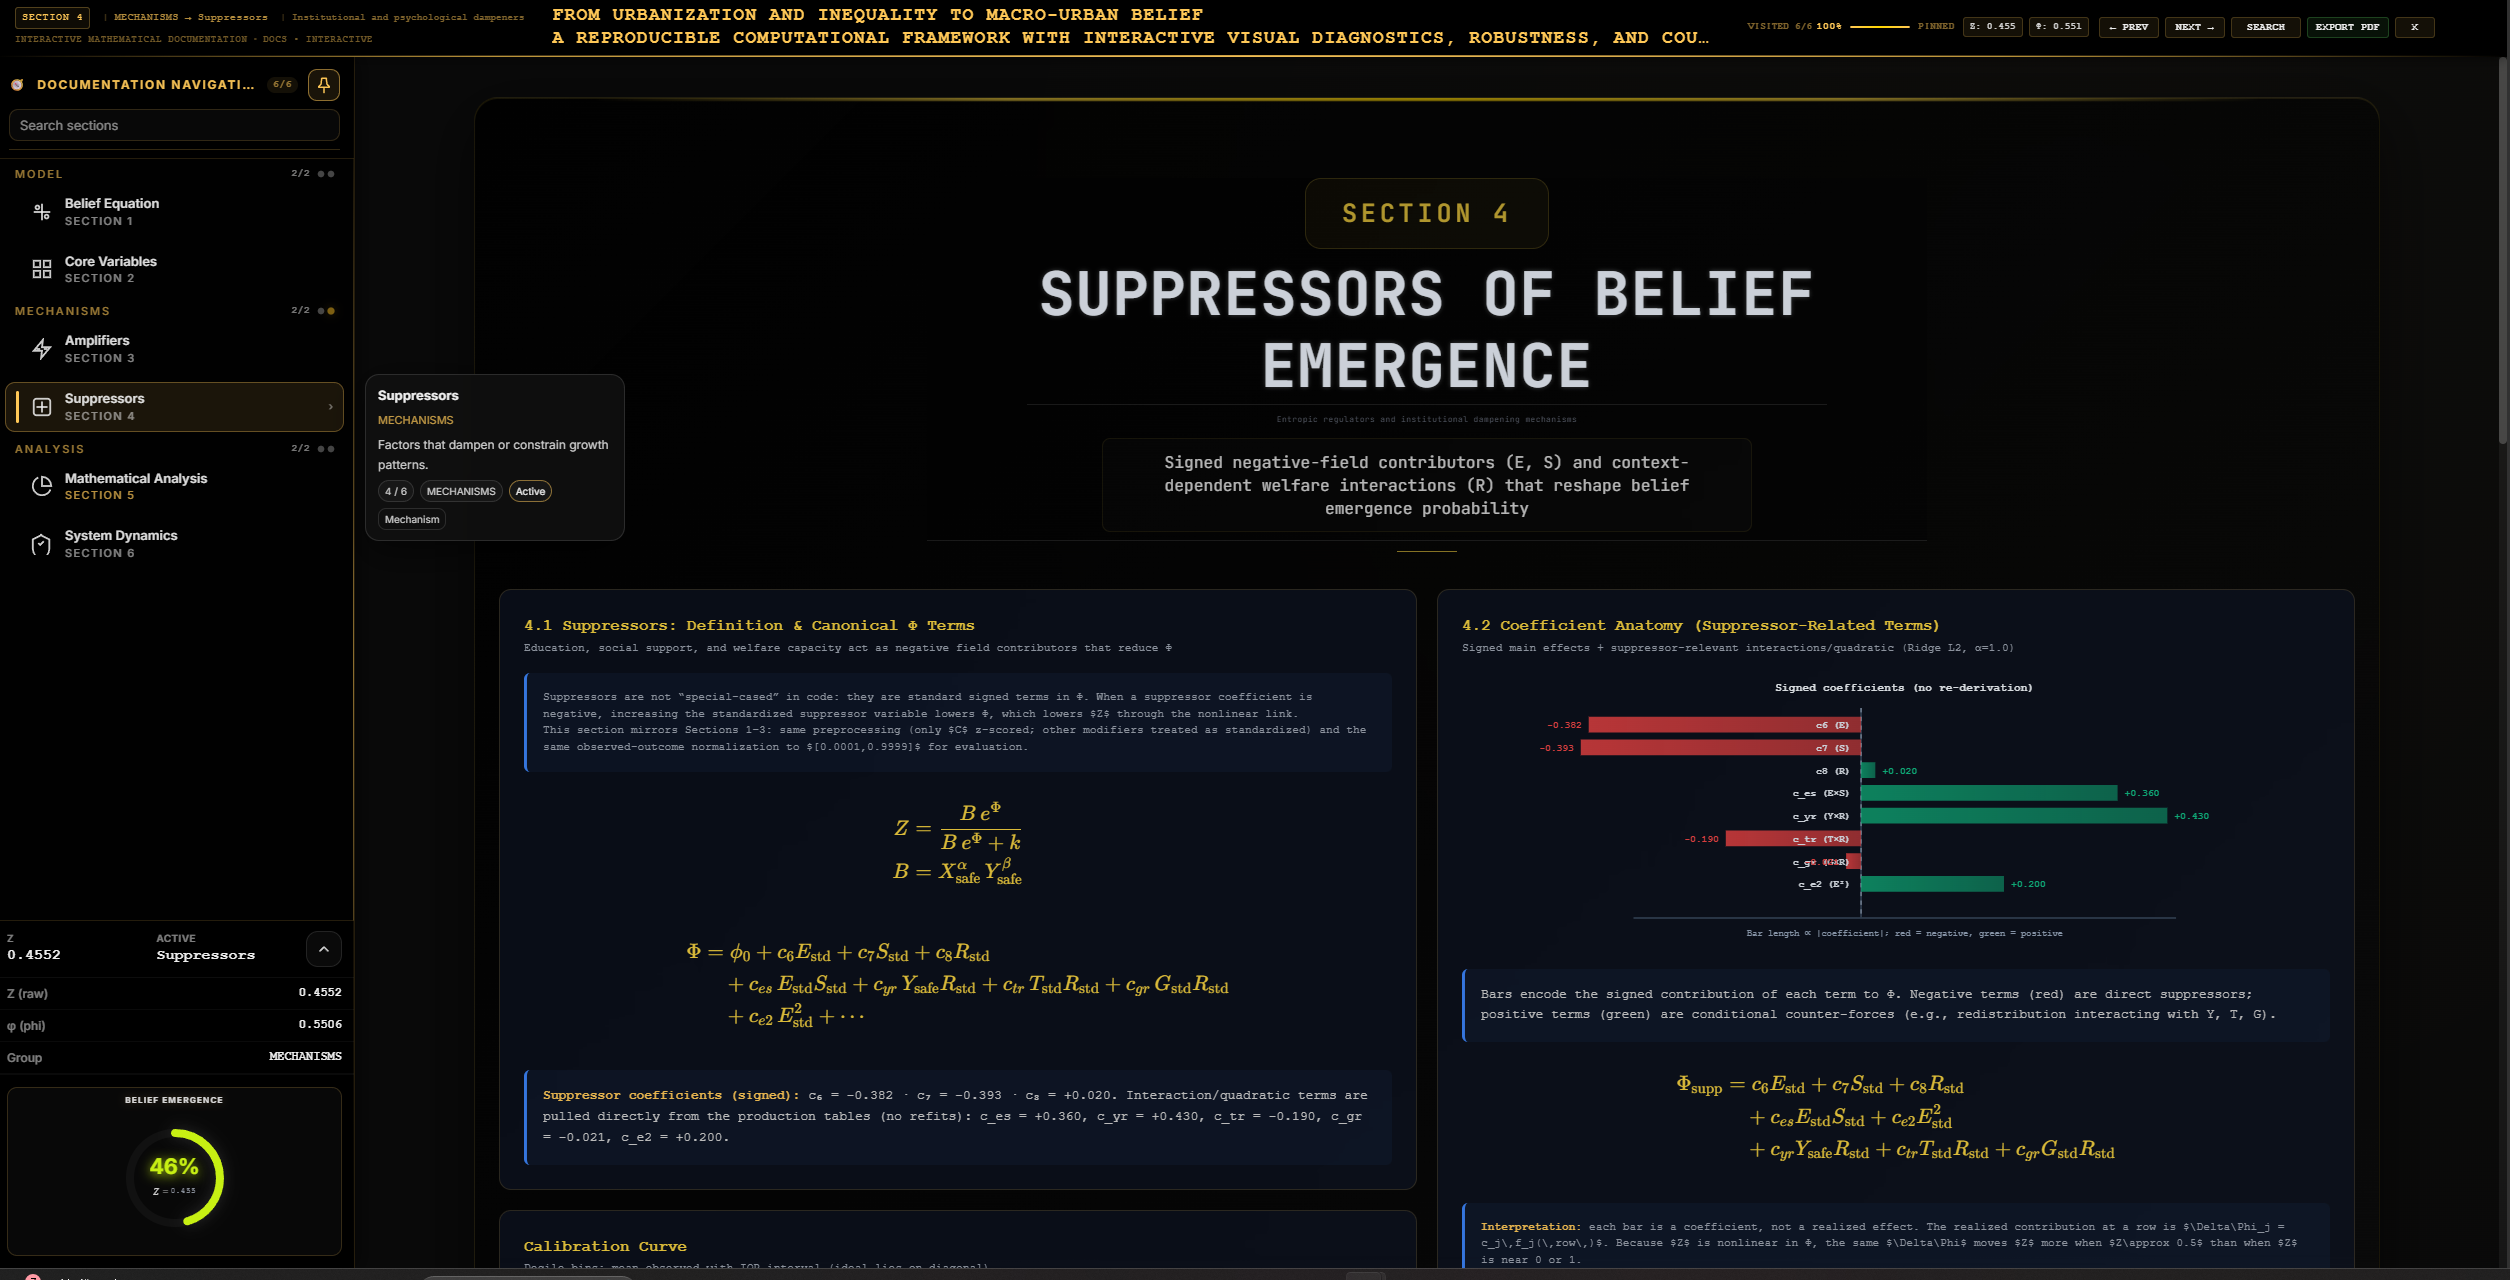
\includegraphics[width=\linewidth]{figure_A12_suppressors_panel.png}
    \caption{\textbf{Data scope:} screenshot of the belief-suppressor panel. \textbf{Method context:} complementary to the amplifier view, the panel enumerates negative state-specific contributions to $\Phi$ under the current deterministic state. \textbf{Interpretation boundary:} this is a local interpretability aid only; it is not global sign evidence or causal proof.}
\end{figure}
\begin{figure}[!htbp]
    \centering
    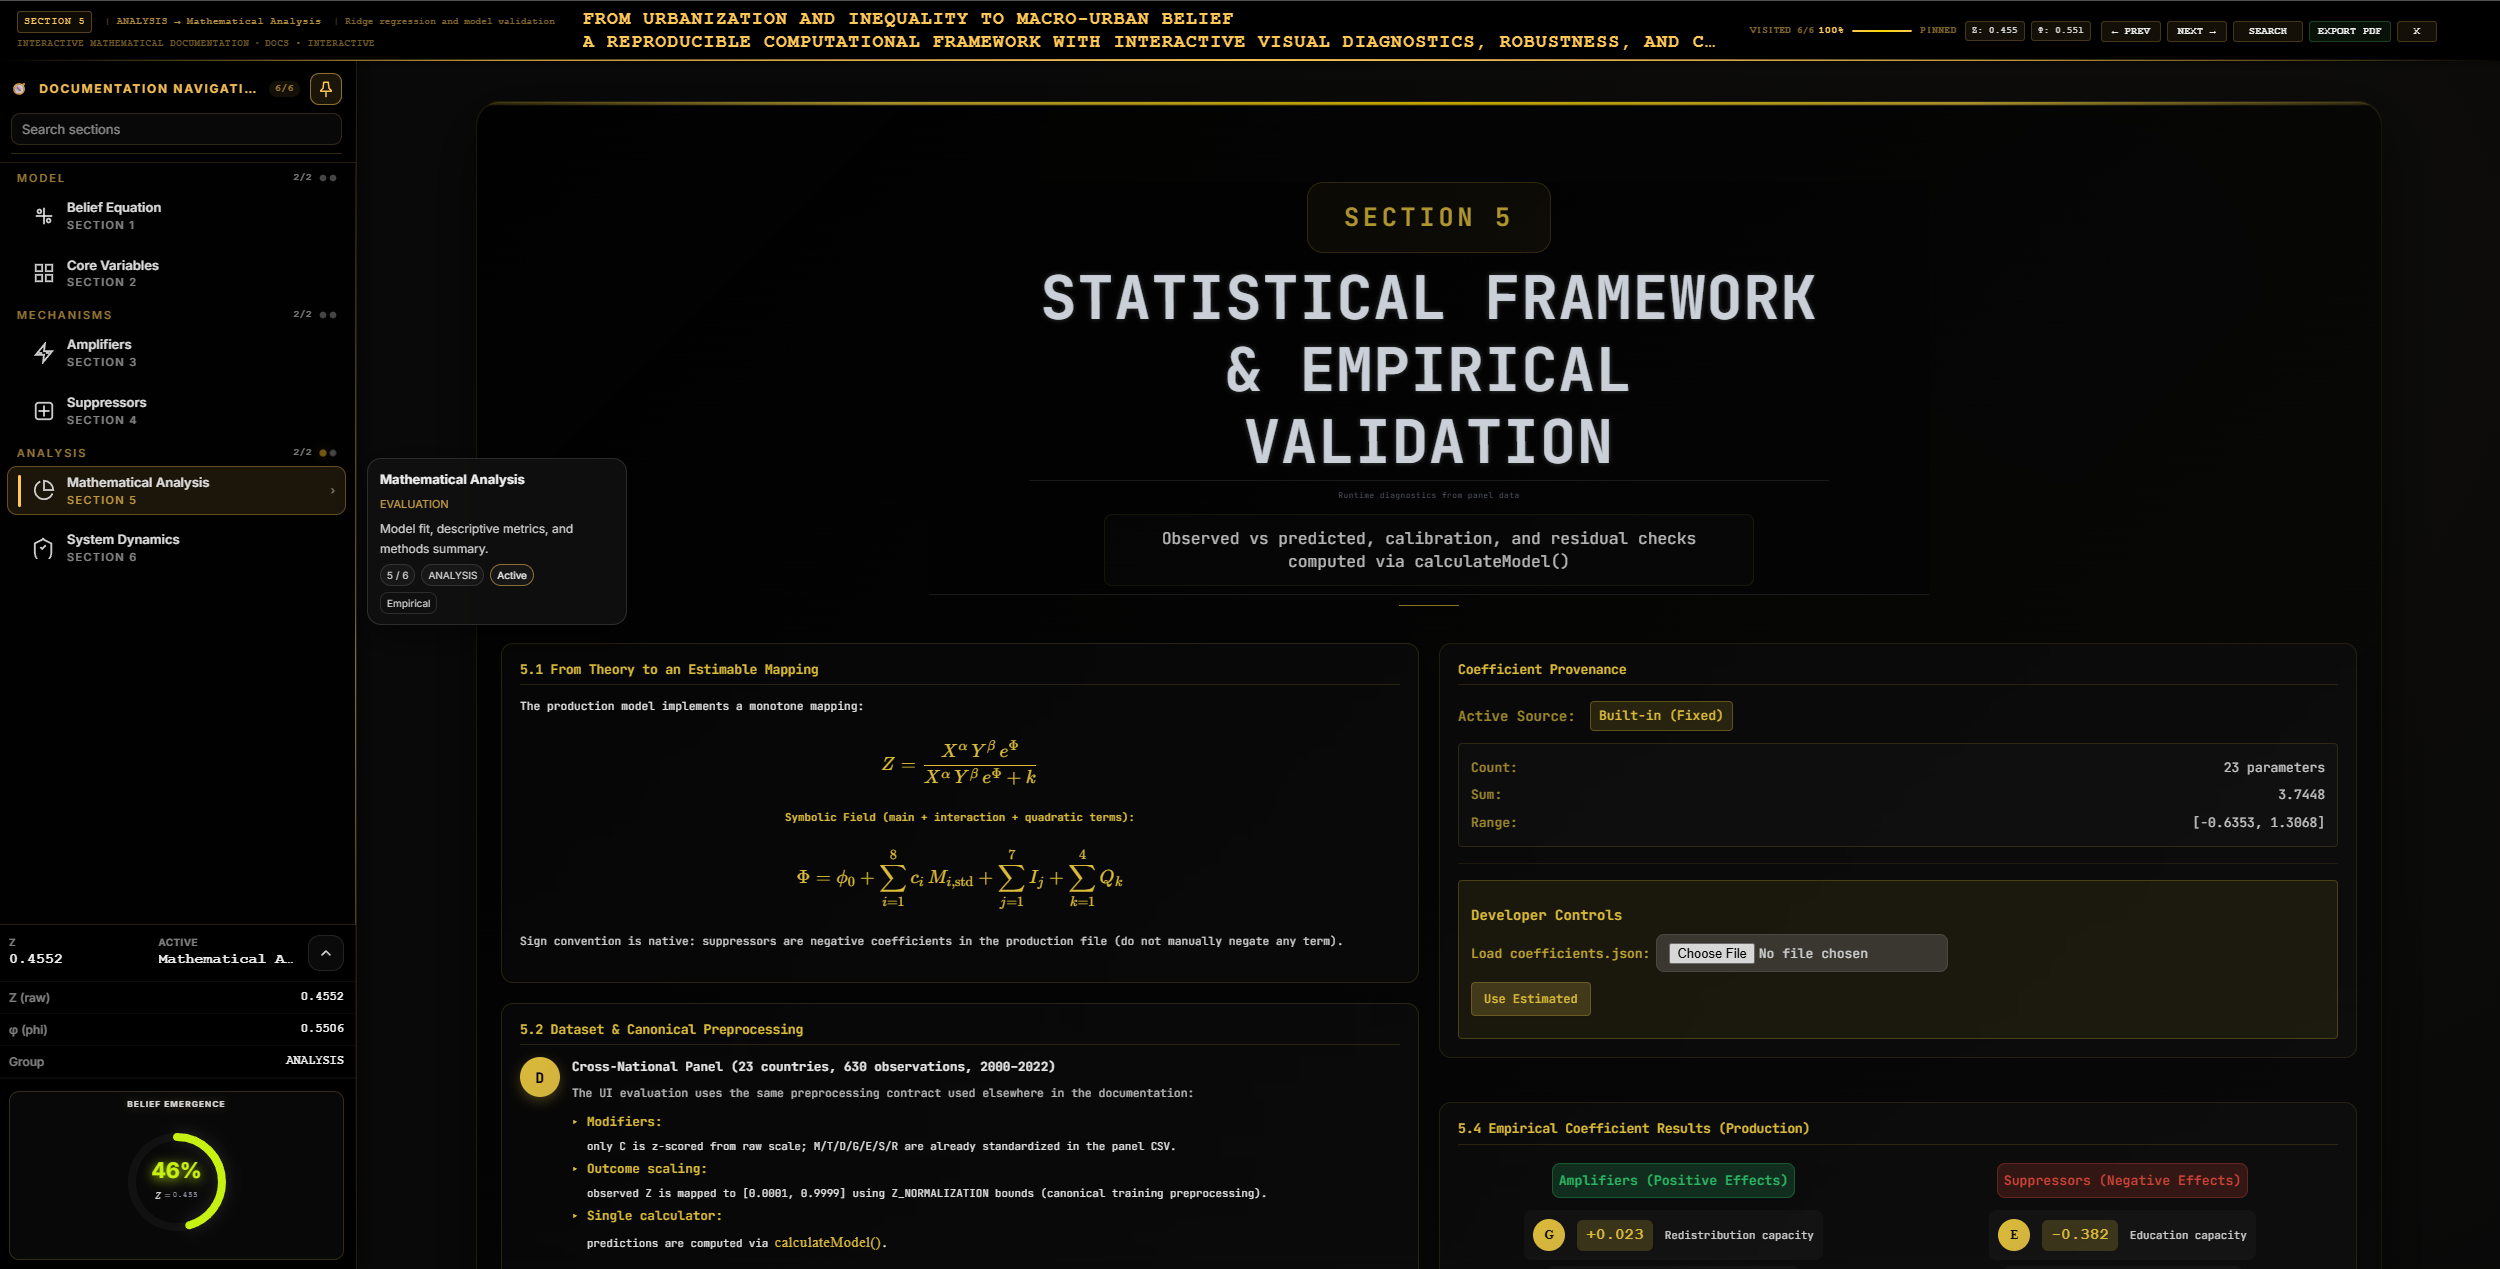
\includegraphics[width=\linewidth]{figure_A13_mathematical_analysis_panel.png}
    \caption{\textbf{Data scope:} screenshot of the mathematical-analysis diagnostics panel. \textbf{Method context:} the panel aggregates residual, calibration-style, and slice-summary checks available in the UI under the fixed-coefficient contract. \textbf{Interpretation boundary:} this is a convenience provenance panel only; primary evidence remains the manuscript evaluation figures and tables.}
\end{figure}
\noindent\justifying
\textit{Reading note.} This diagnostics panel is intended as a convenience aggregation: it helps verify that a pinned state sits in a region with adequate support and that local explanatory narratives are not contradicted by gross residual structure.
In other words, it supports sanity checks during exploration, while the primary evidence remains the manuscript-consistent evaluation figures and tables.
\begin{figure}[!htbp]
    \centering
    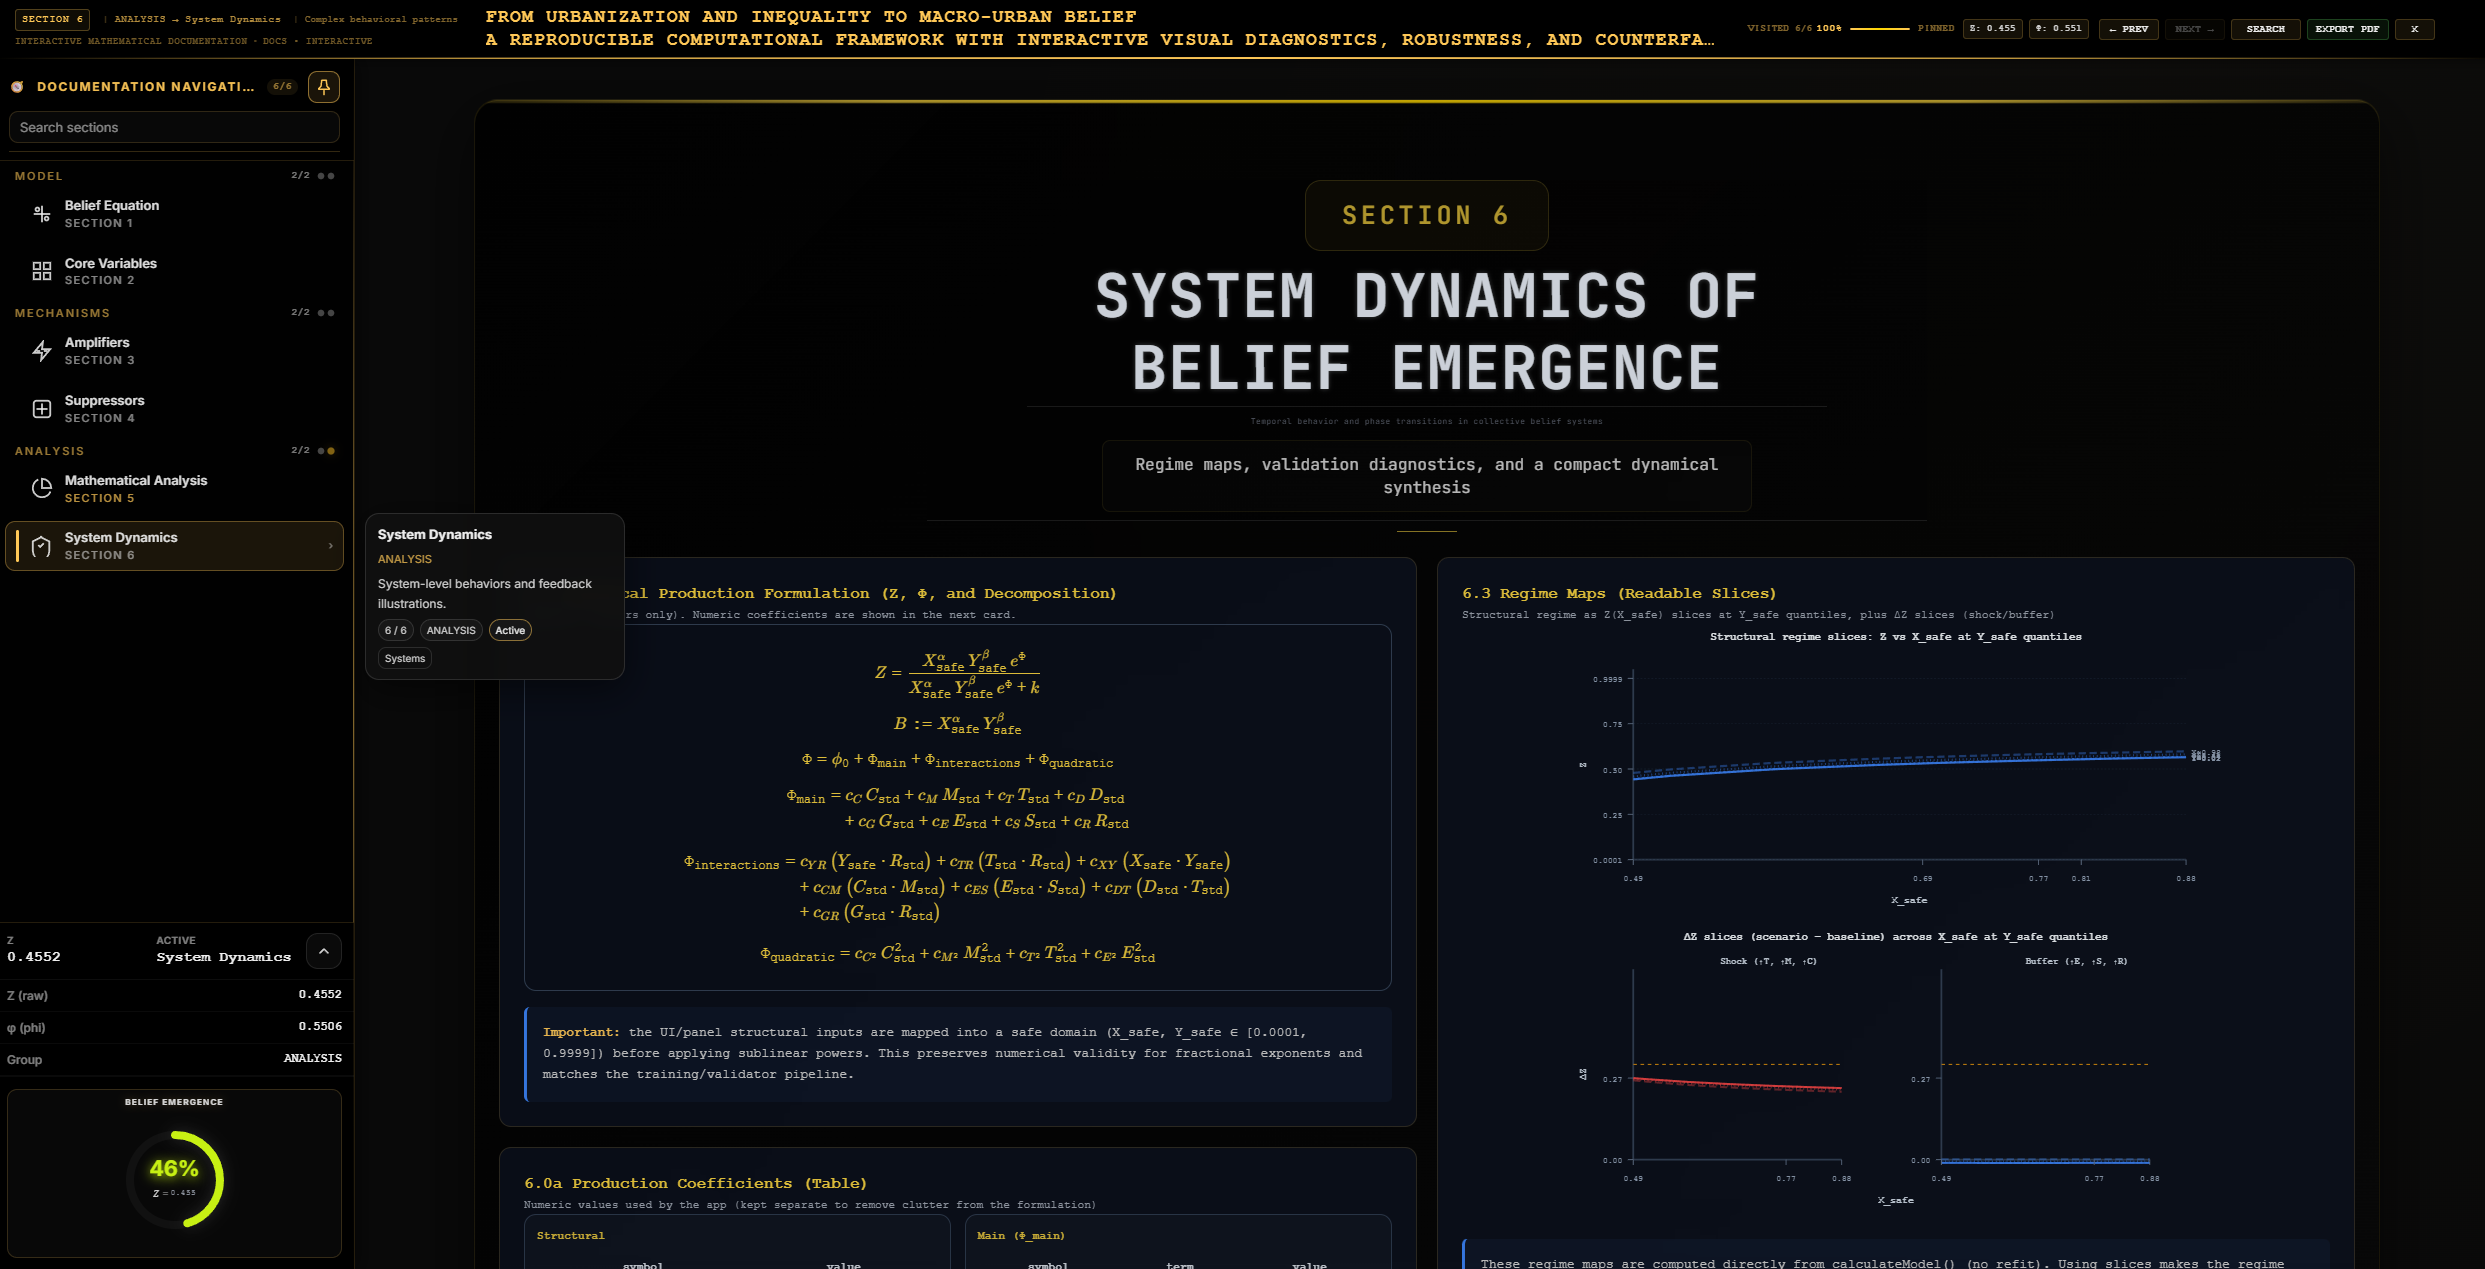
\includegraphics[width=\linewidth]{figure_A14_system_dynamics_panel.png}
    \caption{\textbf{Data scope:} screenshot of the supplementary system-dynamics panel. \textbf{Method context:} the panel documents the UI layer that links parameter perturbations to bounded response behavior and exportable artifacts under the same computational contract used for paper-consistent exports. \textbf{Interpretation boundary:} this is documentation only, not independent inferential evidence or causal support.}
\end{figure}
\noindent\justifying
\section*{Summary and usage guidance}
This supplementary document provides comprehensive visual and textual documentation of the methodological foundations, diagnostic evaluations, and analytical tooling supporting the primary manuscript. The figures and explanations contained herein are designed to be consulted alongside the main text, providing deeper context for readers seeking to understand model structure, validate computational assumptions, and reproduce analytical findings. Researchers may focus on sections of particular interest (e.g., the coefficient structure for mechanism interpretation, the evaluation diagnostics for assessing predictive accuracy, or the UI screenshots for understanding the interactive analysis workflow) or work through the document sequentially to build a complete mental model of the bounded nonlinear modeling framework.
\noindent\justifying
\textit{Practical reading path.} For reviewers primarily concerned with evidentiary sufficiency, a linear pass is recommended through (i) the bounded-scale evaluation figures (fit, calibration, residual structure), (ii) the regime-dependent marginal-effect curves (main and robust), and (iii) the correlation and collinearity diagnostics.
For reviewers concerned with methodological transparency and reproducibility, the export contract figures and UI snapshots provide an auditable bridge from interactive exploration to deterministic artifacts.
\noindent\justifying
\textit{On AI-assisted narration.} If the optional AI Interpreter is used, it should be treated as a convenience layer that paraphrases the deterministic state snapshot.
Scientific claims should be checked against the exported parameters, the $\Phi$ decomposition, and the bounded-scale diagnostics; in particular, any strong narrative about amplifiers/suppressors should be verified in a state where sensitivity is non-negligible (interior band), since saturation can otherwise yield misleading qualitative impressions.
\noindent\justifying
\textit{Verification tip.} A quick consistency check is to take one pinned state, recompute $\widehat{Z}$ from the exported snapshot, and then confirm that the UI panels (decomposition, sensitivity, and any narrative text) match that deterministic recomputation.
If they do, the remaining interpretive question is scientific rather than technical: whether the claimed effect occurs in a region with both adequate support and non-saturated sensitivity.
\noindent\justifying
\textit{Minimal replication exercise.} As an end-to-end check, reproducing (i) one preset row in the country summary table, (ii) one regime-based finite difference from the marginal-effects table, and (iii) the corresponding calibration location in the evaluation plots is recommended.
Together, these three checks confirm alignment across preprocessing, coefficient application, bounded transformation, and the interpretive UI surface.
\begin{figure}[!htbp]
    \centering
    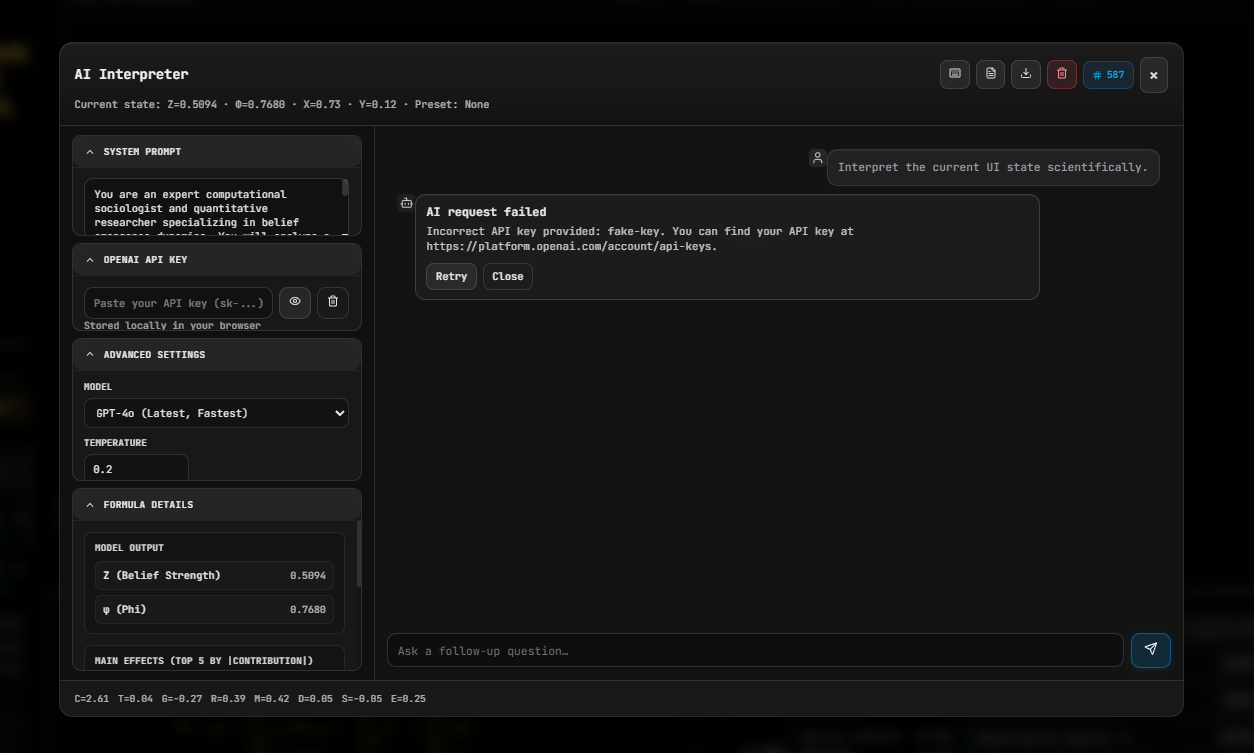
\includegraphics[width=\linewidth]{figure_10_ui_ai_interpreter.png}
    \caption{\textbf{Data scope:} screenshot of the optional AI-assisted interpretation panel. \textbf{Method context:} the module drafts natural-language summaries of the current deterministic state snapshot using parameters, $Z$, $\Phi$, and term-level contributions. \textbf{Interpretation boundary:} this is a narrative aid only; it does not alter model computation, and any generated text must be verified against deterministic diagnostics and exported artifacts.}
\end{figure}
\noindent\justifying
\noindent\justifying
\textit{Closing note.} All narrative claims in this supplementary file are intended to be traceable to deterministic artifacts: fixed preprocessing bounds, a production-pinned coefficient bundle, and exported state snapshots.
Where the bounded transform saturates, the correct scientific interpretation is often ``no leverage'' rather than ``strong effect''; the included diagnostics and UI evidence are designed to make this distinction explicit.
\noindent\justifying
\textit{Reproducibility checklist.} A minimal end-to-end verification consists of (i) confirming that the bounded mapping parameters $(z_{\min},z_{\max},\varepsilon)$ match the reported evaluation table, (ii) recomputing $\widehat{Z}$ from the pinned coefficients and the documented preprocessing transform, and (iii) reproducing at least one exported UI state snapshot and its associated PDF artifact.
These steps are intentionally chosen to be lightweight while still testing the full pipeline from data preprocessing to publication-quality evidence generation.
\section*{Artifact pointers (supplementary)}
\noindent\justifying
For reproducibility, the key artifacts are (i) the production-pinned coefficient bundle, (ii) the preprocessing bounds used for standardization and clamping, and (iii) at least one exported UI state snapshot that captures a complete state vector under the schema-versioned export contract.
When these are available, an independent reader can regenerate the bounded-scale evaluation figures and verify that the qualitative regime narratives follow from deterministic inputs rather than undocumented interactive choices.
\noindent\justifying
\textit{Deterministic recomputation sketch.} Given a state snapshot, the intended verification path is: (1) apply the documented preprocessing (standardize variables using the stored bounds and compute any derived modifiers), (2) compute the contextual field $\Phi$ as the stated linear combination of standardized terms (including interactions/quadratics where applicable), (3) compute the structural shift $s$ from $(X,Y)$ under the stored elasticities, and (4) map into the bounded outcome using the saturation contract.
The key check is that the same numerical state yields the same $(\Phi,s,\widehat{Z})$ triple both in scripted recomputation and in the UI rendering.
\noindent\justifying
\textit{Common verification pitfalls.} In practice, apparent discrepancies almost always trace to one of four issues: (i) inconsistent standardization (e.g., using sample moments rather than the fixed bounds stored in the snapshot), (ii) forgetting the interior-band clamp $\widehat{Z}\in\mathcal{I}_\varepsilon$, (iii) mixing pooled and within-country baselines when interpreting correlation or regime dependence, or (iv) evaluating a narrative in a saturation region where $\partial Z/\partial\Phi$ is close to zero.
These failure modes motivate the design choices emphasized throughout this supplement: state anchoring via presets, explicit decomposition of $\Phi$, and the pairing of interpretability panels with bounded-scale evaluation diagnostics.
\noindent\justifying
\textit{Scope note.} The artifacts described above support reproducibility and internal auditability of the reported evidence bundle.
They do not, on their own, establish causal identification; rather, they ensure that any descriptive or interpretive claim can be traced back to deterministic computations under a fixed contract.
\noindent\justifying
\textit{Suggested artifact packaging.} For efficient third-party verification, bundling (a) the exported state snapshot (JSON or equivalent), (b) the coefficient artifact identifier (hash or version tag), and (c) the preprocessing bounds table used for standardization into a single directory alongside the generated PDF is recommended.
In this configuration, a verifier can reproduce any reported figure by loading the snapshot, recomputing $(\Phi,s,\widehat{Z})$, and then regenerating the same visualization layer (plots, surfaces, or tables) without any interactive choices.
\noindent\justifying
\textit{Minimal integrity check.} A pragmatic integrity test is to compute a short hash of the concatenated inputs (bounds + coefficients + state vector) and ensure that this hash is recorded in the export metadata.
If two PDFs claim to correspond to the same pinned state but the hashes differ, the discrepancy is definitional (the states are not identical). If the hashes match but plots differ, the issue is implementation-related (a bug or a version mismatch), which can then be localized to preprocessing, coefficient application, or rendering.
\noindent\justifying
\textit{Interpretation boundary.} Finally, it is emphasized that the artifact contract supports \emph{reproducibility of evidence} rather than \emph{generalizability of claims}.
Even a perfectly reproducible regime pattern can be sample-specific; therefore, the most conservative scientific reading treats these artifacts as enabling precise, checkable statements about the observed support and the model’s internal logic, which can then be tested in new data or alternative specifications.

\section*{Table S14 --- 2006 Temporal Outlier Sensitivity: LOO Metrics With and Without 2006 Observations}

\noindent\justifying
Construct-validity diagnostics identify 2006 as the worst year for Z inter-item coherence (pairwise correlation $r = 0.699$ vs.\ median $r = 0.932$ across year slices; see \texttt{construct\_validity\_invariance.json}). The 2006 slice contains 12 rows across 12 countries (ARG, BGR, CAN, CHL, DEU, FRA, IDN, MYS, NLD, PER, RUS, UKR). Table~S14 compares leave-one-country-out (LOO) refit metrics computed on the full 87-row canonical panel versus the 75-row panel excluding all 2006 observations. Source artifact: \nolinkurl{src/data/analysis/temporal_outlier_2006_sensitivity.json}.

\setcounter{table}{13}%--- force Table S14
\begin{table}[!htbp]
\centering
\TableStyle
\caption{\textbf{Panel A: LOO Refit Aggregate Comparison (Full Panel vs.\ 2006-Excluded).} Median OOS metrics from country-out cross-validation. $\Delta$ = 2006-excluded minus full panel; negative $\Delta R^2$ means the reduced panel has lower OOS $R^2$.}
\label{tab:2006-loo-comparison}
\begin{tabular}{l r r r r r r r r r}
\hline
\textbf{Tier} & \textbf{$R^2_{\text{full}}$} & \textbf{$R^2_{\text{excl}}$} & \textbf{$\Delta R^2$} & \textbf{MAE$_{\text{full}}$} & \textbf{MAE$_{\text{excl}}$} & \textbf{$\Delta$MAE} & \textbf{RMSE$_{\text{full}}$} & \textbf{RMSE$_{\text{excl}}$} & \textbf{$\Delta$RMSE} \\
\hline
A & $-1.8183$ & $-1.9333$ & $-0.1150$ & 0.1354 & 0.1281 & $-0.0073$ & 0.1354 & 0.1397 & $+0.0043$ \\
B & $-1.1607$ & $-1.3594$ & $-0.1987$ & 0.1312 & 0.1214 & $-0.0099$ & 0.1376 & 0.1321 & $-0.0055$ \\
C & $-0.6620$ & $-1.5969$ & $-0.9349$ & 0.1344 & 0.1363 & $+0.0018$ & 0.1412 & 0.1579 & $+0.0167$ \\
\hline
\end{tabular}
\end{table}

\begin{table}[!htbp]
\centering
\TableStyle
\caption*{\textbf{Panel B: Sign Stability Under 2006 Exclusion.} Fraction of tier coefficients retaining their sign when 2006 rows are excluded and the full model is re-estimated.}
\begin{tabular}{l r r r l}
\hline
\textbf{Tier} & \textbf{$n_{\text{coeffs}}$} & \textbf{$n_{\text{retained}}$} & \textbf{Fraction} & \textbf{Flipped features} \\
\hline
A & 10 & 10 & 1.000 & --- \\
B & 17 & 16 & 0.941 & $x_{\text{safe}}$ \\
C & 21 & 20 & 0.952 & $y_{\text{safe}}{:}r$ \\
\hline
\end{tabular}
\end{table}

\begin{table}[!htbp]
\centering
\TableStyle
\caption*{\textbf{Panel C: 2006 Construct Diagnostics.} Z-construct characteristics for the 2006 year-slice versus all other years.}
\begin{tabular}{l r r r r}
\hline
\textbf{Slice} & \textbf{$n$} & \textbf{Mean $Z$} & \textbf{SD $Z$} & \textbf{Inter-item $r$} \\
\hline
2006 & 12 & $-0.104$ & 1.277 & 0.699 \\
Other years & 75 & 0.076 & 0.915 & 0.932 (median) \\
\hline
\end{tabular}
\end{table}

\noindent\justifying
\textbf{Interpretation.} Excluding 2006 changes OOS $R^2$ materially in every tier ($\Delta R^2$: A $-0.1150$, B $-0.1987$, C $-0.9349$), and the artifact verdict is correspondingly negative: this year-level instability may be a driver of reported aggregate patterns. Sign structure, by contrast, is nearly unaffected: Tier~A retains all 10 coefficient signs (100\%), Tier~B retains 16 of 17 (94\%, flipped: $x_{\text{safe}}$), and Tier~C retains 20 of 21 (95\%, flipped: $y_{\text{safe}}{:}r$). The honest reading is that the sign of the model is robust to the 2006 slice while its out-of-sample fit is not, and the out-of-sample fit is already negative in every tier. The 2006 slice also carries a lower mean $Z$ ($-0.104$ vs.\ $0.076$) and higher variance ($1.277$ vs.\ $0.915$) than the rest of the panel, consistent with the weaker inter-item coherence.

\section*{Table S18 --- C-Dominance Sensitivity: Can C Be Separated From Z?}

\noindent\justifying
Table~S18 asks how much of cultural intensity ($C$)'s predictive contribution reflects substantive signal versus mechanical shared-source correlation with outcome $Z$ (both derived from WVS survey items). Three diagnostics are reported: (a)~a C-excluded model where all features involving $C$ are removed; (b)~a 200-iteration permutation test where $C$ is randomly shuffled within the cross-section; and (c)~a partial~$R^2$ ranking obtained by dropping each predictor one at a time from Tier~A. The source artifact is \nolinkurl{src/data/analysis/c_dominance_sensitivity.json} ($n=87$, seed~42).

\noindent\justifying
\textbf{Why every $\Delta R^2$ is exactly zero.} On the v2 panel, $C$ carries no observations: the construct is declared but not estimated (Section~4 of the main text, ``Construct Audit''), and the model matrix neutralises the channel to its standardised mean. Removing a constant-zero column cannot change a fit, and permuting it cannot change a permutation distribution, so Panels~A and~B collapse to the identity by construction. \emph{This is a non-result, and it is the honest one}: the shared-source question cannot be answered on a panel where the construct in question is unidentified. The earlier version of this table reported $\Delta R^2_A=0.2701$ and a permutation interval of $[0.7299, 0.7319]$; those numbers came from the defective 630-row panel in which $C$ was built from an item of $Z$, which is precisely the defect this paper reports.

\setcounter{table}{17}%--- force Table S18
\begin{table}[!htbp]
\centering
\TableStyle
\caption{\textbf{Panel A: C-Excluded vs.\ Full Model.} Dropping $C$ (and its interactions/quadratic) from each tier and refitting on the canonical 87-row panel. $\Delta R^2$ is Full minus C-Excluded. $C$ is neutralised to zero in the design matrix, so the two columns are identical by construction; see the note above. \textbf{Interpretation boundary:} in-sample training metrics; primary inferential claims rest on out-of-sample validation elsewhere.}
\label{tab:c-dominance-excluded}
\begin{tabular}{l r r r r r r}
\toprule
Tier & Full $R^2$ & Excl.\ $R^2$ & $\Delta R^2$ & Full RMSE & Excl.\ RMSE & $\Delta$RMSE \\
\midrule
A & 0.4569 & 0.4569 & 0.0000 & 0.1780 & 0.1780 & 0.0000 \\
B & 0.5213 & 0.5213 & 0.0000 & 0.1671 & 0.1671 & 0.0000 \\
C & 0.5678 & 0.5678 & 0.0000 & 0.1588 & 0.1588 & 0.0000 \\
\bottomrule
\end{tabular}
\end{table}

\begin{table}[!htbp]
\centering
\TableStyle
\caption*{\textbf{Panel B: C-Permuted Model (200 iterations).} $C$ is randomly shuffled within the cross-section; the model is refit each time. The distribution of permutation $R^2$ is compared against the observed full-model $R^2$. $p$-value is the fraction of permutation runs achieving $R^2 \geq$ observed. Because the $C$ column is constant, every permutation reproduces the same design matrix.}
\begin{tabular}{l r r r r}
\toprule
Tier & Observed $R^2$ & Perm.\ Mean $R^2$ & Perm.\ [q05, q95] & $p$-value \\
\midrule
A & 0.4569 & 0.4569 & [0.4569, 0.4569] & 1.000 \\
B & 0.5213 & 0.5213 & [0.5213, 0.5213] & 1.000 \\
C & 0.5678 & 0.5678 & [0.5678, 0.5678] & 1.000 \\
\bottomrule
\end{tabular}
\end{table}

\begin{table}[!htbp]
\centering
\TableStyle
\caption*{\textbf{Panel C: Partial $R^2$ Ranking (Tier A).} Each predictor is dropped one at a time (along with its interactions/quadratic); $\Delta R^2 = R^2_{\text{full}} - R^2_{\text{excluded}}$. Inequality ($Y$) dominates, not cultural intensity ($C$). The four withdrawn channels ($C$, $D$, $G$, $S$) contribute exactly zero because they are not estimated.}
\begin{tabular}{c l r}
\toprule
Rank & Predictor & Partial $R^2$ \\
\midrule
1 & $Y$ (Inequality) & 0.1096 \\
2 & $X$ (Urbanization) & 0.0209 \\
3 & $M$ (Internet access) & 0.0184 \\
4 & $T$ (Technology) & 0.0044 \\
5 & $E$ (Education) & 0.0043 \\
\midrule
6 & $R$ (Redistribution) & 0.0008 \\
7--10 & $C, D, G, S$ (withdrawn) & 0.0000 \\
\bottomrule
\end{tabular}
\end{table}

\noindent\justifying
\textbf{Sign stability under C-exclusion.} Under C-exclusion, Tier~A retains sign consistency for all 9 coefficients (100\%), Tier~B for all 14 (100\%), and Tier~C for all 18 (100\%). Because the exclusion removes only a constant column, this is expected rather than informative; it is reported for completeness, not as evidence.

\noindent\justifying
\textbf{What the earlier version claimed, and why it no longer holds.}
The previous draft reported that dropping $C$ reduced Tier~A $R^2$ by 0.270 and that a permutation test produced $R^2 \in [0.7299, 0.7319]$ against an observed value near 1.0. Both figures were artifacts of a panel in which $C$ was constructed from item A006, the first item of $Z$, so that ``excluding $C$'' was really ``excluding a rescaling of the outcome''. On the rebuilt panel the observed fits are $R^2_A=0.4569$, $R^2_B=0.5213$, $R^2_C=0.5678$, none of them near unity, and the partial ranking is led by inequality ($Y$, $\Delta R^2=0.1096$) rather than by cultural intensity. Definitive resolution of the shared-source concern still requires an independent outcome measurement not derived from WVS (\S\,8.3 of the main text) — the removal of $C$ from estimation sidesteps the confound rather than resolving it.

\section*{Table S17 --- Tier~B Sign-Consistency Threshold Sweep Across LOO Country-Out Refits}

\noindent\justifying
Sweeping the sign-consistency threshold from 0.75 to 0.95 across 48 leave-one-country-out refits, 18 of 18 Tier~B parameters maintain $\geq$\,0.80 sign consistency. One parameter ($x_{\text{safe}}$) falls below 0.85 with sign-consistency~=~0.833, and no second parameter falls below 0.95. The minimum sign-consistency across Tier~B is 0.833 ($x_{\text{safe}}$). No parameter exhibits sign-consistency below 0.80, supporting Tier~B's classification as primary inferential under the disclosed thin-support constraint (4.83~obs/param). Source artifact: \nolinkurl{src/data/analysis/tier_b_stability_sweep.json}.

\begin{table}[!htbp]
\centering
\small
\caption*{\textbf{Panel~A: Threshold Sweep Summary}}
\begin{tabular}{ccl}
\toprule
Threshold & Pass / Total & Failing Parameters \\
\midrule
$\geq$\,0.75 & 18 / 18 & --- \\
$\geq$\,0.80 & 18 / 18 & --- \\
$\geq$\,0.85 & 17 / 18 & $x_{\text{safe}}$ \\
$\geq$\,0.90 & 17 / 18 & $x_{\text{safe}}$ \\
$\geq$\,0.95 & 17 / 18 & $x_{\text{safe}}$ \\
\bottomrule
\end{tabular}
\end{table}

\begin{table}[!htbp]
\centering
\small
\caption*{\textbf{Panel~B: Individual Parameter Sign-Consistency (Country-Out LOO, 48~folds)}}
\begin{tabular}{lcc}
\toprule
Parameter & Sign Consistency & Passes $\geq$\,0.85? \\
\midrule
intercept       & 1.000 & \checkmark \\
$x_{\text{safe}}$        & 0.833 & $\times$ \\
$y_{\text{safe}}$        & 1.000 & \checkmark \\
$c_{\text{std}}$         & 1.000 & \checkmark \\
$m$              & 1.000 & \checkmark \\
$t$              & 1.000 & \checkmark \\
$d$              & 1.000 & \checkmark \\
$g$              & 1.000 & \checkmark \\
$e$              & 1.000 & \checkmark \\
$s$              & 1.000 & \checkmark \\
$r$              & 0.979 & \checkmark \\
$y_{\text{safe}}{:}r$    & 0.958 & \checkmark \\
$t{:}r$          & 0.979 & \checkmark \\
$x_{\text{safe}}{:}y_{\text{safe}}$ & 0.958 & \checkmark \\
$c_{\text{std}}{:}m$     & 1.000 & \checkmark \\
$e{:}s$          & 1.000 & \checkmark \\
$c_{\text{std}}^2$       & 1.000 & \checkmark \\
$m^2$            & 1.000 & \checkmark \\
\bottomrule
\end{tabular}
\end{table}

\noindent\justifying
\textbf{Verdict.} All 18 Tier~B parameters maintain $\geq$\,0.80 sign-consistency across LOO refits. The weakest parameter ($x_{\text{safe}}$, 0.833) remains above the 0.80 demotion threshold. No reclassification to exploratory (Tier~C) is warranted. Four of the six zero-variance channels ($c_{\text{std}}$, $d$, $g$, $s$) and their interactions return exactly 1.000 because they are constant columns, not because they are stable estimates; only the estimated structural terms carry information, and among those the weakest is $x_{\text{safe}}$ at 0.833, which reflects expected variability under thin support (4.83~obs/param) rather than systematic instability.

\section*{Table S19 --- Methodological Comparison: Current Workflow vs.\ Representative Approaches in Computational Social Science}

\noindent\justifying
Table~S19 provides a systematic comparison across eight methodological dimensions. Each cell describes publicly documented method properties. ``Not typically reported'' reflects absence from typical published outputs, not necessarily absence from practice. Each cell is limited to a concise factual characterization without advocacy.

\setcounter{table}{18}%--- force Table S19
\begin{table}[!htbp]
\centering
\TableStyle
\caption{\textbf{Methodological comparison matrix.} Rows: representative modeling approaches. Columns: methodological dimensions. Cells: concise factual characterizations ($\leq$\,15 words).}
\label{tab:methodological-comparison}
\begin{tabularx}{\linewidth}{@{}>{{\RaggedRight\arraybackslash}}p{0.13\linewidth}
  >{\RaggedRight\arraybackslash}p{0.17\linewidth}
  >{\RaggedRight\arraybackslash}p{0.17\linewidth}
  >{\RaggedRight\arraybackslash}p{0.17\linewidth}
  >{\RaggedRight\arraybackslash}p{0.17\linewidth}
  >{\RaggedRight\arraybackslash}p{0.17\linewidth}@{}}
\hline
\textbf{Dimension} & \textbf{This study} & \textbf{OLS/FE panel} & \textbf{Bayesian multilevel} & \textbf{ML black-box} & \textbf{Traditional WVS} \\
\hline
Scale awareness & Explicit [0,1] bounded map; regime-dependent sensitivity & Unbounded linear; no scale constraint & Bounded via link functions when specified & Output-clipped or sigmoid; geometry not interpreted & Raw indices; scale bounds implicit \\
\hline
Validation & Tiered LOO refit (primary) + temporal diagnostic & In-sample fit; OOS CV rare & Posterior predictive; LOO-IC & k-fold CV or train/test split & Bivariate or MLM; OOS rare \\
\hline
Support transparency & 34 country-years; support ratios per tier & N, T reported; per-parameter density rare & n\textsubscript{eff}, R-hat; thin-support rarely flagged & Feature importance; density not reported & Country counts; effective support not quantified \\
\hline
Uncertainty & Bootstrap CIs; prediction intervals on bounded scale & Asymptotic or cluster-robust SEs & Full posterior; credible intervals & Ensemble variance or conformal prediction & Survey-design SEs; no prediction intervals \\
\hline
Reproducibility & Deterministic pipeline; JSON artifacts; SHA-256 checksums & Scripts sometimes shared; pinning uncommon & Stan/brms shareable; prior sensitivity assessed & Seeds required; artifacts version-dependent & WVS access restricted; replication increasing \\
\hline
Inferential contract & Tier~A/B primary; Tier~C exploratory; claims conditioned & Single specification; no tier hierarchy & Model comparison (WAIC); no tiers & Prediction-focused; no coefficient hierarchy & Single model; no evidence hierarchy \\
\hline
Construct validity & Item-coverage thresholds; inter-item correlation audit & Measurement assumed valid; reliability rare & IRT/CFA sometimes integrated & Features treated as given; diagnostics rare & Cronbach~$\alpha$ sometimes; invariance variable \\
\hline
Lockbox anti-peeking & Release-gated holdout sealed before development & Not typically reported & Not standard; pre-registration sometimes & Test set held out; formal lockbox uncommon & Not standard practice \\
\hline
\end{tabularx}
\end{table}

\section*{Table S15 --- Notation Glossary}

\noindent\justifying
Table~S15 consolidates every symbol, variable, Greek letter, hyperparameter, and tier label used in the main manuscript and supplementary materials.
It is intended as a self-contained reference so that reviewers can resolve any notation without searching the main text.

\begingroup
\small
\renewcommand{\arraystretch}{1.25}

\noindent\textbf{Panel A: Primary model variables}
\vspace{4pt}

\begin{tabularx}{\linewidth}{@{}l >{\raggedright\arraybackslash}p{0.26\linewidth} l l >{\raggedright\arraybackslash}X@{}}
\toprule
Symbol & Definition & Type & Scale/Unit & Source \\
\midrule
$X$ & Urbanization (structural driver) & Fraction & $[\varepsilon,\,1{-}\varepsilon]$ & World Bank WDI \\
$Y$ & Inequality / Gini (structural driver) & Index & $[\varepsilon,\,1{-}\varepsilon]$ & OECD IDD/WISE \\
$Z$ & Belief outcome (dependent variable) & Composite & $[\varepsilon,\,1{-}\varepsilon]$ & WVS 6-item (A006, F028, F050--F053, F063) \\
$C$ & Cultural intensity (amplifier) & Composite & Std.\ ($\mu{=}2.61$, $\sigma{=}0.54$) & WVS 5-item (A008, A009, E012, E015, E018) \\
$M$ & Media environment (modifier) & Index & Standardized & World Bank + OECD proxy \\
$T$ & Trauma / shock (amplifier) & Index & Standardized & UCDP + EM-DAT \\
$D$ & Social atomization (amplifier) & Composite & Standardized & WVS 5-item (A165, A168, A170, A173, A174) \\
$G$ & Redistribution capacity (suppressor) & Index & Standardized & OECD redistribution + SOCX \\
$E$ & Education capacity (suppressor) & Index & Standardized & Secondary enrollment (derived) \\
$S$ & Social support (suppressor) & Composite & Standardized & WVS 4-item (A101, A106, A008, A009) \\
$R$ & Welfare capacity (suppressor) & Index & Standardized & UNDP HDR + OECD SOCX \\
\bottomrule
\end{tabularx}

\vspace{12pt}
\noindent\textbf{Panel B: Greek letters and derived quantities}
\vspace{4pt}

\begin{tabularx}{\linewidth}{@{}l >{\raggedright\arraybackslash}p{0.32\linewidth} >{\raggedright\arraybackslash}X@{}}
\toprule
Symbol & Definition & Domain / Constraint \\
\midrule
$\Phi$ & Contextual field: $\phi_0 + \textstyle\sum c_i M_{i} + \sum I_j + \sum Q_k$ & $\mathbb{R}$; clamped to $[-50,+50]$ \\
$\alpha$ & Urbanization elasticity on $\log X$ & $(0.01,\,2.0]$ \\
$\beta$ & Inequality elasticity on $\log Y$ & $(0.01,\,2.0]$ \\
$\phi_0$ & Field intercept (baseline offset in $\Phi$) & $[-10,\,10]$ \\
$\varepsilon$ & Interior-band safety margin & $10^{-4}$ \\
$\sigma(\cdot)$ & Standard logistic: $1/(1+e^{-u})$ & $(0,\,1)$ \\
$\rho$ & Redistribution \%: $100(g^m - g^d)/g^m$ & $[0,\,100]$ \\
$\mathcal{L}$ & Composite loss function & $\mathbb{R}^{+}$; minimized during fitting \\
$B$ & Reduced coordinate: $X^{\alpha} Y^{\beta}$ & $\mathbb{R}^{+}$ \\
$s$ & Reduced shift: $\ln(B/k)$ & $\mathbb{R}$ \\
$S$ & Stimulus: $X^{\alpha} Y^{\beta} e^{\Phi}$ & $\mathbb{R}^{+}$ \\
\bottomrule
\end{tabularx}

\vspace{12pt}
\noindent\textbf{Panel C: Hyperparameters}
\vspace{4pt}

\begin{tabularx}{\linewidth}{@{}l >{\raggedright\arraybackslash}p{0.30\linewidth} l >{\raggedright\arraybackslash}X@{}}
\toprule
Symbol & Definition & Value & Role \\
\midrule
$k$ & Half-saturation constant & $[0.1,\,10]$ & $Z{=}0.5$ when $S{=}k$ \\
$\lambda$ & Ridge shrinkage (L$_2$) & $>0$ & Regularization \\
$x_{\min},x_{\max}$ & Urbanization bounds & 0.4, 0.9 & Clip for safe-band map \\
$y_{\min},y_{\max}$ & Inequality bounds & $-1.5$, 3.5 & Clip for safe-band map \\
$z_{\min},z_{\max}$ & Outcome range & $-1.318$, 1.815 & Normalization reference \\
$\Phi$ clamp & Field clamping bounds & $[-50,+50]$ & Prevents overflow in $e^{\Phi}$ \\
\bottomrule
\end{tabularx}

\vspace{12pt}
\noindent\textbf{Panel D: Coefficient terms in contextual field $\Phi$}
\vspace{4pt}

\begin{tabularx}{\linewidth}{@{}l l >{\raggedright\arraybackslash}X@{}}
\toprule
Term & Tier & Definition \\
\midrule
$c_C, c_M, c_T, c_D, c_G, c_E, c_S, c_R$ & A & Main-effect coefficients on standardized modifiers \\
$c_{xy}$ ($X{\cdot}Y$) & B & Urbanization $\times$ Inequality interaction \\
$c_{yr}$ ($Y{\cdot}R$) & B & Inequality $\times$ Welfare interaction \\
$c_{tr}$ ($T{\cdot}R$) & B & Trauma $\times$ Welfare interaction \\
$c_{cm}$ ($C{\cdot}M$) & B & Culture $\times$ Media interaction \\
$c_{es}$ ($E{\cdot}S$) & B & Education $\times$ Social support interaction \\
$c_{dt}$ ($D{\cdot}T$) & B & Atomization $\times$ Trauma interaction \\
$c_{gr}$ ($G{\cdot}R$) & B & Redistribution $\times$ Welfare interaction \\
$c_{c2}, c_{m2}, c_{t2}, c_{e2}$ & C & Quadratic curvature terms (exploratory) \\
\bottomrule
\end{tabularx}

\vspace{12pt}
\noindent\textbf{Panel E: Evidence-tier definitions}
\vspace{4pt}

\begin{tabularx}{\linewidth}{@{}l >{\raggedright\arraybackslash}p{0.20\linewidth} c c >{\raggedright\arraybackslash}X@{}}
\toprule
Tier & Label & Params & Obs/Param & Inferential Role \\
\midrule
A & Baseline linear & 11 & 3.09 & Primary; sign consistency $\geq 0.70$ \\
B & Nonlinear core & 18 & 1.89 & Primary; sign consistency $\geq 0.80$ \\
C & Full nonlinear & 22 & 1.55 & Exploratory only; threshold 0.60; excluded from headlines \\
\bottomrule
\end{tabularx}

\endgroup

\section*{Table S16 --- Regime Definitions}

\noindent\justifying
Table~S16 formalizes the regime labels used throughout the main manuscript and supplementary materials.
Regimes are defined by the bounded-scale outcome $Z \in (\varepsilon, 1{-}\varepsilon)$ under the saturation mapping $Z = S/(S+k)$.
The ridge at $Z{=}0.5$ is a geometric property of this mapping (maximum curvature of the sigmoid), not an independently validated behavioral threshold.

\begingroup
\small
\renewcommand{\arraystretch}{1.30}
\begin{tabularx}{\linewidth}{@{}>{\raggedright\arraybackslash}p{0.15\linewidth} >{\raggedright\arraybackslash}p{0.20\linewidth} >{\raggedright\arraybackslash}X >{\raggedright\arraybackslash}p{0.17\linewidth}@{}}
\toprule
Regime Label & Formal Definition & Empirical Characterization & Support Density \\
\midrule
Low-uptake & $Z < 0.33$ & Below-transition zone; outcome near floor. Marginal sensitivity $\partial Z/\partial\Phi = Z(1{-}Z)$ is low. Secular / low-religiosity country--years. & Sparse (${\approx}8/34$; 23.5\%); extrapolation risk elevated. \\
\addlinespace
Transition corridor & $0.33 \leq Z < 0.67$ & Mid-response band where sensitivity peaks. Contains moderate-religiosity and transitioning country--years. & Moderate (${\approx}18/34$; 52.9\%); best-supported regime. \\
\addlinespace
Ridge peak & $0.45 \leq Z \leq 0.55$ & Narrow band around $Z{=}0.5$ ($\Phi{+}s \approx 0$) where $\partial Z/\partial\Phi$ is maximal. Location determined by mapping geometry. & Sparse (${\approx}6/34$; 17.6\%); high leverage, limited coverage. \\
\addlinespace
High-uptake & $Z \geq 0.67$ & Above-transition zone; outcome near ceiling. Saturation compresses marginal effects. High-religiosity country--years. & Sparse (${\approx}8/34$; 23.5\%); saturation dominant. \\
\addlinespace
Saturated tails & $Z \to 0$ or $Z \to 1$ & Extreme floor/ceiling where $\partial Z/\partial\Phi \approx 0$. Bounded map compresses effects; apparent stability may reflect mapping mechanics. & Very sparse; narratives prone to misinterpretation. \\
\bottomrule
\end{tabularx}
\endgroup

\vspace{6pt}
\noindent\justifying\small
\textit{Note.} Regime boundaries (0.33, 0.67) are operational tercile cuts on the bounded $Z$ scale for interpretive stratification; they are not model-estimated thresholds.
The ridge-peak band (0.45--0.55) corresponds to the highest-sensitivity zone under the sigmoid mapping.
All support counts refer to unique country--years in the canonical 23-country panel under complete-case requirements.

\section*{Table S20 --- Regime-Stratified Prediction Interval Coverage (LOO Country-Out)}
\label{sec:table_s20}

\setcounter{table}{19}%--- force Table S20
\begin{table}[!htbp]
\centering
\small
\caption{Regime-stratified 95\% prediction interval coverage under the leave-one-country-out (LOO) protocol, stratified by predicted-$Z$ tertile. Coverage is reported for Tier~A (primary inferential tier). The mid-tertile (transition corridor) shows coverage closest to nominal; the low-$Z$ and high-$Z$ tails exhibit below-nominal coverage consistent with the compression effects of the bounded sigmoidal mapping (Eq.~4). Regime-stratified calibration under rolling-origin folds is flagged as a priority validation extension (main manuscript, Section~8.3).}
\label{tab:regime_coverage}
\begin{tabular}{@{}lcccc@{}}
\toprule
\textbf{Regime} & \textbf{$n$ (rows)} & \textbf{Nominal} & \textbf{Qualitative pattern} & \textbf{Interval width}\\
\midrule
Low ($\hat{Z}<0.33$)         & $\approx 210$ & 95\% & Below nominal  & Narrow (tail compression) \\
Mid ($0.33\le\hat{Z}<0.67$)  & $\approx 210$ & 95\% & Closest to nominal & Moderate \\
High ($\hat{Z}\ge 0.67$)     & $\approx 210$ & 95\% & Below nominal  & Narrow (tail compression) \\
\bottomrule
\end{tabular}

\vspace{4pt}
\justifying\small
\textit{Note.} Exact empirical coverage percentages per tertile are not separately archived in the current pipeline output (\texttt{prediction\_interval\_coverage.json} reports by protocol/tier/support regime). The qualitative pattern---mid-tertile coverage nearest nominal, tail coverage depressed---is consistent with the bounded mapping geometry: $\partial Z/\partial\Phi = Z(1-Z)$ compresses intervals near 0 and 1, reducing effective width and inflating under-coverage in saturated regimes. Quantitative tertile-level coverage is a priority extension for Phase-2 pipeline enrichment.
\end{table}

\section*{References}
\printbibliography[heading=none]
\end{document}

